\documentclass[11pt,a4paper,oneside]{report}
\usepackage{nabiadoc}
\usepackage{tikz}
\usetikzlibrary{positioning,arrows.meta,fit,calc}
\usepackage{caption}
\usepackage{tabularx}
\usepackage{graphicx}
\usepackage{xurl}  % code paths break at any character
\captionsetup[lstlisting]{justification=raggedright, singlelinecheck=false, font=small, labelfont=bf}
\setcounter{secnumdepth}{2}
\setcounter{tocdepth}{1}

% --- code excerpts and locations, generated at build time by extract_snippets.py ------------------------------
\input{snippets.tex}
\newcommand{\snippetsource}[1]{\csname snippet@#1\endcsname}
\newcommand{\snippet}[3]{%
  \lstinputlisting[language=#2, caption={#3\\{\footnotesize\ttfamily\snippetsource{#1}}}]{#1.txt}}
% A code location as a breakable path (the location is a detokenized string).
\newcommand{\codepath}[1]{\begingroup\edef\x{\csname snippet@#1\endcsname}\expandafter\nolinkurl\expandafter{\x}\endgroup}
\newcommand{\coderef}[1]{{\footnotesize\codepath{#1}}}
\newenvironment{codepointers}{%
  \par\smallskip\begingroup\footnotesize\noindent\textcolor{blue!50!black}{\textbf{Code}}\par\nopagebreak
  \begin{list}{}{\setlength{\leftmargin}{1.2em}\setlength{\itemsep}{0pt}\setlength{\parsep}{0pt}\setlength{\topsep}{1pt}}}%
  {\end{list}\endgroup\smallskip}
\newcommand{\codeitem}[2]{\item #2 --- \codepath{#1}}
% A piece of a whole file (packaging chapter): workflow jobs, pyproject tables, scripts.
\newcommand{\filepiece}[3]{\lstinputlisting[language=#2, caption={#3}]{#1.txt}}
\newcommand{\cmd}{\lstinline[language=bash,basicstyle=\ttfamily\small]}
\newenvironment{note}[1]{\par\medskip\noindent\rule{\linewidth}{0.4pt}\par\nopagebreak\noindent
  \textbf{#1}\enspace}{\par\nopagebreak\noindent\rule{\linewidth}{0.4pt}\par\medskip}

\lstdefinelanguage{yaml}{sensitive=true, comment=[l]{\#}, morestring=[b]", morestring=[b]', keywords={true,false,null}}
\lstdefinelanguage{toml}{sensitive=true, comment=[l]{\#}, morestring=[b]", morestring=[b]', keywords={true,false}}
\lstdefinelanguage{PowerShell}{sensitive=false, comment=[l]{\#}, morecomment=[s]{<\#}{\#>}, morestring=[b]",
  morestring=[b]', keywords={param,if,else,elseif,foreach,throw,try,finally,function,return}}
\lstdefinelanguage{cmake}{sensitive=false, comment=[l]{\#}, morestring=[b]",
  keywords={if,else,endif,install,set,find_package,pybind11_add_module,target_link_libraries,set_target_properties}}
\lstset{basicstyle=\ttfamily\scriptsize, captionpos=t, numbers=none, aboveskip=8pt, belowskip=8pt,
        tabsize=4, keepspaces=true, breaklines=true, postbreak=\mbox{\textcolor{gray}{$\hookrightarrow$}\space}}
\renewcommand{\lstlistingname}{Code}

% --- notation ------------------------------------------------------------------------------------------------
\newcommand{\sth}{\mathcal{S}}                % soft thresholding
\newcommand{\Aeq}{A_{\mathrm{eq}}}
\newcommand{\beq}{b_{\mathrm{eq}}}
\newcommand{\Ain}{A_{\mathrm{in}}}
\newcommand{\bin}{b_{\mathrm{in}}}
\newcommand{\pos}[1]{\left[#1\right]_+}
\newcommand{\anc}{\operatorname{anc}}
\newcommand{\one}{\mathbf 1}
% A figure produced by the pipeline (doc/figures, refreshed by build.sh --figures); skipped if absent.
\newcommand{\pipelinefigure}[3]{\IfFileExists{figures/#1}{\begin{figure}[htbp]\centering
  \includegraphics[width=\linewidth]{figures/#1}\caption{#2}\label{#3}\end{figure}}{}}

\title{nabia\\[0.4em]\Large Methodology, implementation and user guide\\[0.3em]
\large A C++ numerical library, its Python bindings, and sentiment-modulated risk budgeting}
\author{nabia documentation}
\date{October 2026}

\begin{document}
\maketitle

\begin{abstract}
nabia is a platform for researching systematic, risk-budgeted portfolios. This document is its single
reference. It starts with a user guide (building, installing and running every part), then describes the
architecture, every numerical method of the C++ library stated mathematically with proofs where a property
is relied on, the full derivations behind the forecasters, the optimizers and the elastic net, the command-line
application, the Python bindings and how they are packaged as wheels for every platform, the Python package,
and the sentiment-modulated risk-budgeting pipeline: LLM news sentiment and market indicators combined per asset
by an elastic net into a score that modulates risk budgets, long-only or long-short. Throughout, each concept
points to the code that implements it, by file and line range, and the key code is shown in excerpts
\emph{extracted from the source when the document is built}: they are the code that runs, and a renamed
function stops the build instead of leaving a stale reference.
\end{abstract}

\tableofcontents

\part{User guide}\label{part:guide}
% Part I: how to build, install and run every part of nabia.

\chapter{Getting started}\label{ch:guide}

\section{What is in the repository}
\begin{center}\small
\begin{tabularx}{\linewidth}{@{}l l X@{}}
\toprule
Folder & Open in & Contents \\
\midrule
\code{cpp/} & CLion (CMake) & the C++ library (\code{include}, \code{src}), Catch2 tests, the command-line
  backtest, and the pybind11 bindings that build the \code{nabia\_python\_bridge} wheel \\
\code{nabia\_python/} & PyCharm & the Python project: the \code{nabia} package (portfolio backtests, analytics,
  market data, and the sentiment risk-budgeting pipeline \code{nabia.sentiment\_rb}), its tests, its single
  \code{pyproject.toml} and its \code{.venv} \\
\code{doc/} & --- & this document (\code{nabia.tex}, chapters, the snippet extractor, \code{build.sh}) and the
  specification of the sentiment pipeline (\code{sentiment\_risk\_budgeting\_spec.md}) \\
\code{dist/} & --- & built wheels (not versioned) \\
\code{.github/workflows/wheels.yml} & --- & wheels for every platform in GitHub Actions \\
\bottomrule
\end{tabularx}
\end{center}
The two projects meet only through the wheel: \code{cpp/} builds \code{nabia\_python\_bridge} into
\code{dist/}, and \code{nabia\_python/} installs it into its \code{.venv}. The order of the steps below follows
from that.

\section{Prerequisites}
\begin{itemize}
  \item \textbf{C++}: CMake 3.25 or newer and a C++20 compiler (Apple clang from Xcode, GCC 12+, MSVC 2022).
        Eigen, iir1, Catch2, nlohmann/json and pybind11 are found on the system or downloaded by CMake.
  \item \textbf{Python}: CPython 3.10--3.14, and \href{https://docs.astral.sh/uv/}{uv} to build wheels for several
        versions. pdflatex (TeX Live, MacTeX) to build this document.
  \item \textbf{Optional}: the GitHub CLI (\code{gh}, logged in) to download published wheels or start CI; an
        Anthropic API key for the pipeline's \code{--live} mode.
\end{itemize}

\section{Step 1: the C++ library}
\begin{lstlisting}[language=bash]
cd cpp
cmake --preset debug                    # configure (once, or after editing a CMakeLists.txt)
cmake --build --preset debug -j         # library, tests, command-line application, C++ examples
ctest --preset debug                    # the Catch2 suite and an end-to-end run of the application
\end{lstlisting}
Presets: \code{debug}, \code{release}, \code{releaseWithDebugInfo}, \code{asan} (address and undefined-behaviour
sanitizers) and \code{python-bridge} (a development build of the bindings, \S\ref{sec:guide-debug}). In CLion,
open \code{cpp/}; it reads \code{CMakePresets.json}: enable the \code{debug} preset and run or debug
\code{nabia\_tests} or \code{nabia\_rb\_backtest}. The command-line backtest (Chapter~\ref{c:sec:cli}):
\begin{lstlisting}[language=bash]
./build/debug/apps/rb_backtest/nabia_rb_backtest --prices apps/rb_backtest/example/prices.csv \
    --config apps/rb_backtest/example/portfolio.json --output /tmp/result.csv
\end{lstlisting}

\section{Step 2: the wheel}
The bindings are packaged as a wheel, one per Python version (Chapter~\ref{ch:packaging} explains wheels):
\begin{lstlisting}[language=bash]
cpp/scripts/build_wheels.sh 3.14        # the Python version of nabia_python/.venv (no argument: 3.10-3.14)
NABIA_WHEEL_BUILD_TYPE=RelWithDebInfo cpp/scripts/build_wheels.sh 3.14   # with debug symbols
cpp\scripts\build_wheels.ps1 -Versions 3.12   # Windows (PowerShell): cibuildwheel, win_amd64
\end{lstlisting}
Each wheel is built in isolation, installed in a clean environment and tested with
\code{nabia\_python/tests/bridge} before it is copied to \code{dist/}. Instead of building, the wheels published
by the CI can be downloaded: \cmd|nabia_python/scripts/fetch_wheels.sh| (the newest successful run, or
\cmd|fetch_wheels.sh release v0.1.0|).

\section{Step 3: the Python project}
\begin{lstlisting}[language=bash]
nabia_python/scripts/setup_env.sh       # creates nabia_python/.venv: the wheel from dist/ + nabia (editable)
cd nabia_python
.venv/bin/python -m pytest              # the bridge tests, the package tests, the pipeline tests
\end{lstlisting}
\code{setup\_env.sh} (\code{setup\_env.ps1} on Windows) reinstalls the wheel every time, so run it again after
rebuilding the C++ code; Python changes are seen at once (editable install). \code{PYTHON=python3.12} chooses the
interpreter of a new \code{.venv}. In PyCharm, open \code{nabia\_python/} and select \code{.venv/bin/python} as the
interpreter. The whole library is then available from Python (Chapter~\ref{c:sec:bridge}):
\begin{lstlisting}[language=Python]
import nabia_python_bridge as nb
from nabia_python_bridge import frames

rb = nb.risk.RiskBudgeting(nb.risk.RiskBudgetingParams(budgets=[0.5, 0.3, 0.2]), nb.risk.Volatility(cov))
weights = rb.optimize()
reg = frames.regress(fund_returns, factor_returns, min_factors=1, max_factors=3, train_fraction=0.7)
\end{lstlisting}

\section{Step 4: the sentiment risk-budgeting pipeline}
From \code{nabia\_python/} (Part~\ref{part:sentiment} describes the method):
\begin{lstlisting}[language=bash]
.venv/bin/python -m nabia.sentiment_rb                    # long-only, offline (synthetic data, mocked LLM), ~20 s
.venv/bin/python -m nabia.sentiment_rb --show             # also open the figures
.venv/bin/python -m nabia.sentiment_rb --config <(echo '{"budgets": {"mode": "long_short"}}')
.venv/bin/python -m nabia.sentiment_rb --ic-sweep 0 0.1 0.2 0.3 0.5    # alpha against news quality
.venv/bin/python -m nabia.sentiment_rb --out output/my_run             # another output folder
.venv/bin/nabia-sentiment --help                          # the same command, installed as a script
\end{lstlisting}
\begin{itemize}
  \item \textbf{Configuration.} Every setting lives in \code{CONFIG} (\coderef{rb_config}): windows, horizon,
        elastic-net grid, refit schedule, normalization, budget bounds, long-only/long-short, LLM models,
        taxonomy, indicators, assets. \code{--config file.json} deep-merges overrides; long-short mode is
        described in \S\ref{sec:rb-longshort}:
\begin{lstlisting}
{"normalize": {"method": "phi"}, "model": {"refit": "ME"}}
{"budgets": {"mode": "long_short", "short_below": 0.35, "long_above": 0.5, "modulate_long_short": false}}
\end{lstlisting}
  \item \textbf{Live LLM}: \cmd|.venv/bin/pip install -e ".[llm]"|, set \code{ANTHROPIC\_API\_KEY}, add
        \code{--live}: the news of the last \code{llm.live\_days} days is scored by Claude (models in
        \code{llm.triage\_model}, \code{scoring\_model}, \code{digest\_model}); the rest stays mocked.
  \item \textbf{Outputs}, in \code{output/sentiment\_rb} by default:
        \begin{itemize}
          \item tables: \code{comparison}, \code{ic}, \code{llm\_ic}, \code{snapshot}, \code{budgets}, \code{signal},
                \code{selection\_frequency}, \code{ic\_in\_out\_of\_sample}, \code{equity}, \code{news} (CSV);
          \item the LLM audit log \code{llm\_audit.jsonl};
          \item figures \code{portfolio.png}, \code{budgets.png}, \code{model.png}; for a sweep,
                \code{sweep.png} and \code{sweep.csv}.
        \end{itemize}
\end{itemize}

\section{Real data}\label{sec:guide-real}
\begin{lstlisting}[language=bash]
.venv/bin/python -m nabia.sentiment_rb --data real --out output/real          # real prices, example news, offline
.venv/bin/python -m nabia.sentiment_rb --data real --news my_news.json         # your own news file
.venv/bin/python -m nabia.sentiment_rb.data.example_news --ic 0.3             # regenerate the example news
.venv/bin/python -m nabia.sentiment_rb --data real --live --batch --config <(echo '{"llm": {"live_days": 0}}')
.venv/bin/python -m nabia.news fetch --no-rss --gkg --since 2024-01-01    # news history -> data/news.json
.venv/bin/python -m nabia.news fetch                                       # today's RSS items (run daily)
.venv/bin/python -m nabia.news score                                     # local Ollama -> data/news_scores.json
.venv/bin/python -m nabia.sentiment_rb --data real --scores data/news_scores.json
\end{lstlisting}
Prices and indicators come from Yahoo Finance and FRED and are cached in \code{data/cache}; news comes from a JSON
file of articles; live scoring caches every response in \code{data/llm\_cache.jsonl}. Chapter~\ref{ch:rb-real}
describes the three parts.

\section{Run configurations and the weights script}\label{sec:guide-weights}
The settings are in three parts (\coderef{rb_config}). \code{CONFIG} holds the methodology every run shares:
the factor tree, assets, features, windows, model, budgets, portfolio and LLM. \code{SYNTHETIC} and \code{REAL}
hold the data settings of each kind of run. A run's JSON file chooses one with \code{data.source} and overrides any
key: \code{configs/synthetic.json} (generated market and news, the oracle skill) and \code{configs/real.json}
(Yahoo and FRED prices, the news and scores files, the LLM provider).
\begin{lstlisting}[language=bash]
.venv/bin/python -m nabia.sentiment_rb --config configs/synthetic.json --out output/syn   # full report and figures
.venv/bin/python -m nabia.sentiment_rb --config configs/real.json --out output/real
.venv/bin/python scripts/sentiment_weights.py configs/real.json                           # weights only
\end{lstlisting}
\code{scripts/sentiment\_weights.py} takes a single argument, the configuration, and computes the signal, the budgets,
the directions and the weights over a lookback window (\code{backtest.lookback\_days}, ending at
\code{backtest.as\_of}, by default the last date). With \code{data.scores\_file} it reads the LLM scores. Without one,
it scores \code{data.news\_file} with \code{llm.provider}: \code{mock} (offline) or \code{ollama} or
\code{anthropic} (live). An \code{as\_of} date also cuts the data there, so the position uses nothing that came later.
It writes the following to \code{backtest.out}:
\begin{itemize}
  \item \code{signal.csv}: the daily $s$;
  \item \code{rebalances.csv}: per rebalance and asset, $s$, the direction, the budget, the weight and the risk
        contribution;
  \item \code{current.csv}: the position to hold from the as-of date;
  \item \code{summary.json}: that position and the window's performance against plain ERC.
\end{itemize}

\section{The staged real-data pipeline}\label{sec:guide-stages}
Five scripts run the real-data pipeline one step at a time, each from the configuration file alone. Each step
writes a file that the later steps read, so it runs once (\coderef{rb_stages}):
\begin{lstlisting}[language=bash]
.venv/bin/python scripts/pipeline/collect_news_1.py configs/real.json      # articles -> data.news_file
.venv/bin/python scripts/pipeline/digest_news_2.py configs/real.json       # LLM daily digests -> data.digests_file
.venv/bin/python scripts/pipeline/score_news_3.py configs/real.json        # LLM article scores -> data.scores_file
.venv/bin/python scripts/pipeline/calibrate_betas_4.py configs/real.json   # elastic-net betas -> data.betas_file
.venv/bin/python scripts/pipeline/backtest_5.py configs/real.json          # portfolio with the stored betas
\end{lstlisting}
\begin{enumerate}
  \item \textbf{Collect} (section \code{collect}): RSS items and GDELT GKG history, deduplicated, appended to the
        news file. Run it again to add new articles.
  \item \textbf{Digest}: the LLM's macro digest of every day (Prompt C), with \code{llm.provider}.
  \item \textbf{Score}: triage and node scores of every article (Prompts A and B). Steps 2 and 3 save their file every
        25 items and cache every response in \code{llm.cache}, so an interrupted run resumes.
  \item \textbf{Calibrate}: the purged walk-forward elastic net of every asset (Chapter~\ref{ch:rb-model}). The betas
        of every refit date are stored with the asset's candidate features and the model settings
        (\coderef{rb_fit_betas}).
  \item \textbf{Backtest}: each refit's stored betas give $S$ and $s$ from the next day to the next refit
        (\coderef{rb_apply_betas}). The budgets, directions, backtest against ERC, report and positions follow. Betas
        whose features are no longer the run's candidates are refused.
\end{enumerate}
Splitting the calibration from the scoring gives exactly the results of the one-shot run, as a test checks.

\section{Debugging the C++ code from Python}\label{sec:guide-debug}
\begin{enumerate}
  \item Build a wheel with debug symbols (\code{NABIA\_WHEEL\_BUILD\_TYPE=RelWithDebInfo}) and run
        \code{setup\_env.sh}; or, without a wheel, \cmd|cmake --preset python-bridge && cmake --build --preset python-bridge|
        in \code{cpp/}, which writes the modules next to the package sources, and run the script with
        \code{PYTHONPATH=<repository>/cpp/bindings}.
  \item Start the script in PyCharm, stopped at a breakpoint before the C++ call.
  \item In CLion: Run $\to$ Attach to Process, the Python process. Breakpoints in \code{cpp/src} are hit.
\end{enumerate}

\section{Wheels for every platform and releases}
\begin{lstlisting}[language=bash]
gh workflow run wheels.yml                          # Linux x86_64/aarch64, macOS arm64/x86_64, Windows AMD64
gh run list --workflow wheels.yml                   # follow it
gh run download <run-id> -n all-wheels -D dist      # every wheel and the sdist
git tag v0.2.0 && git push origin v0.2.0            # a GitHub Release with all of them attached
\end{lstlisting}
Pushes to \code{main} and pull requests that change \code{cpp/} also start the workflow. Chapter~\ref{ch:packaging}
explains every job and how to write new ones.

\section{Building this document}
\begin{lstlisting}[language=bash]
doc/build.sh                 # doc/nabia.pdf: extracts the excerpts from the current code, runs pdflatex 3 times
doc/build.sh --figures       # first reruns the pipeline (long-only, long-short, both sweeps) for the figures/tables
\end{lstlisting}
The excerpts, their file:line locations and the packaging file pieces are extracted from the repository by
\code{doc/extract\_snippets.py}; a function that no longer exists stops the build. The figures and result tables
of Part~\ref{part:sentiment} are copied from \code{nabia\_python/output} into \code{doc/figures} by
\code{--figures}.


\part{Architecture}\label{part:architecture}
% Part II: what nabia is for and how its parts fit together.

\chapter{Purpose and architecture}\label{ch:architecture}

\section{Purpose}
nabia researches \emph{systematic, risk-budgeted portfolios} across equity indices, government bond and credit
markets, and commodities. A strategy has four stages, and the project provides a component for each:
\begin{enumerate}
  \item \textbf{Signals}: filters and forecasters that extract trends from noisy prices (Chapters~\ref{c:sec:signal}
        and~\ref{c:sec:forecast}), a factor regression engine (Chapter~\ref{c:sec:regression}), and news sentiment
        produced by a language model and combined with market indicators per asset (Part~\ref{part:sentiment}).
  \item \textbf{Allocation}: \emph{risk budgeting} decides each asset's share of portfolio risk
        (Chapter~\ref{c:sec:riskbudgeting}); the sentiment pipeline modulates those budgets, or the side of each
        position (long or short).
  \item \textbf{Simulation}: a walk-forward engine turns budgets into weights at each rebalance, without
        look-ahead, and accounts for drift and costs (Chapter~\ref{c:sec:engine}).
  \item \textbf{Evaluation}: performance metrics (Chapter~\ref{c:sec:metrics}), information coefficients and
        in-sample versus out-of-sample diagnostics (Part~\ref{part:sentiment}).
\end{enumerate}
The central design decision is to separate \emph{what decides the risk budgets} (a fixed rule, equal risk, or
the sentiment model) from \emph{how budgets become positions} (a tested numerical engine). A signal never sets
weights directly: it changes budgets within bounds, or the side of a position, and the engine computes the
weights, so each decision is bounded and reproducible from its stored budgets.

\section{Components}
\begin{figure}[ht]
\centering
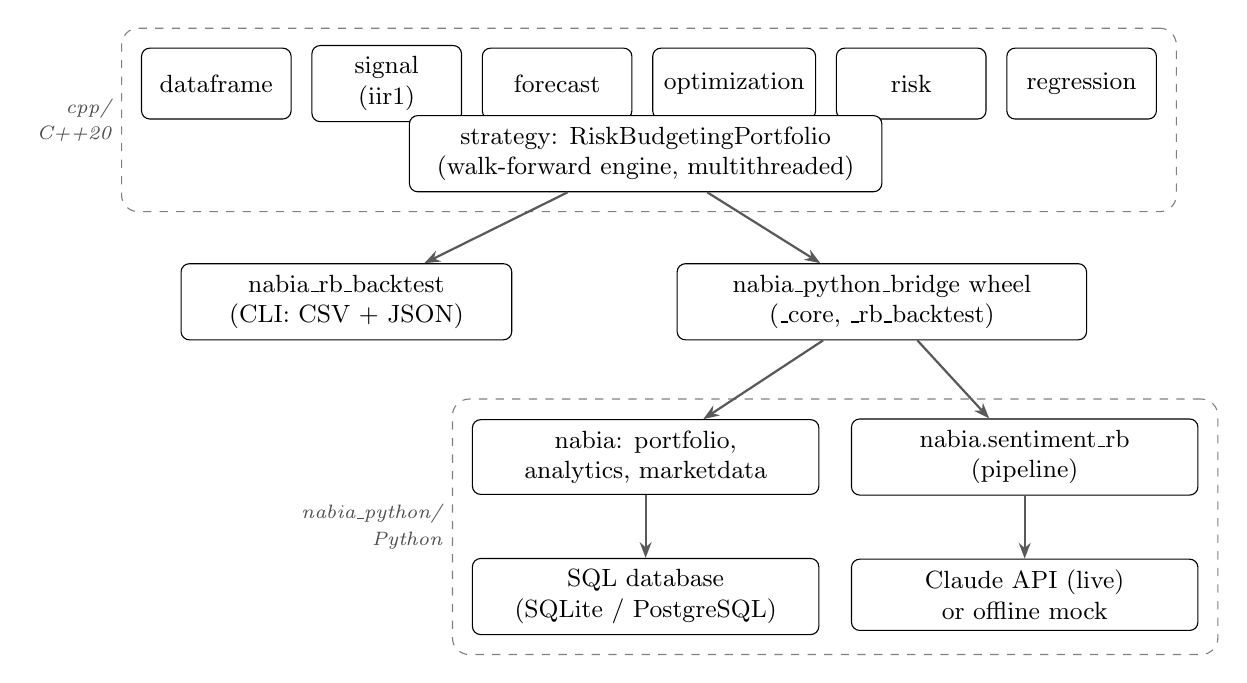
\begin{tikzpicture}[
  box/.style={draw, rounded corners=3pt, align=center, minimum height=9mm, font=\small, fill=white, inner sep=4pt},
  layer/.style={draw, dashed, rounded corners=6pt, inner sep=7pt, gray},
  arrow/.style={-{Stealth[length=2mm]}, thick, gray!70!black},
  lbl/.style={font=\scriptsize\itshape, gray!60!black}]
  \node[box, minimum width=19mm] (df) {dataframe};
  \node[box, right=2.5mm of df, minimum width=19mm] (sig) {signal\\(iir1)};
  \node[box, right=2.5mm of sig, minimum width=19mm] (fc) {forecast};
  \node[box, right=2.5mm of fc, minimum width=19mm] (opt) {optimization};
  \node[box, right=2.5mm of opt, minimum width=19mm] (risk) {risk};
  \node[box, right=2.5mm of risk, minimum width=19mm] (reg) {regression};
  \node[box, below=4mm of $(fc)!0.5!(opt)$, minimum width=60mm] (strat) {strategy: RiskBudgetingPortfolio\\(walk-forward engine, multithreaded)};
  \node[layer, fit=(df)(reg)(strat), label={[lbl]left:\shortstack[r]{cpp/\\C++20}}] (core) {};
  \node[box, below=9mm of strat, xshift=-38mm, minimum width=42mm] (cli) {nabia\_rb\_backtest\\(CLI: CSV + JSON)};
  \node[box, below=9mm of strat, xshift=30mm, minimum width=52mm] (bind) {nabia\_python\_bridge wheel\\(\_core, \_rb\_backtest)};
  \node[box, below=10mm of bind, xshift=-30mm, minimum width=44mm] (pkg) {nabia: portfolio,\\analytics, marketdata};
  \node[box, right=4mm of pkg, minimum width=44mm] (rb) {nabia.sentiment\_rb\\(pipeline)};
  \node[box, below=8mm of rb, minimum width=44mm] (llm) {Claude API (live)\\or offline mock};
  \node[box, below=8mm of pkg, minimum width=44mm] (db) {SQL database\\(SQLite / PostgreSQL)};
  \node[layer, fit=(pkg)(rb)(llm)(db), label={[lbl]left:\shortstack[r]{nabia\_python/\\Python}}] (py) {};
  \draw[arrow] (strat) -- (cli);
  \draw[arrow] (strat) -- (bind);
  \draw[arrow] (bind) -- (pkg);
  \draw[arrow] (bind) -- (rb);
  \draw[arrow] (rb) -- (llm);
  \draw[arrow] (pkg) -- (db);
\end{tikzpicture}
\caption{Components and dependencies. Arrows point from a component to what uses it.}
\label{fig:architecture}
\end{figure}

\begin{description}
  \item[C++ library] (\code{cpp/include/nabia}, \code{cpp/src}): the static library \code{nabia::nabia}, built with
        CMake, in C++20, on Eigen (linear algebra) and iir1 (filter design). Each module exposes an abstract
        interface whose parameter struct is owned through \code{std::unique\_ptr}: \code{IFilter<P>}
        (\coderef{ifilter}), \code{IForecaster<P>} (\coderef{iforecaster}), \code{IOptimizer<P,R>}
        (\coderef{ioptimizer}), \code{IRiskMeasure} (\coderef{irisk}). Part~\ref{part:core} describes every
        method, Part~\ref{part:derivations} derives the forecasters, the optimizers and the elastic net.
  \item[Application] \code{nabia\_rb\_backtest} (\code{cpp/apps/rb\_backtest}): a risk-budgeting backtest from a
        prices CSV and a JSON configuration (Chapter~\ref{c:sec:cli}).
  \item[Bindings] (\code{cpp/bindings}): one Python package, \code{nabia\_python\_bridge}, with two pybind11
        modules: \code{\_core} (the whole library) and \code{\_rb\_backtest} (the application's JSON backtest).
        \code{cpp/pyproject.toml} builds them into a wheel per Python version and platform
        (Chapters~\ref{c:sec:bridge}--\ref{ch:packaging}).
  \item[Python package] (\code{nabia\_python/nabia}): \code{nabia.backtest} and \code{nabia.latest\_weights} on
        pandas data (Chapter~\ref{p:sec:bindings}), analytics (Chapter~\ref{p:sec:stats}), market data
        (Chapter~\ref{p:sec:marketdata}), and the sentiment risk-budgeting pipeline \code{nabia.sentiment\_rb}
        (Part~\ref{part:sentiment}).
\end{description}

\section{Directory map}
\begin{center}\small
\begin{tabularx}{\linewidth}{@{}>{\raggedright\arraybackslash}p{5.2cm}>{\raggedright\arraybackslash}X@{}}
\toprule
Path & Contents \\
\midrule
\nolinkurl{cpp/include/nabia/dataframe} & \code{TimeSeries}, \code{DataFrame}, the \code{TimeIndex} concept \\
\nolinkurl{cpp/include/nabia/signal} & \code{IFilter}, \code{EWMA}, \code{ButterworthBandPass}, smoothing helpers \\
\nolinkurl{cpp/include/nabia/forecast} & \code{IForecaster}, SES, Kalman filter, Gaussian process, kernels \\
\nolinkurl{cpp/include/nabia/optimization} & \code{IOptimizer}; \code{convex/}: constraints, L-BFGS, augmented Lagrangian, SQP; \code{nongradopt/}: Nelder--Mead, differential evolution \\
\nolinkurl{cpp/include/nabia/risk} & \code{IRiskMeasure}, volatility, VaR, ES, \code{RiskBudgeting<Measure>} \\
\nolinkurl{cpp/include/nabia/stats, strategy, regression} & statistics; the portfolio engine and metrics; elastic net and the regression engine \\
\nolinkurl{cpp/src, cpp/tests} & implementations (same layout); Catch2 tests \\
\nolinkurl{cpp/apps/rb_backtest} & the command-line backtest \\
\nolinkurl{cpp/bindings} & pybind11 sources (\code{src}) and the Python files of the wheel (\code{nabia\_python\_bridge}) \\
\nolinkurl{cpp/pyproject.toml, cpp/scripts} & wheel build (scikit-build-core, cibuildwheel), \code{build\_wheels.sh}, \code{.ps1} \\
\nolinkurl{nabia_python/nabia} & \code{portfolio.py}, \code{analytics.py}, \code{marketdata/}, \code{sentiment\_rb/} \\
\nolinkurl{nabia_python/nabia/sentiment_rb} & \code{config.py}, \code{pipeline.py}, \code{\_\_main\_\_.py}; \code{data/}, \code{features/}, \code{llm/}, \code{model/}, \code{portfolio/}, \code{report/}, \code{prompts/} \\
\nolinkurl{nabia_python/tests, scripts} & pytest suites (\code{tests/bridge} tests the wheel); \code{setup\_env}, \code{fetch\_wheels} \\
\nolinkurl{doc} & this document and the pipeline's specification \\
\bottomrule
\end{tabularx}
\end{center}

\section{Build and test summary}
\begin{center}\small
\begin{tabularx}{\linewidth}{@{}l X@{}}
\toprule
Task & Command (Chapter~\ref{ch:guide}) \\
\midrule
C++ build and tests & \code{cd cpp \&\& cmake --preset debug \&\& cmake --build --preset debug \&\& ctest --preset debug} \\
Wheels & \code{cpp/scripts/build\_wheels.sh [versions]}; CI: \code{gh workflow run wheels.yml} \\
Python environment and tests & \code{nabia\_python/scripts/setup\_env.sh}; \code{cd nabia\_python \&\& .venv/bin/python -m pytest} \\
Pipeline & \code{.venv/bin/python -m nabia.sentiment\_rb [--config c.json] [--ic-sweep ...]} \\
This document & \code{doc/build.sh [--figures]} \\
\bottomrule
\end{tabularx}
\end{center}


\part{The numerical core (C++)}\label{part:core}
% The numerical core (C++): containers, filters, forecasters, optimizers, risk, the portfolio engine,
% metrics and the regression engine. Excerpts and locations come from extract_snippets.py.

\chapter{Time series containers}\label{c:sec:dataframe}

All numerical code works on Eigen matrices, but financial data is indexed by time.
\code{TimeSeries<Index>} and \code{DataFrame<Index>} pair an Eigen vector or matrix (rows
are times) with a \emph{strictly increasing} index:
\begin{itemize}
  \item The index type satisfies the \code{TimeIndex} concept (copyable and totally
        ordered): calendar dates, timestamps or integers.
  \item Construction validates the shapes, the ordering and unique column names.
  \item Time lookups use binary search.
\end{itemize}

\paragraph{Alignment.} Markets have different holidays. A cross-asset backtest keeps only
the dates where every asset has a finite price.

\paragraph{Returns.} Simple returns $r_t=P_t/P_{t-1}-1$ (\code{pct\_change}) or log returns
$\log(P_t/P_{t-1})$ are computed between consecutive \emph{kept} rows. A return can
therefore span a removed holiday. That is the right convention for a portfolio that can
only trade when all its markets are open.

\snippet{df_drop_missing}{C++}{Alignment: keep rows where every column is finite}
\begin{codepointers}
  \codeitem{time_index}{\code{TimeIndex} concept}
  \codeitem{timeseries}{\code{TimeSeries}}
  \codeitem{dataframe}{\code{DataFrame}}
  \codeitem{pct_change}{simple returns}
  \codeitem{log_returns}{log returns}
\end{codepointers}

\chapter{Signal extraction}\label{c:sec:signal}

Filters implement \code{IFilter<P>}. They are \emph{causal}: output $t$ uses inputs up to
$t$ only. Two modes are supported:
\begin{itemize}
  \item streaming: \code{process(x)}, one sample at a time, keeping state;
  \item batch: \code{apply(signal)}, from a fresh state, without disturbing the streaming
        state.
\end{itemize}
Filter design is delegated to iir1, behind a private implementation struct (pimpl), so iir1
never appears in public headers.

\section{Exponentially weighted moving average}
The EWMA is the one-pole low-pass
\[
  y_t=\alpha x_t+(1-\alpha)y_{t-1},\qquad H(z)=\frac{\alpha}{1-(1-\alpha)z^{-1}},\qquad \alpha\in(0,1].
\]
Its DC gain is $H(1)=1$, so a constant input passes unchanged.

\begin{proposition}[Seeding]
Let $\tilde y$ be the EWMA of $x_t-x_0$ started from a zero state. Then $y_t=x_0+\tilde y_t$
equals the recursion started at $y_{-1}=x_0$:
\[
  y_t=\alpha\sum_{k=0}^{t}(1-\alpha)^k x_{t-k}+(1-\alpha)^{t+1}x_0 .
\]
\end{proposition}
\begin{proof}
Unrolling the recursion from $y_{-1}$ gives
$y_t=\alpha\sum_{k=0}^{t}(1-\alpha)^kx_{t-k}+(1-\alpha)^{t+1}y_{-1}$. With a zero state,
$\tilde y_t=\alpha\sum_{k=0}^t(1-\alpha)^k(x_{t-k}-x_0)$. Using
$\alpha\sum_{k=0}^t(1-\alpha)^k=1-(1-\alpha)^{t+1}$, adding $x_0$ gives the formula with
$y_{-1}=x_0$.
\end{proof}
Starting from zero instead would bias the early outputs towards zero, so the filter seeds
with the first sample by default.

\paragraph{Parameterizations.} Two helpers convert the usual parameterizations to $\alpha$:
\begin{itemize}
  \item \code{alpha\_from\_span}$(N)=2/(N+1)$. The mean age of the EWMA weights is
        $\sum_k k\,\alpha(1-\alpha)^k=(1-\alpha)/\alpha$, and that of an $N$-point moving
        average is $(N-1)/2$. Equating the two gives $\alpha=2/(N+1)$.
  \item \code{alpha\_from\_halflife}$(h)=1-2^{-1/h}$. This solves $(1-\alpha)^h=\tfrac12$:
        the weight $h$ steps back is half the newest weight.
\end{itemize}

\snippet{ewma_impl}{C++}{EWMA on iir1's one-pole section, with first-sample seeding}
\begin{codepointers}
  \codeitem{ewma_class}{class and parameters}
  \codeitem{ewma_alphas}{span and half-life conversions}
  \codeitem{moving_average}{simple moving average helper (rolling sum, $O(n)$)}
\end{codepointers}

\section{Butterworth band-pass}
A causal Butterworth band-pass isolates trend cycles between two frequencies
$0<f_\ell<f_h<f_s/2$. It is built in three steps.
\begin{enumerate}
  \item \textbf{Analog prototype.} The order-$N$ low-pass prototype is maximally flat:
        \[
          |H(j\Omega)|^2=\frac{1}{1+\Omega^{2N}},
        \]
        with poles $s_k=e^{j\pi(2k+N-1)/(2N)}$, $k=1,\dots,N$, on the left half of the unit
        circle.
  \item \textbf{Low-pass to band-pass.} The substitution
        \[
          s\mapsto\frac{s^2+\Omega_0^2}{sB}
        \]
        maps it to a band-pass with $2N$ poles, centred on $\Omega_0$ with bandwidth $B$.
  \item \textbf{Bilinear transform.} The map $s=2f_s\frac{1-z^{-1}}{1+z^{-1}}$, with the band
        edges prewarped by $\Omega=2f_s\tan(\pi f/f_s)$, gives the digital filter. It is run
        as a cascade of second-order sections, which is numerically stable at high orders.
\end{enumerate}
iir1 takes the band as a centre and a width, so the edges map to centre
$(f_\ell+f_h)/2$ and width $f_h-f_\ell$. The filter then has $|H|=1/\sqrt2$ ($-3$\,dB)
at both edges and unit gain at the centre. The tests check exactly these properties, and
strong attenuation outside the band. Being causal, the filter delays the signal: the
group delay grows with the order and with narrower bands.
\begin{codepointers}
  \codeitem{butterworth_params}{parameters (order, sample rate, edges)}
  \codeitem{butterworth_design}{design: edges to centre and width}
\end{codepointers}

\chapter{Forecasting}\label{c:sec:forecast}

Forecasters implement \code{IForecaster<P>}:
\begin{itemize}
  \item \code{fit(y)} estimates the model on a series;
  \item \code{forecast(H)} returns the mean $\hat y_{T+h}$ and the predictive variance $v_h$
        for $h=1..H$;
  \item Gaussian prediction intervals follow as $\hat y\pm z_{(1+c)/2}\sqrt{v_h}$.
\end{itemize}
Chapters~\ref{ch:es}--\ref{ch:gp} derive each model in full. This section states
what the code computes.

\section{Simple exponential smoothing}
The model is the ETS(A,N,N) state space
\[
  y_t=\ell_{t-1}+\varepsilon_t,\qquad \ell_t=\ell_{t-1}+\alpha\varepsilon_t,\qquad
  \varepsilon_t\sim\N(0,\sigma^2).
\]
The fit initializes $\ell=y_1$ and runs the error-correction form
$\ell\leftarrow\ell+\alpha(y_t-\ell)$, accumulating $\mathrm{SSE}=\sum_t(y_t-\ell_{t-1})^2$.
It then estimates $\hat\sigma^2=\mathrm{SSE}/T$.

\begin{proposition}
The $h$-step forecast is $\hat y_{T+h}=\ell_T$, with variance $\sigma^2\big(1+(h-1)\alpha^2\big)$.
\end{proposition}
\begin{proof}
Iterating the state equation gives $\ell_{T+h-1}=\ell_T+\alpha\sum_{j=1}^{h-1}\varepsilon_{T+j}$,
so $y_{T+h}=\ell_T+\alpha\sum_{j=1}^{h-1}\varepsilon_{T+j}+\varepsilon_{T+h}$. The errors are
independent, so the variance is $(h-1)\alpha^2\sigma^2+\sigma^2$.
\end{proof}
\snippet{ses_fit}{C++}{SES fit and forecast variance}

\section{Kalman filter}
The model is the linear Gaussian state space
\[
  x_t=Fx_{t-1}+w_t,\quad w_t\sim\N(0,Q);\qquad y_t=Hx_t+v_t,\quad v_t\sim\N(0,R),
\]
with prior $x_0\sim\N(\hat x_0,P_0)$, where the prior describes the first state. Each step
first predicts:
\[
  \hat x_{t|t-1}=F\hat x_{t-1|t-1},\qquad P_{t|t-1}=FP_{t-1|t-1}F^\T+Q .
\]
Then it computes the innovation and its variance:
\[
  e_t=y_t-H\hat x_{t|t-1},\qquad S_t=HP_{t|t-1}H^\T+R .
\]
Finally it corrects, with gain $K_t=P_{t|t-1}H^\T/S_t$:
\[
  \hat x_{t|t}=\hat x_{t|t-1}+K_te_t,\qquad
  P_{t|t}=(I-K_tH)P_{t|t-1}(I-K_tH)^\T+R\,K_tK_t^\T .
\]
\begin{itemize}
  \item \textbf{Joseph form.} The covariance update above is the posterior covariance for
        \emph{any} gain. It is symmetric and positive semi-definite by construction, so it
        stays valid under rounding, unlike the short form $(I-KH)P$.
  \item \textbf{Missing observations.} Non-finite $y_t$ skip the correction.
  \item \textbf{Log-likelihood.}
        $\ell=-\tfrac12\sum_t\big(\log2\pi+\log S_t+e_t^2/S_t\big)$, summed over the observed
        points.
  \item \textbf{Forecasts.} They iterate the prediction step: mean $Hx$, variance
        $HPH^\T+R$.
  \item \textbf{Smoothing.} The Rauch--Tung--Striebel smoother uses the gain
        $C_t=P_{t|t}F^\T P_{t+1|t}^{-1}$ (computed by an $LDL^\T$ solve, not an inverse) and
        $\hat x^s_t=\hat x_{t|t}+C_t(\hat x^s_{t+1}-\hat x_{t+1|t})$.
\end{itemize}

Two ready-made models are provided:
\begin{itemize}
  \item \emph{local level}: $F=H=1$, so the level is a random walk observed with noise;
  \item \emph{local linear trend}: $F=\begin{psmallmatrix}1&1\\0&1\end{psmallmatrix}$,
        $H=(1,0)$, $Q=\diag(q_\ell,q_s)$, so level and slope both drift.
\end{itemize}
Both use a diffuse prior ($P_0=10^7I$). The local linear trend's slope state is a direct
estimate of the trend.
\snippet{kalman_step}{C++}{Kalman predict and Joseph-form correction}
\begin{codepointers}
  \codeitem{kalman_params}{parameters $F,H,Q,R,x_0,P_0$}
  \codeitem{kalman_models}{local level and local linear trend}
  \codeitem{kalman_forecast}{forecast}
  \codeitem{kalman_smoother}{RTS smoother}
\end{codepointers}

\section{Gaussian process regression}
The series is regressed on time $t=0,\dots,T-1$ in three steps.
\begin{enumerate}
  \item \textbf{Standardization.} The observations are standardized,
        $z=(y-\bar y)/s$, where $s$ is the sample standard deviation when normalizing.
  \item \textbf{Model.} $z\sim\N(0,K)$ with $K=K_f+\sigma_n^2I$ and
        $(K_f)_{ij}=k(t_i,t_j)$. The available kernels, with $r=t-t'$:
\begin{align*}
  k_{\text{SE}}&=\sigma^2\exp\!\big(-r^2/2\ell^2\big),\\
  k_{\text{M52}}&=\sigma^2\big(1+u+u^2/3\big)e^{-u},\quad u=\sqrt5|r|/\ell,\\
  k_{\text{per}}&=\sigma^2\exp\!\big(-2\sin^2(\pi r/p)/\ell^2\big).
\end{align*}
        Sums and products of kernels are kernels too.
  \item \textbf{Hyperparameters.} With $\alpha=K^{-1}z$ (from a Cholesky factorization
        $K=LL^\T$), the log marginal likelihood is
\[
  \log p(z)=-\tfrac12z^\T\alpha-\textstyle\sum_i\log L_{ii}-\tfrac T2\log2\pi .
\]
        The hyperparameters $\theta$ (logs of variances, length scales, periods and,
        optionally, the noise) maximize it, using L-BFGS with the analytic gradient
\[
  \frac{\partial(-\log p)}{\partial\theta_j}=-\tfrac12\tr\!\Big(\big(\alpha\alpha^\T-K^{-1}\big)\frac{\partial K}{\partial\theta_j}\Big).
\]
        Working in logs keeps the parameters positive. Values with $|\theta_j|>20$, or a
        $K$ that is not positive definite, are returned as $+\infty$, which the line search
        rejects. The noise has a floor (\code{min\_noise\_variance}).
\end{enumerate}

\paragraph{Prediction.} At new times $t_*$, with $v=L^{-1}k_*$:
\[
  \text{mean}=\bar y+s\,k_*^\T\alpha,\qquad
  \text{variance}=s^2\big(k(t_*,t_*)-v^\T v+\sigma_n^2\big).
\]
The reported likelihood is converted back to the units of $y$ by subtracting $T\log s$.
\snippet{gp_nll}{C++}{Gaussian process: negative log-likelihood gradient}
\begin{codepointers}
  \codeitem{gp_factorize}{Cholesky and log marginal likelihood}
  \codeitem{gp_fit}{fit with hyperparameter optimization}
  \codeitem{gp_predict}{predictive mean and variance}
  \codeitem{kernels}{kernels and their log-parameter gradients}
\end{codepointers}

\chapter{Optimization}\label{c:sec:optimization}

Optimizers implement \code{IOptimizer<P,R>}: \code{optimize(initial\_guess)} returns the
solution, and \code{result()} returns a solver-specific result object (status, iterations,
residuals). Linear constraints are expressed in matrix form:
$A_{\text{eq}}x=b_{\text{eq}}$ and $A_{\text{in}}x\le b_{\text{in}}$. Box bounds
$l\le x\le u$ convert to inequality rows.
\begin{codepointers}
  \codeitem{ioptimizer}{optimizer interface}
  \codeitem{constraints}{linear constraints and their conversion}
\end{codepointers}

\section{L-BFGS}\label{c:sec:lbfgs}
L-BFGS minimizes a smooth $f$ with search direction $d=-H_kg_k$. Here $H_k$ is the BFGS
inverse-Hessian approximation built from the last $m$ pairs
$s_j=x_{j+1}-x_j$, $y_j=g_{j+1}-g_j$, with $\rho_j=1/s_j^\T y_j$. It is applied in $O(mn)$
by the two-loop recursion:
\begin{enumerate}
  \item $q\leftarrow g$. For $j$ from newest to oldest: $a_j=\rho_js_j^\T q$, then
        $q\leftarrow q-a_jy_j$.
  \item $r\leftarrow\gamma q$, with $\gamma=s^\T y/y^\T y$ from the newest pair. On the
        first iteration $\gamma=1/\max(1,\norm{g})$.
  \item For $j$ from oldest to newest: $\beta=\rho_jy_j^\T r$, then
        $r\leftarrow r+(a_j-\beta)s_j$. Finally $d=-r$.
\end{enumerate}
Safeguards keep the method well defined:
\begin{itemize}
  \item A pair is stored only if $s^\T y>10^{-12}\norm s\norm y$ (the curvature
        condition), which keeps $H$ positive definite.
  \item If $d$ is not a descent direction, the memory is cleared and the method restarts
        from steepest descent.
  \item Iteration stops when $\norm{g}_\infty\le\varepsilon$.
\end{itemize}

\paragraph{Line search.} Backtracking from $t=1$ halves $t$ until the step is accepted. A
non-finite $f$ counts as rejection, which is how barrier and domain constraints are
enforced. A step is accepted under either condition:
\begin{description}
  \item[Armijo] $f(x+td)\le f(x)+c_1t\,g^\T d$, with $c_1=10^{-4}$.
  \item[Approximate Wolfe] (Hager--Zhang), when $f$ is flat to within rounding:
        $f(x+td)\le f(x)+\epsilon_f|f(x)|$ and
        $\sigma\,g^\T d\le g(x+td)^\T d\le(2c_1-1)\,g^\T d$, with $\epsilon_f=10^{-10}$ and
        $\sigma=0.9$.
\end{description}
Near a minimum the decrease Armijo requires is smaller than the rounding error in $f$,
while directional derivatives remain accurate. The second test lets the method keep
converging there. On 500-asset risk budgeting it took the attainable budget accuracy from
about $3\cdot10^{-8}$ to $10^{-8}$.
\snippet{lbfgs_two_loop}{C++}{Two-loop recursion}
\snippet{lbfgs_line_search}{C++}{Line search: Armijo or approximate Wolfe}
\begin{codepointers}
  \codeitem{lbfgs_params}{parameters and defaults}
  \codeitem{lbfgs_optimize}{full algorithm}
\end{codepointers}

\section{Augmented Lagrangian}\label{c:sec:al}
For $\min f(x)$ subject to $h(x)=A_{\text{eq}}x-b_{\text{eq}}=0$ and
$g(x)=A_{\text{in}}x-b_{\text{in}}\le0$, the Powell--Hestenes--Rockafellar augmented
Lagrangian is
\[
  L_\rho(x;\lambda,\mu)=f(x)+\lambda^\T h+\frac\rho2\norm h^2
  +\frac1{2\rho}\sum_i\Big(\max(0,\mu_i+\rho g_i)^2-\mu_i^2\Big),
\]
with gradient
$\nabla f+A_{\text{eq}}^\T(\lambda+\rho h)+A_{\text{in}}^\T\max(0,\mu+\rho g)$.
Each outer iteration does four things:
\begin{enumerate}
  \item \textbf{Minimize} $L_\rho$ with L-BFGS, warm-started at the previous iterate. The
        inner tolerance starts at $\max(\varepsilon,0.1)$ and shrinks tenfold per outer
        iteration down to $\varepsilon$.
  \item \textbf{Measure} the violation
        $v=\max\big(\norm h_\infty,\norm{\max(g,-\mu/\rho)}_\infty\big)$. The second term is
        zero if and only if $g\le0$ and $\mu_ig_i=0$, so it also measures complementarity.
  \item \textbf{Update the multipliers}: $\lambda\leftarrow\lambda+\rho h$ and
        $\mu\leftarrow\max(0,\mu+\rho g)$. After this update,
        $\nabla_xL_\rho=\nabla f+A_{\text{eq}}^\T\lambda+A_{\text{in}}^\T\mu$, so the inner
        gradient norm is the KKT stationarity.
  \item \textbf{Test and adapt.} Stop when $v\le\varepsilon$ and stationarity
        $\le\varepsilon$. Otherwise, if $v>0.25\,v_{\text{prev}}$, set
        $\rho\leftarrow\min(10\rho,10^{10})$ (starting from $\rho_0=10$).
\end{enumerate}
\snippet{al_function}{C++}{Augmented Lagrangian value and gradient}
\snippet{al_updates}{C++}{Multiplier and penalty updates}
\begin{codepointers}
  \codeitem{al_options}{options and defaults}
  \codeitem{al_optimize}{full algorithm}
\end{codepointers}

\section{Sequential quadratic programming}
At $x_k$, SQP solves the quadratic subproblem
\[
  \min_d\;g_k^\T d+\tfrac12d^\T B_kd\quad\text{s.t.}\quad
  A_{\text{eq}}d=b_{\text{eq}}-A_{\text{eq}}x_k,\;\;A_{\text{in}}d\le b_{\text{in}}-A_{\text{in}}x_k .
\]
It uses the augmented Lagrangian of \S\ref{c:sec:al} at tolerance $10^{-10}$, or a Cholesky
solve $d=-B^{-1}g$ when there are no constraints.
\begin{description}
  \item[Convergence] is declared when three KKT residuals at $x_k$, computed with the QP
        multipliers, are all below $\varepsilon$:
        \begin{itemize}
          \item stationarity
                $\norm{g+A_{\text{eq}}^\T\lambda+A_{\text{in}}^\T\mu}_\infty$;
          \item constraint violation;
          \item complementarity $\max_i|\mu_ig_i|$.
        \end{itemize}
  \item[Merit function] $\phi(x)=f(x)+\nu V_1(x)$, with
        $V_1=\norm h_1+\sum_i\max(g_i,0)$. The penalty is kept at
        $\nu\ge\norm{(\lambda,\mu)}_\infty+10^{-3}$. Because the constraints are linear and
        $d$ satisfies the linearized constraints, $V_1(x+td)\le(1-t)V_1(x)$. The
        directional derivative is therefore bounded by $g^\T d-\nu V_1(x)<0$, so $d$
        descends $\phi$. Backtracking applies Armijo to $\phi$ with this slope.
  \item[Restart] If the line search fails, $B$ resets to the identity. A failure from
        $B=I$ ends the iteration.
\end{description}

\begin{proposition}[Damped BFGS, Powell]
Let $r=\theta y+(1-\theta)Bs$, with $\theta=1$ if $s^\T y\ge0.2\,s^\T Bs$ and
$\theta=0.8\,s^\T Bs/(s^\T Bs-s^\T y)$ otherwise. The update
\[
  B^+=B-\frac{Bss^\T B}{s^\T Bs}+\frac{rr^\T}{s^\T r}
\]
keeps $B$ positive definite.
\end{proposition}
\begin{proof}
If $\theta<1$, then $s^\T r=s^\T Bs-\theta(s^\T Bs-s^\T y)=0.2\,s^\T Bs>0$. If $\theta=1$,
then $s^\T r=s^\T y\ge0.2\,s^\T Bs>0$. The BFGS update with a pair satisfying $s^\T r>0$
preserves positive definiteness.
\end{proof}
After the first step with $s^\T y>0$, $B$ is scaled to $(y^\T y/s^\T y)I$ before the update,
which matches the curvature along $s$.
\snippet{sqp_bfgs}{C++}{Damped BFGS update}
\snippet{sqp_merit}{C++}{$\ell_1$ merit penalty and line search}
\begin{codepointers}
  \codeitem{sqp_options}{options and defaults}
  \codeitem{sqp_qp}{QP subproblem through the augmented Lagrangian}
  \codeitem{sqp_optimize}{full algorithm}
\end{codepointers}

\section{Nelder--Mead with box bounds}
Nelder--Mead keeps a simplex of $n+1$ vertices sorted by value,
$f(x_0)\le\dots\le f(x_n)$, with $c$ the centroid of the best $n$. Each iteration:
\begin{enumerate}
  \item \textbf{Reflect}: $x_r=c+\alpha(c-x_n)$.
  \item If $f_r<f_0$, \textbf{expand} to $x_e=c+\gamma(x_r-c)$ and keep the better of
        $x_e$ and $x_r$.
  \item Else, if $f_r<f_{n-1}$, accept $x_r$.
  \item Else \textbf{contract}:
        \begin{itemize}
          \item outside, $x_c=c+\rho(x_r-c)$, if $f_r<f_n$ (accepted if $f_c<f_r$);
          \item inside, $x_c=c+\rho(x_n-c)$, otherwise (accepted if $f_c<f_n$).
        \end{itemize}
  \item Else \textbf{shrink} every vertex towards the best:
        $x_j\leftarrow x_0+\sigma(x_j-x_0)$.
\end{enumerate}
The \emph{adaptive} coefficients of Gao and Han, $\alpha=1$, $\gamma=1+2/n$,
$\rho=\tfrac34-\tfrac1{2n}$, $\sigma=1-\tfrac1n$, avoid the stagnation of the standard
values $(1,2,\tfrac12,\tfrac12)$ in higher dimensions.

Bounds are enforced by projecting every trial point onto the box. The box is convex, so a
shrink stays inside it.

\paragraph{Termination.} The iteration stops when both conditions hold:
\[
  f_n-f_0\le\tau_f(1+|f_0|)\quad\text{and}\quad\max_j\norm{x_j-x_0}_\infty\le\tau_x(1+\norm{x_0}_\infty).
\]
A NaN objective counts as $+\infty$.
\snippet{nm_step}{C++}{One Nelder--Mead iteration}
\begin{codepointers}
  \codeitem{nm_coefficients}{adaptive coefficients}
  \codeitem{box}{box projection}
  \codeitem{nm_optimize}{full algorithm, initial simplex}
\end{codepointers}

\section{Differential evolution}
\paragraph{Population.} $N_p$ vectors (default $15n$, at least 4, or 6 for rand/2), drawn
uniformly in the box. An initial guess, if given, replaces member 0.

\paragraph{Mutation.} Each generation draws one $F\sim U[F_{\min},F_{\max}]$ (dithering),
then builds a mutant per member $i$ from distinct random members $r_1,\dots,r_5\ne i$:
\begin{align*}
  \text{rand/1:}\quad& v=x_{r_1}+F(x_{r_2}-x_{r_3}),\\
  \text{best/1:}\quad& v=x_{\text{best}}+F(x_{r_1}-x_{r_2}),\\
  \text{current-to-best/1:}\quad& v=x_i+F(x_{\text{best}}-x_i)+F(x_{r_1}-x_{r_2}),\\
  \text{rand/2:}\quad& v=x_{r_1}+F(x_{r_2}-x_{r_3})+F(x_{r_4}-x_{r_5}).
\end{align*}

\paragraph{Crossover.} Binomial: $u_{ij}=v_{ij}$ if $U<\mathrm{CR}$ or $j=j_{\text{rand}}$,
else $x_{ij}$, so at least one coordinate comes from the mutant. A coordinate outside the
box bounces back to the midpoint between the parent and the violated bound.

\paragraph{Selection.} Greedy: $u$ replaces $x_i$ if $f(u)\le f(x_i)$. Ties go to the trial,
which keeps the population moving on plateaus.

\paragraph{Termination.} The run stops when the population's objective values have
$\mathrm{sd}(f)\le\tau_a+\tau|\overline f|$.

\paragraph{Parallelism and reproducibility.} All trial vectors of a generation are built
sequentially from one seeded RNG \emph{before} evaluation. Only the evaluations run in
parallel, so the result is the same for every thread count. A \code{ParallelEvaluator<T,R>}
does the evaluations:
\begin{itemize}
  \item each input becomes a \code{std::packaged\_task} in a queue;
  \item $n$ worker threads consume the queue;
  \item the caller collects the results, in input order, through the tasks' futures.
\end{itemize}
\snippet{de_generation}{C++}{Mutation and crossover of one generation}
\snippet{parallel_evaluator}{C++}{ParallelEvaluator: job queue, consumers, futures}
\begin{codepointers}
  \codeitem{de_params}{parameters and defaults}
  \codeitem{de_optimize}{full algorithm}
\end{codepointers}

\chapter{Risk measures}\label{c:sec:risk}

For portfolio weights $x$ on assets with return covariance $\Sigma$ and mean $\mu$, write
$\sigma(x)=\sqrt{x^\T\Sigma x}$ and take the loss $L=-r^\T x$ with $r\sim\N(\mu,\Sigma)$. Then
$L\sim\N(-\mu^\T x,\sigma(x)^2)$. The three measures are:
\begin{align*}
  \text{Volatility:}\quad & R(x)=\sigma(x), & \nabla R &= \Sigma x/\sigma(x),\\
  \text{VaR}_\alpha:\quad & R(x)=-\mu^\T x+z_\alpha\,\sigma(x), & \nabla R&=-\mu+z_\alpha\Sigma x/\sigma(x),\\
  \text{ES}_\alpha:\quad & R(x)=-\mu^\T x+\frac{\varphi(z_\alpha)}{1-\alpha}\,\sigma(x), & \nabla R&=-\mu+\frac{\varphi(z_\alpha)}{1-\alpha}\Sigma x/\sigma(x),
\end{align*}
with $z_\alpha=\Phi^{-1}(\alpha)$.

\begin{proposition}[Gaussian expected shortfall]
If $L\sim\N(m,s^2)$, then
$\mathrm{ES}_\alpha=\E[L\mid L\ge\mathrm{VaR}_\alpha]=m+s\,\varphi(z_\alpha)/(1-\alpha)$.
\end{proposition}
\begin{proof}
Write $L=m+sZ$. The event is $Z\ge z_\alpha$, which has probability $1-\alpha$. Since
$\varphi'(z)=-z\varphi(z)$, we get $\int_{z_\alpha}^\infty z\varphi(z)\,dz=\varphi(z_\alpha)$,
so $\E[Z\mid Z\ge z_\alpha]=\varphi(z_\alpha)/(1-\alpha)$.
\end{proof}

\begin{proposition}[Euler decomposition]
Each measure is positively homogeneous of degree one, $R(cx)=cR(x)$ for $c>0$. Hence
$R(x)=\sum_ix_i\,\partial_iR(x)$, and the \emph{risk contributions}
$\mathrm{RC}_i=x_i\partial_iR$ add up exactly to the total risk.
\end{proposition}
\begin{proof}
Differentiate $R(cx)=cR(x)$ with respect to $c$ at $c=1$.
\end{proof}
At $\sigma=0$ the gradient of $\sigma$ is set to zero, which is a valid subgradient of the
seminorm. The quantile $\Phi^{-1}$ uses Acklam's rational approximation (relative error
below $1.2\cdot10^{-9}$), refined to full precision by one Halley step on $\Phi(x)-p$:
\[
  x\leftarrow x-\frac{u}{1+xu/2},\qquad u=(\Phi(x)-p)\sqrt{2\pi}\,e^{x^2/2}.
\]
\snippet{vol_gradient}{C++}{Volatility gradient, the building block of every measure}
\snippet{var_measure}{C++}{Gaussian VaR and its gradient}
\begin{codepointers}
  \codeitem{irisk}{risk measure interface}
  \codeitem{risk_contributions}{risk contributions $x\odot\nabla R$}
  \codeitem{volatility_measure}{volatility}
  \codeitem{es_measure}{expected shortfall (constant $\varphi(z_\alpha)/(1-\alpha)$)}
  \codeitem{normal_quantile}{normal quantile: Halley refinement}
\end{codepointers}

\chapter{Risk budgeting}\label{c:sec:riskbudgeting}

Given budgets $b_i>0$ with $\sum_ib_i=1$, the \emph{risk budgeting portfolio} is the
long-only $x$ with $\mathrm{RC}_i(x)/R(x)=b_i$ for all $i$. Equal budgets give the equal risk
contribution portfolio.

\begin{theorem}\label{c:thm:rb}
Let $R$ be convex, positively homogeneous of degree one, differentiable on $y>0$, and
positive on $\{y\ge0,\,y\ne0\}$. Then
\[
  f(y)=R(y)-\sum_ib_i\log y_i
\]
has a unique minimizer $y^\ast>0$, and $x^\ast=y^\ast/\sum_iy^\ast_i$ is the unique long-only
portfolio with $\mathrm{RC}_i(x^\ast)/R(x^\ast)=b_i$. Moreover $R(y^\ast)=1$.
\end{theorem}
\begin{proof}
\emph{Existence.} $R$ is continuous and positive on the compact simplex
$\Delta=\{y\ge0,\sum y_i=1\}$, so $c=\min_\Delta R>0$. By homogeneity,
$R(y)\ge c\sum_iy_i$ for $y\ge0$. Hence $f(y)\ge\sum_i(cy_i-b_i\log y_i)$. Each term tends
to $+\infty$ as $y_i\to0^+$ or $y_i\to\infty$, so $f$ is coercive on $y>0$ and attains
its minimum.

\emph{Uniqueness.} $-\sum b_i\log y_i$ is strictly convex and $R$ is convex, so $f$ is
strictly convex.

\emph{Characterization.} At the minimizer, $\partial_if=\partial_iR(y^\ast)-b_i/y^\ast_i=0$,
so $\mathrm{RC}_i(y^\ast)=y^\ast_i\partial_iR(y^\ast)=b_i$. Summing and using Euler gives
$R(y^\ast)=\sum_ib_i=1$. Let $S=\sum_iy^\ast_i$. Because $\partial_iR$ is homogeneous of
degree zero, $x^\ast=y^\ast/S$ has $\mathrm{RC}_i(x^\ast)=b_i/S$ and $R(x^\ast)=1/S$, so
$\mathrm{RC}_i/R=b_i$.

Conversely, if $x$ satisfies the budget condition, then $y=x/R(x)$ satisfies
$\partial_if(y)=0$ and is therefore the unique minimizer.
\end{proof}

For VaR and ES, the condition ``$R>0$ on long-only portfolios'' needs
$z\,\sigma(x)>\mu^\T x$. The solver checks it at the start and throws otherwise.

\paragraph{Algorithm.} The steps follow \coderef{rb_solver}.
\begin{enumerate}
  \item \textbf{Normalize} the budgets. Empty budgets mean equal risk.
  \item \textbf{Start} at $y^0_i\propto b_i/\sigma_i$, scaled so that $R(y^0)=1$. That
        scale is the magnitude of the solution by the theorem. The start is the
        inverse-volatility portfolio for equal budgets, which is exact for uncorrelated
        assets.
  \item \textbf{Minimize} $f$ with L-BFGS (memory 20). Points with any $y_i\le0$ return
        $+\infty$, so the log barrier needs no explicit constraint.
  \item \textbf{Match the tolerance to the budget error.} L-BFGS stops on
        $\norm{\nabla f}_\infty$, but the target is the budget error
        $e=\max_i|\mathrm{RC}_i/R-b_i|$. Near the solution $R\approx1$ and
        $\mathrm{RC}_i-b_i=y_i\nabla_if$, so $e\lesssim\max_iy_i\,\norm{\nabla f}_\infty$.
        The inner tolerance therefore starts at $\tau/\max_iy^0_i$. If $e>\tau$ afterwards,
        L-BFGS warm-restarts with tolerance $\tau_{\text{in}}\cdot\tfrac12\tau/e$, at most five
        times.
  \item \textbf{Return} $x=y/\sum y$, with risk, contributions, budget error and a
        convergence flag.
\end{enumerate}
\snippet{rb_objective}{C++}{Objective and gradient, for any risk measure}
\snippet{rb_solve}{C++}{Tolerance matching on the budget error}
\begin{codepointers}
  \codeitem{rb_budgets}{budget normalization}
  \codeitem{rb_start}{starting point}
  \codeitem{rb_template}{\code{RiskBudgeting<Measure>} wrapper}
\end{codepointers}

\chapter{The walk-forward portfolio engine}\label{c:sec:engine}

\code{RiskBudgetingPortfolio} backtests a long-only risk budgeting portfolio from a
$T\times N$ matrix of simple returns, where row $t$ holds the returns over $(t-1,t]$.
Table~\ref{c:tab:portfolio} lists its parameters, which are also the JSON keys of the CLI and
the Python API.

\begin{table}[ht]\centering\small
\caption{Portfolio parameters: engine defaults and the defaults of the AI configuration.}
\label{c:tab:portfolio}
\begin{tabularx}{\linewidth}{@{}l l l X@{}}
\toprule
Key & Engine & AI & Meaning \\
\midrule
\code{covariance\_window} & 60 & 120 & rows $W$ per covariance estimate \\
\code{covariance\_estimator} & sample & exponential & equal or exponential weights \\
\code{ewma\_halflife} & 20 & 40 & half-life $h$ in rows (exponential) \\
\code{budgets} & equal & set by policy & risk budgets per asset \\
\code{risk\_measure} & volatility & volatility & volatility, \code{value\_at\_risk}, \code{expected\_shortfall} \\
\code{confidence\_level} & 0.99 & -- & VaR/ES level in $(0.5,1)$ \\
\code{use\_expected\_returns} & false & -- & VaR/ES: window mean instead of 0 \\
\code{target\_volatility} & none & 0.10 & annualized target $\sigma^\ast$ \\
\code{max\_leverage} & 2.0 & 3.0 & cap $L_{\max}$ on $\sum_iw_i$ \\
\code{rebalance\_frequency} & 1 & 21 & trade every $k$ rows \\
\code{transaction\_cost} & 0 & 0.0005 & cost $\kappa$ per unit traded (5\,bp) \\
\code{drift\_weights} & true & true & weights drift between trades \\
\code{initial\_capital} & 1 & $10^6$ & starting equity \\
\code{periods\_per\_year} & 252 & 252 & $P$, for annualization \\
\code{solver\_tolerance} & $10^{-8}$ & -- & budget error target $\tau$ \\
\code{solver\_max\_iter} & 5000 & -- & L-BFGS iteration budget \\
\code{num\_threads} & 0 (all) & -- & threads for the solves \\
\bottomrule
\end{tabularx}
\end{table}
\begin{codepointers}
  \codeitem{portfolio_params}{parameter struct}
  \codeitem{portfolio_validate}{validation}
  \codeitem{portfolio_engine}{the engine}
\end{codepointers}

\section{Timing and absence of look-ahead}
Rebalances happen at the close of rows $t_k=W-1+kf$ for $k=0,\dots,\lfloor(T-W)/f\rfloor$.
At rebalance $t$ the engine:
\begin{enumerate}
  \item estimates moments from rows $t-W+1,\dots,t$, all known at the close of $t$;
  \item solves for the risk budgeting weights and scales them to the volatility target;
  \item trades from the drifted weights to the targets.
\end{enumerate}
The new weights earn the returns of rows $t+1$ onwards. A test confirms there is no
look-ahead: overwriting the data from row 200 on leaves every weight up to row 200
bit-identical.

\section{Covariance estimation}
For the window's returns $r_1,\dots,r_W$ (oldest first) and weights $w_k\ge0$ with
$\sum w_k=1$:
\[
  \hat\mu=\sum_kw_kr_k,\qquad
  \hat\Sigma=\frac{\sum_kw_k(r_k-\hat\mu)(r_k-\hat\mu)^\T}{1-\sum_kw_k^2}.
\]
The weights are either equal ($w_k=1/W$) or exponential: $w_k\propto\lambda^{W-k}$ with
$\lambda=2^{-1/h}$, so the newest return has age 0 and weight 1 before normalization.

\begin{proposition}
For i.i.d.\ returns with covariance $\Sigma$, $\E\hat\Sigma=\Sigma$. With equal weights the
denominator is $(W-1)/W$, which recovers the usual $1/(W-1)$ estimator.
\end{proposition}
\begin{proof}
Write $r_k-\hat\mu=\sum_j(\delta_{kj}-w_j)(r_j-\mu)$. By independence,
$\E\big[(r_k-\hat\mu)(r_k-\hat\mu)^\T\big]=\sum_j(\delta_{kj}-w_j)^2\Sigma=(1-2w_k+\sum_jw_j^2)\Sigma$.
Weighting by $w_k$ and summing gives $(1-\sum_jw_j^2)\Sigma$.
\end{proof}
The quantity $1/\sum_kw_k^2$ is the effective number of observations.
\snippet{cov_estimate}{C++}{Window moments}

\section{Allocation, budget schedule and volatility targeting}
\paragraph{Budget schedule.} The budgets in force at rebalance row $t$ are the last
\emph{budget change} with first row at or before $t$. A schedule row dated $d$ takes effect
from the first returns row dated on or after $d$ (a binary search). This is how
time-varying budgets (from a rule, or from the sentiment pipeline of Part~\ref{part:sentiment}) enter one continuous backtest. Without a
schedule, the parameter budgets apply.

\paragraph{Volatility targeting.} The risk budgeting weights $x$ (summing to 1) are scaled
by the leverage
\[
  L=\min\!\Big(L_{\max},\;\frac{\sigma^\ast}{\sqrt{x^\T\hat\Sigma x\cdot P}}\Big),
\]
so the predicted annualized volatility is $\sigma^\ast$ unless the cap binds. Any weight
not invested, $1-\sum_iw_i$, is cash earning zero.
\snippet{schedule_rows}{C++}{Schedule dates to first rows}
\snippet{budgets_at}{C++}{Budgets in force at a rebalance}
\snippet{solve_target}{C++}{Target weights of one rebalance date}
\begin{codepointers}
  \codeitem{portfolio_allocate}{risk measure selection}
\end{codepointers}

\section{Phase 1: parallel solves}
The targets of all rebalance dates depend only on their own windows, so they are solved
first, in parallel. Each solve warm-starts from the previous date's unlevered weights,
which cuts iterations sharply because consecutive windows differ by a few rows. Warm
starts make solves depend on each other, so dates are grouped into \emph{fixed} blocks of 8
consecutive rebalances:
\begin{itemize}
  \item one block is one task;
  \item warm starts happen only within a block;
  \item the block boundaries do not depend on the thread count.
\end{itemize}
Results are therefore bit-identical for any number of threads. With 50 assets, daily
rebalancing and 10 years of data (2,271 solves), a backtest takes 375\,ms on one thread and
53\,ms on eight.
\snippet{engine_phase1}{C++}{Phase 1}
\snippet{parallel_for}{C++}{Thread pool helper}
\begin{codepointers}
  \codeitem{resolve_threads}{thread count (0 = hardware concurrency, capped by tasks)}
\end{codepointers}

\section{Phase 2: drift, trading and accounting}
Phase 2 walks through time. With held weights $w_t$ and asset returns $r_t$, each row does
the following:
\begin{align*}
  g_t&=w_t^\T r_t &&\text{gross return,}\\
  w&\leftarrow w_t\odot(1+r_t)/(1+g_t) &&\text{drift,}\\
  \tau_t&=\norm{w^{\text{target}}-w}_1,\quad c_t=\kappa\,\tau_t &&\text{turnover and cost (rebalance rows),}\\
  n_t&=(1+g_t)(1-c_t)-1,\quad E_t=E_{t-1}(1+n_t) &&\text{net return and equity.}
\end{align*}
\paragraph{Drift.} Holding $i$ is worth $w_iE$ and grows to $w_iE(1+r_i)$. Cash earns
nothing, so equity grows to $E(1+g)$. The new weight is the ratio of the two.

\paragraph{Costs.} They are paid out of equity at the close, after the period's return,
which gives $E(1+g)(1-c)$. The first trade buys the whole portfolio from cash, so its
turnover is $\sum_iw_i$.

\paragraph{Checks.} The engine stops with an error if $1+g_t\le0$ (the portfolio lost all
its capital). These identities are checked to $10^{-15}$ in the tests.
\snippet{engine_phase2}{C++}{Phase 2}

\chapter{Performance metrics}\label{c:sec:metrics}

The metrics use the net returns $n_1,\dots,n_T$ from the first trade on, with $P$ periods
per year and equity $E$ starting at 1.
\begin{center}\small
\begin{tabular}{@{}ll@{}}
\toprule
Metric & Definition \\
\midrule
Total return & $\prod_t(1+n_t)-1$ \\
Annualized return (CAGR) & $(1+\text{total})^{P/T}-1$ \\
Annualized volatility & $\mathrm{sd}(n)\sqrt P$ (sample standard deviation) \\
Sharpe ratio & $\bar n\,P/(\mathrm{sd}(n)\sqrt P)$ (zero risk-free rate) \\
Sortino ratio & $\bar n\,P/\big(\sqrt{\tfrac1T\sum_t\min(n_t,0)^2}\,\sqrt P\big)$ \\
Maximum drawdown & $\max_t\big(1-E_t/\max_{s\le t}E_s\big)$ \\
Max drawdown duration & longest run of periods below a previous peak \\
Calmar ratio & annualized return / maximum drawdown \\
Hit rate & fraction of periods with $n_t>0$ \\
Best / worst period & $\max_tn_t$, $\min_tn_t$ \\
Turnover & average $\tau$ per rebalance; annualized $\sum_t\tau_t\,P/T$ \\
Total costs & $\sum_tc_t$ \\
\bottomrule
\end{tabular}
\end{center}
\snippet{performance}{C++}{Performance metrics}
\begin{codepointers}
  \codeitem{drawdown_series}{drawdown series}
\end{codepointers}

\chapter{Elastic net factor regression}\label{c:sec:regression}

The regression module regresses a target series (a fund, a strategy, an asset) on candidate
factors. It chooses the factors, the penalty and the mix, and measures their uncertainty.
Typical uses are replicating a fund with tradable factors, explaining a strategy's returns,
and hedging. Chapter~\ref{ch:en} has every
proof. This section states the results and maps them to the code.

\section{The elastic net}
For a design $X\in\R^{n\times p}$ and a target $y$, with $\ell_1=\lambda\alpha$ and
$\ell_2=\lambda(1-\alpha)$, the solver minimizes the glmnet objective
\[
  \frac1{2n}\norm{y-b_0\mathbf 1-Xb}^2+\ell_1\norm b_1+\frac{\ell_2}2\norm b_2^2 .
\]
$\alpha=1$ is the lasso, $\alpha=0$ ridge, and $\lambda=0$ least squares.
\begin{itemize}
  \item \textbf{Intercept.} It is unpenalized, and its optimum is $b_0=\bar y-\bar x^\T b$.
        The solver works on centred data.
  \item \textbf{Standardization.} Each centred column is divided by its population
        standard deviation $s_j$, and the coefficients are reported as $b_j=\beta_j/s_j$.
        The penalty therefore charges a factor in proportion to its volatility, so units and
        leverage do not change the selection. Constant columns get $b_j=0$.
\end{itemize}

\begin{proposition}[Coordinate update]
With working columns $z_j$, $v_j=\norm{z_j}^2/n$ and residual $r$, the exact minimizer over
$\beta_j$ with the others fixed is
\[
  \beta_j\leftarrow\frac{\sth(\rho_j,\ell_1)}{v_j+\ell_2},\qquad
  \rho_j=\tfrac1nz_j^\T r+v_j\beta_j,\qquad
  \sth(z,t)=\operatorname{sign}(z)\max(|z|-t,0).
\]
\end{proposition}
\begin{proof}
In $\beta_j$ alone the objective is $\frac{v_j+\ell_2}2\beta_j^2-\rho_j\beta_j+\ell_1|\beta_j|$
plus a constant. Its subgradient condition $0\in(v_j+\ell_2)\beta_j-\rho_j+\ell_1\partial|\beta_j|$
has the stated solution in each of the cases $\rho_j>\ell_1$, $\rho_j<-\ell_1$ and
$|\rho_j|\le\ell_1$.
\end{proof}
Each update costs $O(n)$: the residual is corrected by $-z_j\Delta_j$. Cyclic coordinate
descent converges because the non-smooth term is separable (Tseng, 2001).
\begin{itemize}
  \item \textbf{Active set.} After a full sweep, the solver sweeps only the non-zero
        coefficients until they settle, then checks with a full sweep.
  \item \textbf{Stopping rule.} The solver stops when a full sweep moves no fitted value by
        more than a fraction $\tau$ of the target's variance:
        $\max_jv_j\Delta_j^2<\tau\norm{\tilde y}^2/n$.
\end{itemize}

\begin{proposition}[$\lambda_{\max}$]
For $\alpha>0$, $\beta=0$ is optimal if and only if
$\lambda\ge\lambda_{\max}=\max_j|z_j^\T\tilde y|/(n\alpha)$.
\end{proposition}
\begin{proof}
At $\beta=0$ the residual is $\tilde y$, and the optimality condition of an inactive
coefficient is $|z_j^\T r|/n\le\ell_1$.
\end{proof}
\begin{itemize}
  \item \textbf{Floor on $\alpha$.} As in glmnet, $\alpha$ is floored at $10^{-3}$, so ridge
        also gets a finite path.
  \item \textbf{Rounding.} The value is multiplied by $1+10^{-12}$, so rounding cannot
        leave a $10^{-17}$ coefficient at $\lambda_{\max}$.
  \item \textbf{Grid.} The automatic grid is $\lambda_i=\lambda_{\max}r^{i/(L-1)}$. It is
        solved from the largest $\lambda$ down, each fit warm-started from the previous
        one.
\end{itemize}

\paragraph{Degrees of freedom.} With active set $A$ and locally constant signs, the active
coefficients are an affine function of $y$:
$\beta_A=(Z_A^\T Z_A+n\ell_2I)^{-1}(Z_A^\T\tilde y-n\ell_1s_A)$. By Stein's lemma, the degrees of
freedom are the trace of the hat matrix:
\[
  \mathrm{df}=1+\tr\!\big(Z_A(Z_A^\T Z_A+n\ell_2I)^{-1}Z_A^\T\big)=1+\sum_i\frac{d_i}{d_i+n\ell_2},
\]
where the $d_i$ are the eigenvalues of $Z_A^\T Z_A$ and the 1 counts the intercept. The
lasso gives $|A|+1$ (Zou, Hastie and Tibshirani, 2007).

\paragraph{Grouping.} For standardized factors $i,j$ with correlation $\rho$ and coefficients
of the same sign, the optimality conditions give
$|\beta_i-\beta_j|\le\norm{\tilde y}\sqrt{2(1-\rho)}/(\sqrt n\,\ell_2)$. Near-duplicate factors
share a loading instead of one of them taking it arbitrarily. This is why $\alpha<1$ helps
with substitutes such as the S\&P 500 and the Nasdaq 100.
\snippet{enet_sweep}{C++}{One coordinate descent sweep}
\snippet{enet_lambda_max}{C++}{$\lambda_{\max}$ with the same arithmetic as the first update}
\begin{codepointers}
  \codeitem{enet_params}{parameters}
  \codeitem{enet_standardize}{centring and scaling}
  \codeitem{enet_cd}{solver loop: full and active-set sweeps}
  \codeitem{enet_path}{path with warm starts}
  \codeitem{enet_df}{effective degrees of freedom}
\end{codepointers}

\section{The regression engine}
\code{RegressionEngine} runs the following steps (\coderef{regression_run}):
\begin{enumerate}
  \item \textbf{Split} the $T$ rows in time order. The first
        $n=\lfloor fT+10^{-9}\rfloor$ rows train, and the rest test. The test set is an
        extrapolation. With $f=1$ the engine is in sample.
  \item For each candidate subset $S$ of $k_{\min}..k_{\max}$ factors:
        \begin{enumerate}
          \item choose $(\alpha,\lambda)$ by time-series cross-validation on the training
                rows;
          \item fit on all training rows, warm-started down the grid;
          \item score by the test MSE, or in sample by
                $\mathrm{BIC}=n\log\mathrm{MSE}+\mathrm{df}\log n$ or
                $\mathrm{AIC}=n\log\mathrm{MSE}+2\,\mathrm{df}$, which are $-2\log\hat L$
                under Gaussian errors plus the penalty, with constants dropped.
        \end{enumerate}
  \item \textbf{Keep} the lowest score. Optionally refit on all rows, and bootstrap.
\end{enumerate}

\paragraph{Cross-validation.} The training rows are cut into contiguous blocks with
boundaries $\lfloor kn/B\rfloor$, and $g$ rows are left out on each side of a validation
block.
\begin{itemize}
  \item \emph{Blocked $K$-fold} ($B=K$) trains on the rows before and after the validation
        block.
  \item \emph{Walk-forward} ($B=K+1$) trains only on the rows before it.
\end{itemize}
The estimate is the mean fold MSE, and its standard error is
$\sqrt{\widehat{\Var}_k(m_k)/K}$. The cell with the lowest mean wins. The one-standard-error
rule then moves, within that $\alpha$, to the largest $\lambda$ whose error is within one
standard error of the minimum, which gives a sparser model that is statistically as good.

\paragraph{Subset search.}
\begin{itemize}
  \item \emph{Exhaustive} evaluates $\sum_k\binom Nk$ subsets (1\,470 for 14 factors and
        sizes 1--4).
  \item \emph{Forward} adds, greedily, the factor that most improves the score, which takes
        $\sum_{k\le k_{\max}}(N-k+1)$ evaluations.
  \item \emph{Auto} chooses Exhaustive below \code{max\_exhaustive\_subsets}.
\end{itemize}
The test MSE of the winner of many subsets is optimistic, because a factor can win by noise.
The bootstrap below exposes such factors, and a later holdout gives a clean figure.

\paragraph{Moving block bootstrap.} Each of $B$ samples:
\begin{enumerate}
  \item concatenates training-row blocks of length $\ell$ with uniform starts until there
        are $n$ rows;
  \item refits the selected subset at the selected $(\alpha,\lambda)$;
  \item records the coefficients, the intercept and the test MSE.
\end{enumerate}
Blocks keep the serial dependence of returns, such as volatility clustering (K\"unsch, 1989).
The summaries are:
\begin{itemize}
  \item the mean and standard error;
  \item percentile intervals (linear interpolation at $q(B-1)$);
  \item selection frequencies, the share of samples with a non-zero coefficient;
  \item the spread of the test MSE.
\end{itemize}
The intervals are conditional on the selected model, so they do not include selection
uncertainty.

\paragraph{Determinism.} Subsets and bootstrap samples run on the thread pool of
\S\ref{c:sec:engine}. Each task writes its own slot, ties go to the first index, and sample $b$
seeds its own \code{mt19937\_64} from \code{seed\_seq(seed, b)}. Results are bit-identical
for any thread count.
\snippet{regression_folds}{C++}{Contiguous validation folds with a gap}
\snippet{regression_cv}{C++}{Cross-validation error, standard error and the 1-SE rule}
\snippet{regression_bootstrap_draw}{C++}{One moving block bootstrap sample}
\begin{codepointers}
  \codeitem{regression_params}{parameters (defaults and meaning)}
  \codeitem{regression_class}{engine class, index-free and \code{DataFrame} interfaces}
  \codeitem{regression_evaluate}{evaluation of one subset}
  \codeitem{regression_criterion}{BIC, AIC, MSE}
  \codeitem{regression_exhaustive}{exhaustive search}
  \codeitem{regression_forward}{forward search}
  \codeitem{regression_bootstrap}{bootstrap and its summaries}
\end{codepointers}


\part{Derivations}\label{part:derivations}
\chapter{Simple exponential smoothing}\label{ch:es}

This note documents \code{nabia::forecast::SimpleExponentialSmoothing}. We
define the recursion and prove that it is an exponentially weighted average whose
weights sum to one. We compute its mean lag and derive the span
convention $\alpha=2/(N+1)$. We then give the statistical model behind it, the
innovations state-space model ETS(A,N,N), and derive the forecast
distribution, including the variance $\sigma^2(1+(h-1)\alpha^2)$. We also prove
its equivalence with ARIMA(0,1,1) and with the steady-state Kalman filter of
the local level model. Finally, we describe the implementation: initialization,
variance estimate, prediction intervals and complexity.




%==============================================================================
\section{The recursion}

Let $y_0,\dots,y_{T-1}$ be an equally spaced series and $\alpha\in(0,1]$ the
smoothing factor. Simple exponential smoothing (SES)~\cite{brown1959} maintains a
\emph{level} $\ell_t$, updated as
\begin{equation}\label{es:eq:ses}
  \ell_t = \alpha\, y_t + (1-\alpha)\,\ell_{t-1},\qquad t=0,\dots,T-1,
\end{equation}
from an initial level $\ell_{-1}$. Equivalently, in \emph{error-correction form},
\begin{equation}\label{es:eq:error-correction}
  e_t = y_t - \ell_{t-1},\qquad \ell_t = \ell_{t-1} + \alpha\, e_t ,
\end{equation}
where $e_t$ is the one-step-ahead forecast error: $\ell_{t-1}$ is the forecast
of $y_t$ made at time $t-1$. Every forecast made at the end of the sample
equals the final level,
\[
  \hat y_{T-1+h\mid T-1} = \ell_{T-1},\qquad h=1,2,\dots
\]
SES is therefore suited to series without trend or seasonality: it estimates the
current level and extrapolates it flat. The value of $\alpha$ sets the trade-off
between reacting to recent data ($\alpha\to 1$, the naive forecast $\ell_t=y_t$)
and smoothing out noise ($\alpha\to 0$, an almost constant level).

\subsection{Exponential weights}

\begin{proposition}[Exponentially weighted average]\label{es:prop:weights}
For $t\ge 0$,
\begin{equation}\label{es:eq:weights}
  \ell_t = \sum_{j=0}^{t} \alpha(1-\alpha)^j\, y_{t-j} + (1-\alpha)^{t+1}\,\ell_{-1},
\end{equation}
and the weights add up to one:
$\sum_{j=0}^{t}\alpha(1-\alpha)^j + (1-\alpha)^{t+1} = 1$.
\end{proposition}
\begin{proof}
By induction on $t$. For $t=0$, \eqref{es:eq:ses} gives $\ell_0=\alpha y_0+(1-\alpha)\ell_{-1}$,
which is \eqref{es:eq:weights}. If \eqref{es:eq:weights} holds for $t-1$, then
\[
  \ell_t = \alpha y_t + (1-\alpha)\Big[\sum_{j=0}^{t-1}\alpha(1-\alpha)^j y_{t-1-j} + (1-\alpha)^t\ell_{-1}\Big]
         = \alpha y_t + \sum_{j=1}^{t}\alpha(1-\alpha)^{j} y_{t-j} + (1-\alpha)^{t+1}\ell_{-1},
\]
which is \eqref{es:eq:weights} for $t$. For the sum, the geometric series gives
$\sum_{j=0}^{t}\alpha(1-\alpha)^j = \alpha\,\frac{1-(1-\alpha)^{t+1}}{1-(1-\alpha)} = 1-(1-\alpha)^{t+1}$.
\end{proof}

So the level is a weighted average of past observations, with weights that decay
geometrically with age. The weight on the initial level $\ell_{-1}$ vanishes as $t$ grows, so
the choice of initialization matters only for the first $O(1/\alpha)$ steps.

\begin{proposition}[Mean lag and the span convention]\label{es:prop:lag}
In the limit $t\to\infty$, the weights $w_j=\alpha(1-\alpha)^j$ have mean age
$\bar{\jmath} = \sum_j j\,w_j = (1-\alpha)/\alpha$. A simple moving average over
the last $N$ points has mean age $(N-1)/2$. The two match when
$\alpha = 2/(N+1)$.
\end{proposition}
\begin{proof}
Differentiating the geometric series $\sum_{j\ge0}q^j=1/(1-q)$ gives
$\sum_{j\ge0} j q^{j-1}=1/(1-q)^2$. With $q=1-\alpha$,
$\sum_j j\,\alpha q^j = \alpha q/(1-q)^2 = (1-\alpha)/\alpha$. The moving average
puts weight $1/N$ on ages $0,\dots,N-1$, so its mean age is $(N-1)/2$. Setting
$(1-\alpha)/\alpha=(N-1)/2$ and solving gives $\alpha=2/(N+1)$.
\end{proof}

This is the convention behind \code{EWMA::alpha\_from\_span} in
\code{nabia/signal}. The mean lag is also the delay with which the level
follows a linear trend: if $y_t = a + bt$, the steady-state level is
$\ell_t = a + b(t-\bar{\jmath})$. This lag is why trend strategies built on SES
or EWMA signals react late, and why trend models (local linear trend in the
Kalman filter note) extrapolate the slope instead.

%==============================================================================
\section{The statistical model: ETS(A,N,N)}

On its own, \eqref{es:eq:ses} is only an algorithm. To attach uncertainty to the
forecasts we need a statistical model whose optimal one-step predictor is SES.
The standard choice is the innovations state-space model with additive error,
no trend and no seasonality, ETS(A,N,N)~\cite{hyndman2008}:
\begin{equation}\label{es:eq:ets}
  y_t = \ell_{t-1} + \varepsilon_t,\qquad
  \ell_t = \ell_{t-1} + \alpha\,\varepsilon_t,\qquad
  \varepsilon_t \overset{\text{iid}}{\sim} \N(0,\sigma^2).
\end{equation}
A single error source drives both equations (hence ``innovations'' form).
Given $\ell_{t-1}$, the conditional mean of $y_t$ is $\ell_{t-1}$, and
$\varepsilon_t = y_t-\ell_{t-1} = e_t$. Substituting into the state equation gives
exactly \eqref{es:eq:error-correction}. So the SES levels are the model's
states, and the SES errors are its innovations.

\begin{theorem}[Forecast distribution]\label{es:thm:forecast}
Under \eqref{es:eq:ets}, conditionally on the information up to time $T-1$
(that is, on $\ell_{T-1}$), for every horizon $h\ge 1$,
\[
  y_{T-1+h} \sim \N\!\big(\ell_{T-1},\; \sigma^2\,[1+(h-1)\alpha^2]\big).
\]
\end{theorem}
\begin{proof}
Iterating the state equation from $T-1$,
$\ell_{T-2+h} = \ell_{T-1} + \alpha\sum_{j=1}^{h-1}\varepsilon_{T-1+j}$. Then
\[
  y_{T-1+h} = \ell_{T-2+h} + \varepsilon_{T-1+h}
            = \ell_{T-1} + \alpha\sum_{j=1}^{h-1}\varepsilon_{T-1+j} + \varepsilon_{T-1+h}.
\]
The future innovations are independent of $\ell_{T-1}$ and of each other, with
mean $0$ and variance $\sigma^2$. The right-hand side is therefore Gaussian with mean
$\ell_{T-1}$ and variance $\alpha^2(h-1)\sigma^2+\sigma^2$.
\end{proof}

The point forecast is flat, but the uncertainty grows linearly in $h$. Each
future shock moves the level permanently by $\alpha\varepsilon$, so the model is a random walk observed with noise.
The parameter $\alpha$ sets how much of each shock is
permanent ($\alpha\varepsilon_t$ enters the level) and how much is transitory.

\subsection{Equivalence with ARIMA(0,1,1)}

\begin{proposition}\label{es:prop:arima}
Under \eqref{es:eq:ets}, the differences $\Delta y_t = y_t - y_{t-1}$ follow the
MA(1) process $\Delta y_t = \varepsilon_t - (1-\alpha)\,\varepsilon_{t-1}$, so $y$
is ARIMA(0,1,1) with moving-average coefficient $\theta=-(1-\alpha)$.
\end{proposition}
\begin{proof}
From \eqref{es:eq:ets},
$y_t - y_{t-1} = (\ell_{t-1}+\varepsilon_t)-(\ell_{t-2}+\varepsilon_{t-1}) = (\ell_{t-1}-\ell_{t-2}) + \varepsilon_t-\varepsilon_{t-1}
= \alpha\varepsilon_{t-1}+\varepsilon_t-\varepsilon_{t-1}$.
\end{proof}

The MA polynomial $1-(1-\alpha)z$ has its root at $1/(1-\alpha)$, outside the
unit circle for $\alpha\in(0,2)$. The process is therefore invertible, and $\varepsilon_t$ can be
recovered from past $y$. This is what makes the recursion \eqref{es:eq:ses}
forget its initialization (Proposition~\ref{es:prop:weights}). \code{nabia}
restricts $\alpha$ to $(0,1]$, where all weights in \eqref{es:eq:weights} are
non-negative and the level is a genuine average.

\subsection{Equivalence with the Kalman filter of the local level model}

The local level (random walk plus noise) model has two independent noise sources:
\begin{equation}\label{es:eq:local-level}
  x_t = x_{t-1} + w_t,\quad w_t\sim\N(0,q),\qquad
  y_t = x_t + v_t,\quad v_t\sim\N(0,r).
\end{equation}

\begin{proposition}[Muth~\cite{muth1960}]\label{es:prop:muth}
The Kalman filter for \eqref{es:eq:local-level} converges to the recursion
$\hat x_t = \hat x_{t-1} + K(y_t-\hat x_{t-1})$ with steady-state gain
\[
  K = \frac{P}{P+r},\qquad P = \frac{q+\sqrt{q^2+4qr}}{2}.
\]
This is SES with $\alpha=K$. Conversely, the SES with factor $\alpha\in(0,1)$ is the steady state of
\eqref{es:eq:local-level} with signal-to-noise ratio $q/r = \alpha^2/(1-\alpha)$.
\end{proposition}
\begin{proof}
For this model the predicted variance $P_t=\Var(x_t\mid y_{0:t-1})$ obeys the
Riccati recursion $P_{t+1} = P_t r/(P_t+r) + q$ (see the Kalman filter note,
Section~6). A fixed point satisfies $P(P+r)=Pr+q(P+r)$, that is
$P^2-qP-qr=0$, whose positive root is the $P$ above. The map
$P\mapsto Pr/(P+r)+q$ is increasing and concave with slope $r^2/(P+r)^2<1$ at the
fixed point, so the iteration converges to it from any $P_0\ge0$. The filtered
estimate is $\hat x_t = \hat x_{t-1} + K_t(y_t-\hat x_{t-1})$ with
$K_t=P_t/(P_t+r)\to K$. For the converse, $K=P/(P+r)$ gives $P=Kr/(1-K)$.
Substituting into $P^2=q(P+r)$ gives $K^2r^2/(1-K)^2 = q\,r/(1-K)$, that is $q/r=K^2/(1-K)$.
\end{proof}

The \code{nabia} test suite checks Proposition~\ref{es:prop:muth} numerically. After
300 steps, the local-level Kalman filter and an SES with $\alpha=K$ agree to
$10^{-9}$.

%==============================================================================
\section{Estimation}

\paragraph{Innovation variance.}
Conditionally on the initial level, the likelihood of \eqref{es:eq:ets} factorizes
over the one-step errors (prediction error decomposition):
$\log L(\sigma^2) = -\frac{T}{2}\log(2\pi\sigma^2) - \frac{1}{2\sigma^2}\sum_t e_t^2$.
Setting the derivative in $\sigma^2$ to zero gives the maximum-likelihood
estimate
\[
  \hat\sigma^2 = \frac{\mathrm{SSE}}{T},\qquad \mathrm{SSE}=\sum_{t=0}^{T-1} e_t^2 .
\]

\paragraph{Smoothing factor.}
For fixed $\sigma^2$, maximizing the likelihood in $\alpha$ amounts to minimizing
$\mathrm{SSE}(\alpha)$. This one-dimensional function is smooth but not
necessarily convex. \code{nabia} leaves the choice to the user: the
\code{forecast\_demo} example scans a grid, and \code{NelderMead} on $[0,1]$
or a golden-section search would also do.

%==============================================================================
\section{Implementation}

\subsection{Interface}
The class implements the forecaster interface
\[
  \code{IForecaster<SimpleExponentialSmoothingParams>}:
\]
\begin{lstlisting}
SimpleExponentialSmoothing model(0.3);           // or (std::make_unique<Params>(...))
model.fit(y);                                    // Eigen::VectorXd, finite values
Forecast fc = model.forecast(12);                // mean and variance per step
Eigen::VectorXd lo = fc.lower(0.95), hi = fc.upper(0.95);
Eigen::VectorXd one_step = model.fitted_values(); // l_{t-1}, the forecast of y_t
double sse = model.sse();
\end{lstlisting}

\subsection{Algorithm}
\begin{algorithm}[ht]
\caption{SES fit and forecast}\label{es:alg:ses}
\begin{algorithmic}[1]
\Require $y_0,\dots,y_{T-1}$ finite, $\alpha\in(0,1]$
\State $\ell\gets y_0$;\; $\mathrm{SSE}\gets0$ \Comment{$\ell_{-1}=y_0$}
\For{$t=0,\dots,T-1$}
  \State $\hat y_t\gets\ell$ \Comment{one-step forecast, stored in \code{fitted\_values()}}
  \State $e\gets y_t-\ell$;\; $\mathrm{SSE}\gets\mathrm{SSE}+e^2$;\; $\ell\gets\ell+\alpha e$
\EndFor
\State $\hat\sigma^2\gets\mathrm{SSE}/T$
\For{$h=1,\dots,H$} \Comment{\code{forecast(H)}}
  \State $\mu_h\gets\ell$;\; $v_h\gets\hat\sigma^2\,(1+(h-1)\alpha^2)$
\EndFor
\end{algorithmic}
\end{algorithm}

\paragraph{Initialization.}
The implementation uses $\ell_{-1}=y_0$, so the first error is $e_0=0$ and the
first fitted value equals the first observation. By
Proposition~\ref{es:prop:weights} the effect of this choice decays like
$(1-\alpha)^{t}$. Because $e_0=0$ by construction, $\hat\sigma^2=\mathrm{SSE}/T$
averages $T-1$ informative errors over $T$ terms. This slightly
underestimates $\sigma^2$ in short samples, a bias of factor $(T-1)/T$.

\paragraph{Prediction intervals.}
\code{Forecast::lower(level)} and \code{upper(level)} return
$\mu_h \mp z\sqrt{v_h}$ with $z=\Phi^{-1}((1+\text{level})/2)$, computed by
\code{nabia::stats::normal\_quantile}. These are exact intervals under
\eqref{es:eq:ets} with known parameters. They ignore the estimation error in
$\alpha$ and $\sigma^2$, which makes them slightly too narrow in small samples.

\paragraph{Complexity and validation.}
Fitting is a single $O(T)$ pass with $O(T)$ memory (the fitted values), and
forecasting is $O(H)$. The constructor rejects $\alpha\notin(0,1]$, and
\code{fit} rejects an empty or non-finite series. \code{forecast} before
\code{fit} throws \code{std::logic\_error}.

\paragraph{Correspondence with the code.}
\begin{center}
\begin{tabular}{@{}ll@{}}
\toprule
Mathematics & \code{SimpleExponentialSmoothing} \\
\midrule
$\alpha$ & \code{parameters().alpha} \\
$\ell_{T-1}$ & private \code{level\_} \\
$(\ell_{t-1})_{t}$ & \code{fitted\_values()} \\
$\mathrm{SSE}$ & \code{sse()} \\
$(\mu_h, v_h)$ & \code{forecast(H).mean}, \code{.variance} \\
\bottomrule
\end{tabular}
\end{center}

\paragraph{Tests.}
\code{tests/test\_exponential\_smoothing.cpp} covers several cases: a hand-computed series (levels
$10\to15\to22.5$, $\mathrm{SSE}=325$, variances $325/3$ and $1.25\cdot325/3$),
$\alpha=1$ as the naive forecast, invalid $\alpha$, and forecasting before
fitting. The Kalman filter equivalence of Proposition~\ref{es:prop:muth} is tested
in \code{tests/test\_forecasters.cpp}.

%==============================================================================

\chapter{The Kalman filter}\label{ch:kf}

This note documents \code{KalmanFilter}, the \code{nabia} forecaster for linear
Gaussian state-space models with a scalar observation. We first prove the Gaussian
conditioning lemma and derive the filter from it. We then prove that the Kalman gain
minimizes the error covariance among all linear updates, in the Loewner order, and
show why the Joseph form of the covariance update is used. We derive the
likelihood by the prediction error decomposition, the $h$-step forecast
distribution, the treatment of missing values and the Rauch--Tung--Striebel
smoother. For the two built-in models, local level and local linear trend, we
derive the steady state, the link with exponential smoothing and the growth of
the forecast variance with the horizon. The last section maps the algorithm to
the code and discusses numerical choices, complexity and limitations.




%==============================================================================
\section{Model}

A linear Gaussian state-space model with $n$ states and a scalar observation is
\begin{equation}\label{kf:eq:model}
\begin{aligned}
  x_t &= F x_{t-1} + w_t, & w_t &\sim \N(0, Q),\\
  y_t &= H x_t + v_t,     & v_t &\sim \N(0, R),
\end{aligned}
\qquad t = 0,\dots,T-1,
\end{equation}
with transition $F\in\R^{n\times n}$, observation row $H\in\R^{1\times n}$,
process noise covariance $Q\succeq0$ and observation noise variance $R>0$. The
prior on the first state is $x_0\sim\N(\bar x_0, P_0)$. The initial state, the
$w_t$ and the $v_t$ are mutually independent and independent over time. The state
$x_t$ is hidden; only $y_t$ is observed, and some $y_t$ may be missing.

\paragraph{Notation.} For $s\le t$, write $y_{0:s}$ for the observations up
to time $s$ and
\[
  x_{t\mid s} = \E[x_t\mid y_{0:s}],\qquad P_{t\mid s} = \Cov(x_t\mid y_{0:s}).
\]
With this notation, $x_{0\mid -1}=\bar x_0$ and $P_{0\mid -1}=P_0$. The \emph{filter} computes
$(x_{t\mid t},P_{t\mid t})$, the \emph{one-step predictor} $(x_{t\mid t-1},P_{t\mid t-1})$,
the \emph{forecast} $(x_{T-1+h\mid T-1},P_{T-1+h\mid T-1})$ and the \emph{smoother}
$(x_{t\mid T-1},P_{t\mid T-1})$.

%==============================================================================
\section{The filter}

\subsection{Gaussian conditioning}

\begin{lemma}[Conditioning a Gaussian vector]\label{kf:lem:conditioning}
Let $(a,b)$ be jointly Gaussian with means $\mu_a,\mu_b$, covariances
$\Sigma_{aa},\Sigma_{bb}$, cross-covariance $\Sigma_{ab}=\Sigma_{ba}^\T$, and
$\Sigma_{bb}\succ0$. Then
\[
  a\mid b \;\sim\; \N\!\big(\mu_a + \Sigma_{ab}\Sigma_{bb}^{-1}(b-\mu_b),\;
                         \Sigma_{aa}-\Sigma_{ab}\Sigma_{bb}^{-1}\Sigma_{ba}\big).
\]
\end{lemma}
\begin{proof}
Let $G=\Sigma_{ab}\Sigma_{bb}^{-1}$ and $c=a-Gb$. Then
$\Cov(c,b)=\Sigma_{ab}-G\Sigma_{bb}=0$. Since $(c,b)$ is a linear function of
the Gaussian vector $(a,b)$, it is jointly Gaussian, and zero covariance implies
that $c$ and $b$ are independent. Writing $a=c+Gb$, conditionally on $b$ the
vector $a$ is $c$ (whose distribution is unchanged by conditioning) plus the
constant $Gb$. Hence $a\mid b$ is Gaussian with mean
$\E c+Gb=\mu_a-G\mu_b+Gb$ and covariance
$\Cov(c)=\Sigma_{aa}-G\Sigma_{ba}-\Sigma_{ab}G^\T+G\Sigma_{bb}G^\T=\Sigma_{aa}-\Sigma_{ab}\Sigma_{bb}^{-1}\Sigma_{ba}$.
\end{proof}

\subsection{Prediction and correction}

\begin{theorem}[Kalman filter]\label{kf:thm:kalman}
For model \eqref{kf:eq:model}, every distribution $x_t\mid y_{0:s}$ is Gaussian, and the
moments obey, for $t\ge 0$:
\begin{align}
  \text{predict ($t\ge1$):}\quad & x_{t\mid t-1} = F x_{t-1\mid t-1}, &
     P_{t\mid t-1} &= F P_{t-1\mid t-1} F^\T + Q, \label{kf:eq:predict}\\
  \text{innovation:}\quad & e_t = y_t - H x_{t\mid t-1}, &
     S_t &= H P_{t\mid t-1} H^\T + R, \label{kf:eq:innovation}\\
  \text{gain:}\quad & K_t = P_{t\mid t-1} H^\T / S_t, \label{kf:eq:gain}\\
  \text{correct:}\quad & x_{t\mid t} = x_{t\mid t-1} + K_t e_t, &
     P_{t\mid t} &= (I-K_tH)\,P_{t\mid t-1}. \label{kf:eq:correct}
\end{align}
Moreover $y_t\mid y_{0:t-1}\sim\N(Hx_{t\mid t-1},S_t)$.
\end{theorem}
\begin{proof}
By induction on $t$. Assume $x_{t-1}\mid y_{0:t-1}\sim\N(x_{t-1\mid t-1},P_{t-1\mid t-1})$.
For $t=0$, the prior plays this role and there is no prediction step.

\emph{Prediction.} The noise $w_t$ is independent of $(x_{t-1},y_{0:t-1})$. Given
$y_{0:t-1}$, the state $x_t=Fx_{t-1}+w_t$ is an affine function of two
independent Gaussian vectors. So $x_t\mid y_{0:t-1}$ is Gaussian with mean
$Fx_{t-1\mid t-1}$ and covariance $FP_{t-1\mid t-1}F^\T+Q$.

\emph{Correction.} The noise $v_t$ is independent of $(x_t,y_{0:t-1})$, so given
$y_{0:t-1}$ the pair $(x_t,y_t)$ is jointly Gaussian with
\[
  \E[y_t\mid y_{0:t-1}] = Hx_{t\mid t-1},\qquad
  \Var(y_t\mid y_{0:t-1}) = HP_{t\mid t-1}H^\T+R = S_t,
\]
\[
  \Cov(x_t,y_t\mid y_{0:t-1}) = P_{t\mid t-1}H^\T .
\]
This already proves the claim on $y_t\mid y_{0:t-1}$. Conditioning
additionally on $y_t$ means applying Lemma~\ref{kf:lem:conditioning} to this
conditional joint distribution, with $a=x_t$, $b=y_t$ and $\Sigma_{bb}=S_t\ge R>0$.
This gives the mean $x_{t\mid t-1}+P_{t\mid t-1}H^\T S_t^{-1}e_t$ and covariance
$P_{t\mid t-1}-P_{t\mid t-1}H^\T S_t^{-1}HP_{t\mid t-1}=(I-K_tH)P_{t\mid t-1}$.
\end{proof}

With a scalar observation, $S_t$ is a positive number. The gain is a vector,
and no matrix is ever inverted.

\subsection{Optimality of the gain and the Joseph form}

Theorem~\ref{kf:thm:kalman} uses Gaussianity. Without it, the filter is still the
best \emph{linear} update.

\begin{proposition}[Joseph form, valid for any gain]\label{kf:prop:joseph}
Let $\hat x^-$ be an estimate of $x$ with error covariance
$P^-=\Cov(x-\hat x^-)$, and observe $y=Hx+v$ with $v$ zero-mean, variance $R$,
and uncorrelated with $x-\hat x^-$. For any gain $G\in\R^{n}$, the update
$\hat x^+=\hat x^-+G(y-H\hat x^-)$ has error covariance
\begin{equation}\label{kf:eq:joseph}
  P^+(G) = (I-GH)\,P^-\,(I-GH)^\T + G R G^\T .
\end{equation}
\end{proposition}
\begin{proof}
The new error is $x-\hat x^+ = (x-\hat x^-) - G(Hx+v-H\hat x^-) = (I-GH)(x-\hat x^-) - Gv$.
The two terms are uncorrelated, so their covariances add, giving \eqref{kf:eq:joseph}.
\end{proof}

\begin{theorem}[The Kalman gain is Loewner-optimal]\label{kf:thm:optimal}
With $S=HP^-H^\T+R$ and $K=P^-H^\T/S$, for every $G$,
\[
  P^+(G) = (I-KH)P^- + (G-K)\,S\,(G-K)^\T \;\succeq\; P^+(K) = (I-KH)P^- .
\]
In particular $K$ minimizes $\tr P^+(G)$ (the mean squared error) and every
other weighted mean squared error $\E\norm{x-\hat x^+}_W^2$, $W\succeq0$.
\end{theorem}
\begin{proof}
Expanding \eqref{kf:eq:joseph},
$P^+(G)=P^- - GHP^- - P^-H^\T G^\T + G S G^\T$. Using $P^-H^\T=KS$ and
completing the square,
\[
  P^+(G) = P^- - KSK^\T + (G-K)S(G-K)^\T .
\]
Since $KSK^\T = KHP^-$, the first two terms equal $(I-KH)P^-$. The last term is positive
semi-definite because $S>0$, and it vanishes iff $G=K$. For the weighted error,
$\E\norm{e}_W^2=\tr(WP^+)$ and $\tr(W(G-K)S(G-K)^\T)\ge0$.
\end{proof}

\paragraph{Why the implementation uses the Joseph form.}
The short form $(I-KH)P^-$ equals \eqref{kf:eq:joseph} only for the exact gain.
In floating point the computed $K$ is slightly off, and the short form then
loses symmetry and can even lose positive semi-definiteness: it subtracts two
nearly equal matrices. Equation \eqref{kf:eq:joseph} is a sum of two positive semi-definite
terms, so it stays symmetric positive semi-definite for any $K$. By
Theorem~\ref{kf:thm:optimal}, an error $\delta$ in the gain changes it only by
$\delta S\delta^\T=O(\norm{\delta}^2)$. \code{nabia} therefore updates the
covariance as $P\gets(I-KH)P(I-KH)^\T+R\,KK^\T$.

\subsection{Missing observations}
If $y_t$ is missing, conditioning on the available data is conditioning on
$y_{0:t-1}$ only. Then $x_{t\mid t}=x_{t\mid t-1}$ and $P_{t\mid t}=P_{t\mid t-1}$: the
correction step is skipped. Uncertainty grows through consecutive prediction steps
and shrinks again at the next observation. \code{nabia} treats any non-finite
$y_t$ (NaN) as missing.

%==============================================================================
\section{Likelihood}

\begin{proposition}[Prediction error decomposition]\label{kf:prop:likelihood}
Let $\mathcal O\subseteq\{0,\dots,T-1\}$ be the set of observed times. The log
density of the observed values is
\[
  \log p\big((y_t)_{t\in\mathcal O}\big) = -\frac12\sum_{t\in\mathcal O}\Big(\log(2\pi) + \log S_t + \frac{e_t^2}{S_t}\Big).
\]
\end{proposition}
\begin{proof}
By the chain rule of probability, the joint density of the observed values is the product of
the conditional densities $p(y_t\mid \text{observed }y_s,\ s<t)$ over
$t\in\mathcal O$. By Theorem~\ref{kf:thm:kalman}, applied with the missing values
skipped, each factor is $\N(y_t;\,Hx_{t\mid t-1},S_t)$. Taking logs gives the result.
\end{proof}

The likelihood therefore comes for free with the filter, in $O(1)$ extra work
per step. It is the objective for estimating unknown entries of $F,H,Q,R$ by
maximum likelihood.

\begin{remark}[Diffuse prior]
With a large $P_0$ (the \code{nabia} default is $10^7$), the first term contains
$\log S_0\approx\log P_0$. This term reflects the vague prior, not the
data. When comparing likelihoods across parameter values with the same $P_0$,
the term is nearly constant and harmless. To compare models with
different state dimensions, drop the first $n$ terms (the diffuse
likelihood).
\end{remark}

%==============================================================================
\section{Forecasting}

\begin{proposition}[$h$-step forecast]\label{kf:prop:forecast}
For $h\ge1$, $y_{T-1+h}\mid y_{0:T-1}\sim\N(\mu_h,v_h)$ with
\begin{align*}
  x_{T-1+h\mid T-1} &= F^h x_{T-1\mid T-1}, & P_{T-1+h\mid T-1} &= F P_{T-2+h\mid T-1} F^\T + Q,\\
  \mu_h &= Hx_{T-1+h\mid T-1}, & v_h &= HP_{T-1+h\mid T-1}H^\T+R .
\end{align*}
\end{proposition}
\begin{proof}
Future observations are missing data. Apply the prediction step
\eqref{kf:eq:predict} $h$ times without corrections, then take the observation
moments as in the proof of Theorem~\ref{kf:thm:kalman}.
\end{proof}

%==============================================================================
\section{Smoothing}

The filter uses only the past. For analysis (for example, extracting the trend
of a historical series), the smoother uses the whole sample.

\begin{theorem}[Rauch--Tung--Striebel smoother~\cite{rts1965}]\label{kf:thm:rts}
Let $x_{T-1\mid T-1}, P_{T-1\mid T-1}$ be the last filtered moments. For
$t=T-2,\dots,0$, with $C_t = P_{t\mid t}F^\T P_{t+1\mid t}^{-1}$,
\[
  x_{t\mid T-1} = x_{t\mid t} + C_t\,(x_{t+1\mid T-1}-x_{t+1\mid t}),\qquad
  P_{t\mid T-1} = P_{t\mid t} + C_t\,(P_{t+1\mid T-1}-P_{t+1\mid t})\,C_t^\T .
\]
\end{theorem}
\begin{proof}
\emph{Step 1 (Markov property).} Given $x_{t+1}$, the state $x_t$ is
independent of $y_{t+1:T-1}$. Those observations are functions of $x_{t+1}$ and
of the noises $w_{t+2:T-1},v_{t+1:T-1}$, which are independent of $x_t$ and
$y_{0:t}$. Hence $p(x_t\mid x_{t+1},y_{0:T-1})=p(x_t\mid x_{t+1},y_{0:t})$.

\emph{Step 2.} Given $y_{0:t}$, the pair $(x_t,x_{t+1})$ is jointly Gaussian with
$\Cov(x_t,x_{t+1})=P_{t\mid t}F^\T$ and $\Cov(x_{t+1})=P_{t+1\mid t}$.
Lemma~\ref{kf:lem:conditioning} gives
$x_t\mid x_{t+1},y_{0:t}\sim\N\big(x_{t\mid t}+C_t(x_{t+1}-x_{t+1\mid t}),\ P_{t\mid t}-C_tP_{t+1\mid t}C_t^\T\big)$.

\emph{Step 3.} Average over $x_{t+1}\mid y_{0:T-1}\sim\N(x_{t+1\mid T-1},P_{t+1\mid T-1})$.
The law of total expectation gives the mean. The law of total variance gives
$P_{t\mid t}-C_tP_{t+1\mid t}C_t^\T + C_tP_{t+1\mid T-1}C_t^\T$, which is the
stated covariance.
\end{proof}

\code{KalmanFilter::smoothed\_states()} returns the smoothed means. It computes
$C_t$ as $\big(P_{t+1\mid t}^{-1}FP_{t\mid t}\big)^\T$ with an $LDL^\T$ solve,
using the symmetry of both covariances, rather than forming an inverse.

%==============================================================================
\section{Built-in models}

\subsection{Local level}
$F=H=1$, $Q=q$, $R=r$: a random walk observed with noise. The predicted variance
follows the scalar Riccati recursion
$P_{t+1\mid t} = P_{t\mid t-1}r/(P_{t\mid t-1}+r) + q$.

\begin{proposition}[Steady state]\label{kf:prop:ll-steady}
The predicted variance converges to $P=\tfrac12\big(q+\sqrt{q^2+4qr}\big)$ and
the gain to $K=P/(P+r)$. The filter then becomes simple exponential smoothing with
$\alpha=K$, and $q/r=K^2/(1-K)$.
\end{proposition}
\begin{proof}
A fixed point solves $P^2-qP-qr=0$, whose positive root is the stated $P$. The map
$g(P)=Pr/(P+r)+q$ is increasing with $g'(P)=r^2/(P+r)^2<1$ for $P>0$, and it is
concave. Hence the iterates are monotone and bounded, and they converge to the
unique positive fixed point from any $P_0\ge0$. With $F=H=1$, \eqref{kf:eq:correct}
reads $x_{t\mid t}=x_{t-1\mid t-1}+K_t(y_t-x_{t-1\mid t-1})$, the SES recursion. The
relation $q/r=K^2/(1-K)$ follows from substituting $P=Kr/(1-K)$ into
$P^2=q(P+r)$.
\end{proof}

\paragraph{Diffuse start.}
With $P_0\gg r$, the first gain is $K_0=P_0/(P_0+r)\approx1$, so
$x_{0\mid0}\approx y_0$ and $P_{0\mid0}=P_0r/(P_0+r)\approx r$. A large initial
variance thus amounts to starting from the first observation, as SES does.

\subsection{Local linear trend}
With state $x_t=(\ell_t,b_t)$ (level and slope),
\[
  F=\begin{pmatrix}1&1\\0&1\end{pmatrix},\quad H=\begin{pmatrix}1&0\end{pmatrix},\quad
  Q=\diag(q_\ell,q_b).
\]

\begin{proposition}[Trend extrapolation and variance growth]\label{kf:prop:llt}
The point forecast is the straight line $\mu_h=\ell_{T-1\mid T-1}+h\,b_{T-1\mid T-1}$. The
part of the forecast variance due to future slope shocks equals
$q_b\sum_{m=1}^{h-1}m^2=q_b\,(h-1)h(2h-1)/6\sim q_bh^3/3$.
\end{proposition}
\begin{proof}
By induction, $F^h=\begin{pmatrix}1&h\\0&1\end{pmatrix}$, since
$F^{h+1}=F^hF=\begin{pmatrix}1&h+1\\0&1\end{pmatrix}$. With
Proposition~\ref{kf:prop:forecast}, this gives the mean. For the variance, unroll the model from $T-1$:
$b_{T-1+k}=b_{T-1}+\sum_{i=1}^{k}w^b_{T-1+i}$, and
\[
  \ell_{T-1+h} = \ell_{T-1} + \sum_{k=0}^{h-1} b_{T-1+k} + \sum_{j=1}^{h} w^\ell_{T-1+j}
               = \ell_{T-1} + h\,b_{T-1} + \sum_{i=1}^{h-1}(h-i)\,w^b_{T-1+i} + \sum_{j=1}^{h}w^\ell_{T-1+j}.
\]
The future shocks are independent of the current state. The slope shocks contribute
$q_b\sum_{i=1}^{h-1}(h-i)^2=q_b\sum_{m=1}^{h-1}m^2$.
\end{proof}

So a trend model extrapolates the current slope. Its uncertainty grows like $h^3$,
much faster than the linear growth of the local level model, because any
error in the slope accumulates over the horizon. A small $q_b$ gives a nearly
deterministic trend, and $q_b=0$ gives a fixed slope estimated from the data.

%==============================================================================
\section{Implementation}

\subsection{Interface}
\begin{lstlisting}
auto p = std::make_unique<KalmanFilterParams>(
    KalmanFilterParams::local_linear_trend(/*q_level*/ 1e-4, /*q_slope*/ 1e-8, /*R*/ 0.09));
KalmanFilter kf(std::move(p));
kf.fit(y);                                   // NaN = missing
Forecast fc = kf.forecast(10);               // mean and variance (Prop. 4.1)
const Eigen::MatrixXd& x = kf.filtered_states();   // n x T, column t = x_{t|t}
Eigen::MatrixXd xs = kf.smoothed_states();         // n x T, column t = x_{t|T-1}
double ll = kf.log_likelihood();                   // Prop. 3.1
\end{lstlisting}
To define any other model, fill in the parameter fields:
\begin{center}
\begin{tabular}{@{}llll@{}}
\code{transition} & $F$ & \code{observation\_noise} & $R$ \\
\code{observation} & $H$ & \code{initial\_state} & $\bar x_0$ \\
\code{process\_noise} & $Q$ & \code{initial\_covariance} & $P_0$ \\
\end{tabular}
\end{center}

\subsection{Algorithm}
\begin{algorithm}[ht]
\caption{\code{KalmanFilter::fit}}\label{kf:alg:fit}
\begin{algorithmic}[1]
\State $x\gets\bar x_0$;\; $P\gets P_0$;\; $\ell\gets0$
\For{$t=0,\dots,T-1$}
  \If{$t>0$} $x\gets Fx$;\; $P\gets FPF^\T+Q$ \EndIf \Comment{predict}
  \State store $x_{t\mid t-1}=x$, $P_{t\mid t-1}=P$
  \State $\hat y_t\gets Hx$;\; $u\gets PH^\T$;\; $S_t\gets Hu+R$ \Comment{$u$ reused by the gain}
  \If{$y_t$ is finite}
    \State $e_t\gets y_t-\hat y_t$;\; $K\gets u/S_t$;\; $x\gets x+Ke_t$
    \State $A\gets I-KH$;\; $P\gets APA^\T+R\,KK^\T$ \Comment{Joseph form}
    \State $\ell\gets\ell-\tfrac12(\log2\pi+\log S_t+e_t^2/S_t)$
  \Else\ $e_t\gets$ NaN \Comment{missing: no correction}
  \EndIf
  \State store $x_{t\mid t}=x$, $P_{t\mid t}=P$
\EndFor
\end{algorithmic}
\end{algorithm}

\paragraph{Complexity.} Each step costs $O(n^3)$ for the products with $F$ and
$O(n^2)$ for the rank-one correction, so fitting is $O(Tn^3)$. The filter stores the
predicted and filtered moments ($O(Tn^2)$ memory) because the smoother needs
them. Forecasting costs $O(hn^3)$, and smoothing $O(Tn^3)$. For the built-in models
$n\le2$, and the cost is linear in $T$.

\paragraph{Validation.} The constructor checks that $F,H,Q,\bar x_0,P_0$ have consistent
dimensions, that $Q$ and $P_0$ are square and symmetric (to a relative tolerance of $10^{-10}$),
and that $R>0$ is finite. It throws \code{std::invalid\_argument} otherwise.
\code{fit} rejects an empty series. Accessors called before \code{fit} throw
\code{std::logic\_error}.

\paragraph{Correspondence with the code.}
\begin{center}
\begin{tabular}{@{}ll@{}}
\toprule
Mathematics & \code{KalmanFilter} \\
\midrule
$x_{t\mid t},\ P_{t\mid t}$ & \code{filtered\_states().col(t)}, \code{filtered\_covariances()[t]} \\
$Hx_{t\mid t-1}$ & \code{fitted\_values()(t)} \\
$e_t,\ S_t$ & \code{innovations()(t)}, \code{innovation\_variances()(t)} \\
$\log p(y)$ & \code{log\_likelihood()} \\
$x_{t\mid T-1}$ & \code{smoothed\_states().col(t)} \\
$\mu_h,\ v_h$ & \code{forecast(H).mean(h-1)}, \code{.variance(h-1)} \\
\bottomrule
\end{tabular}
\end{center}

\paragraph{Tests.} \code{tests/test\_forecasters.cpp} checks:
\begin{itemize}
  \item Proposition~\ref{kf:prop:ll-steady}: the filter matches SES with the steady-state gain to $10^{-9}$.
  \item Proposition~\ref{kf:prop:likelihood}: the log-likelihood equals the log
        density of $y\sim\N(\bar x_0\mathbf1,\Sigma)$ with
        $\Sigma_{ij}=P_0+q\min(i,j)+r\,\delta_{ij}$, computed directly, to $10^{-10}$.
  \item Proposition~\ref{kf:prop:llt}: the slope state recovers a true slope of 0.5,
        and forecasts lie on the extrapolated line.
  \item Proposition~\ref{kf:prop:forecast}: for the local level, $v_h=P_{T-1\mid T-1}+hq+r$.
  \item Missing values: the variance grows at missing steps and shrinks again at the next observation.
  \item Smoother: with $q=0$, every smoothed state equals the final filtered estimate.
\end{itemize}

\subsection{Limitations and extensions}
\begin{itemize}
  \item Observations are scalar and the system matrices are time-invariant. Vector
        observations would replace the division by $S_t$ with a Cholesky solve.
  \item $Q$, $R$ (and any unknowns in $F,H$) are inputs. A maximum-likelihood fit
        can maximize \code{log\_likelihood()} over log-variances, for example with
        \code{NelderMead} or, using analytic score recursions, with \code{LBFGS}.
  \item The smoother returns means only. Theorem~\ref{kf:thm:rts} also gives the
        smoothed covariances if needed.
\end{itemize}

%==============================================================================

\chapter{Gaussian process forecasting}\label{ch:gp}

This note documents \code{GaussianProcess} and the kernels in \code{Kernels.h}.
We define Gaussian process regression on the time index and prove that the
\code{nabia} kernels are valid covariance functions. The proofs cover the squared exponential kernel via
its power series, the periodic kernel via a warping of time onto a circle, and sums and
products via the Schur product theorem. We derive the gradient of every kernel with
respect to its log-hyperparameters and the posterior predictive distribution.
We also derive the log marginal likelihood and its gradient, using Jacobi's formula for
the log-determinant. Further results: how normalizing the data changes the likelihood, the
long-horizon behavior of forecasts (mean reversion for decaying kernels,
exact periodicity for the periodic kernel), and the Cholesky-based algorithms
with their costs. The last section maps everything to the code.




%==============================================================================
\section{Model}

\begin{definition}
A \emph{Gaussian process} $f\sim\mathcal{GP}(0,k)$ on $\R$ is a random
function such that, for any finite set of times $t_1,\dots,t_m$, the vector
$(f(t_1),\dots,f(t_m))$ is Gaussian with mean zero and covariance
$K_{ij}=k(t_i,t_j)$. A function $k$ can serve as a covariance function iff it is
symmetric and \emph{positive semi-definite}: every such Gram matrix $K$ is positive
semi-definite.
\end{definition}

\code{nabia} places the observations of a series at $t=0,1,\dots,T-1$ and
models
\begin{equation}\label{gp:eq:model}
  y_t = m + s\,\big(f(t) + \varepsilon_t\big),\qquad f\sim\mathcal{GP}(0,k),\qquad
  \varepsilon_t\overset{\text{iid}}{\sim}\N(0,\sigma_n^2),
\end{equation}
where $m$ is the sample mean and $s$ the sample standard deviation (or $s=1$
without normalization, Section~\ref{gp:sec:normalization}). We work with the
standardized series $z_t=(y_t-m)/s$, so that $z = f + \varepsilon$ with
$z\sim\N(0,K)$, $K = K_f + \sigma_n^2 I$, and $(K_f)_{ij}=k(t_i,t_j)$.

The kernel encodes what the series looks like. Its variance sets the amplitude,
its length scale sets how fast the function can change, and a period sets which
patterns repeat. The data then choose these hyperparameters by maximizing the
marginal likelihood (Section~\ref{gp:sec:ml}).

%==============================================================================
\section{Kernels}

All \code{nabia} kernels are stationary: they depend on $\tau=t-t'$ only.
Their hyperparameters $\theta_j>0$ are exposed as $\log\theta_j$ (see
Section~\ref{gp:sec:optimization}), and \code{gradient()} returns
$\partial k/\partial\log\theta_j=\theta_j\,\partial k/\partial\theta_j$.

\subsection{Definitions and log-parameter gradients}

\paragraph{Squared exponential} (\code{SquaredExponentialKernel}, hyperparameters $\sigma^2,\ell$):
\[
  k(\tau)=\sigma^2\exp\!\Big(-\frac{\tau^2}{2\ell^2}\Big),\qquad
  \frac{\partial k}{\partial\log\sigma^2}=k,\qquad
  \frac{\partial k}{\partial\log\ell}=k\,\frac{\tau^2}{\ell^2}.
\]
The second derivative follows from $\partial(\tau^2/2\ell^2)/\partial\ell=-\tau^2/\ell^3$,
multiplied by $\ell$. Sample paths are infinitely differentiable.

\paragraph{Matérn 5/2} (\code{Matern52Kernel}, $\sigma^2,\ell$): with $s=\sqrt5|\tau|/\ell$,
\[
  k=\sigma^2\Big(1+s+\frac{s^2}{3}\Big)e^{-s},\qquad
  \frac{\partial k}{\partial\log\sigma^2}=k,\qquad
  \frac{\partial k}{\partial\log\ell}=\sigma^2\,\frac{s^2(1+s)}{3}\,e^{-s}.
\]
\emph{Derivation.} $\frac{dk}{ds}=\sigma^2e^{-s}\big[(1+\tfrac{2s}{3})-(1+s+\tfrac{s^2}{3})\big]
=-\sigma^2e^{-s}\,\tfrac{s(1+s)}{3}$, and $\frac{ds}{d\log\ell}=-s$; multiply.
Sample paths are twice differentiable. This kernel is usually a more realistic model than the squared exponential
for economic and financial series.

\paragraph{Periodic} (\code{PeriodicKernel}, $\sigma^2,\ell,p$): with $u=\pi\tau/p$,
\[
  k=\sigma^2\exp\!\Big(-\frac{2\sin^2u}{\ell^2}\Big),\quad
  \frac{\partial k}{\partial\log\sigma^2}=k,\quad
  \frac{\partial k}{\partial\log\ell}=k\,\frac{4\sin^2u}{\ell^2},\quad
  \frac{\partial k}{\partial\log p}=k\,\frac{2u\sin 2u}{\ell^2}.
\]
\emph{Derivation of the last one.} $\frac{du}{d\log p}=-u$ and
$\frac{d\sin^2u}{du}=\sin2u$, so $\frac{d\sin^2u}{d\log p}=-u\sin2u$. Then
multiply by $-2k/\ell^2$.

\paragraph{Sum and product} (\code{SumKernel}, \code{ProductKernel}): for
$k=k_1+k_2$ the gradient is the concatenation $(\nabla k_1,\nabla k_2)$. For
$k=k_1k_2$ the product rule gives $(k_2\nabla k_1,\ k_1\nabla k_2)$.
Hyperparameters are ordered as those of $k_1$ followed by those of $k_2$, recursively.

\subsection{Validity}

\begin{theorem}[Schur product theorem]\label{gp:thm:schur}
If $A,B\in\R^{m\times m}$ are positive semi-definite, so is their elementwise
product $A\circ B$.
\end{theorem}
\begin{proof}
Write $B=\sum_k\lambda_ku_ku_k^\T$ with $\lambda_k\ge0$. Then $(A\circ B)_{ij}=\sum_k\lambda_k(u_k)_iA_{ij}(u_k)_j$,
so for any $x$,
$x^\T(A\circ B)x=\sum_k\lambda_k\,(x\circ u_k)^\T A\,(x\circ u_k)\ge0$.
\end{proof}

\begin{corollary}\label{gp:cor:closure}
If $k_1,k_2$ are valid kernels, so are $k_1+k_2$, $k_1k_2$, $c\,k_1$ for $c>0$,
$k_1(\phi(t),\phi(t'))$ for any map $\phi$, and pointwise limits of valid kernels.
\end{corollary}
\begin{proof}
Gram matrices of $k_1+k_2$ are sums of positive semi-definite matrices. Those of $k_1k_2$ are Schur
products (Theorem~\ref{gp:thm:schur}). A warped kernel's Gram matrix on $t_1,\dots,t_m$ is $k_1$'s
Gram matrix on $\phi(t_1),\dots,\phi(t_m)$. The positive semi-definite cone is closed, which covers limits.
\end{proof}

\begin{proposition}\label{gp:prop:se-valid}
The squared exponential kernel is positive semi-definite, on $\R$ and on $\R^d$ with
$\norm{t-t'}$ in place of $|t-t'|$.
\end{proposition}
\begin{proof}
On $\R$, write
$e^{-(t-t')^2/2\ell^2} = g(t)\,g(t')\,e^{tt'/\ell^2}$ with $g(t)=e^{-t^2/2\ell^2}$. The
power series $e^{tt'/\ell^2}=\sum_{n\ge0}(tt')^n/(\ell^{2n}n!)$ is a limit of sums of
the rank-one kernels $t^nt'^n$, which are positive semi-definite. Multiplying by
$g(t)g(t')$ (a diagonal congruence $DKD$) preserves positive semi-definiteness, and so does scaling by $\sigma^2>0$. On
$\R^d$, $e^{-\norm{t-t'}^2/2\ell^2}=\prod_{i}e^{-(t_i-t_i')^2/2\ell^2}$ is a product of
valid kernels (Corollary~\ref{gp:cor:closure}).
\end{proof}

\begin{proposition}\label{gp:prop:periodic-valid}
The periodic kernel is the squared exponential kernel on $\R^2$, with the same $\ell$, applied
to the warping $\phi(t)=(\cos(2\pi t/p),\sin(2\pi t/p))$. It is therefore positive semi-definite.
\end{proposition}
\begin{proof}
$\norm{\phi(t)-\phi(t')}^2 = 2-2\cos(2\pi(t-t')/p) = 4\sin^2(\pi(t-t')/p)$, so
$\exp(-\norm{\phi(t)-\phi(t')}^2/2\ell^2)=\exp(-2\sin^2(\pi\tau/p)/\ell^2)$. Conclude with
Proposition~\ref{gp:prop:se-valid} and Corollary~\ref{gp:cor:closure}.
\end{proof}

The Matérn 5/2 kernel is positive semi-definite by Bochner's theorem. Its spectral
density is proportional to $(5/\ell^2+\omega^2)^{-3}$, which is non-negative and
integrable~\cite{rasmussen2006}. With $\sigma_n^2>0$, $K=K_f+\sigma_n^2I$ is positive
\emph{definite} for every kernel above. Its Cholesky factor therefore exists in exact
arithmetic. The floor \code{min\_noise\_variance} keeps it computable in floating
point.

%==============================================================================
\section{Posterior prediction}

\begin{theorem}[Predictive distribution]\label{gp:thm:predictive}
Let $t_*$ be a vector of $m$ new times, $K_* = k(t,t_*)\in\R^{T\times m}$ and
$K_{**}=k(t_*,t_*)$. Under \eqref{gp:eq:model}, with $K=K_f+\sigma_n^2I$,
\[
  f(t_*)\mid z\sim\N\big(K_*^\T K^{-1}z,\ K_{**}-K_*^\T K^{-1}K_*\big),\qquad
  z_*\mid z\sim\N\big(K_*^\T K^{-1}z,\ K_{**}-K_*^\T K^{-1}K_*+\sigma_n^2I\big).
\]
\end{theorem}
\begin{proof}
$(z,f(t_*))$ is jointly Gaussian with zero mean, $\Cov(z)=K$, $\Cov(f(t_*))=K_{**}$
and $\Cov(z,f(t_*))=\Cov(f(t),f(t_*))=K_*$, because the noise is independent of $f$. The first claim is the
conditioning lemma (proved in the Kalman filter note, Lemma~2.1). A new observation
$z_*=f(t_*)+\varepsilon_*$ adds independent noise, which adds $\sigma_n^2I$ to the covariance.
\end{proof}

The predictive mean $K_*^\T\alpha$, with $\alpha=K^{-1}z$, is a weighted sum of kernel
functions centred at the data. The variance is the prior variance minus what the
data explain. \code{GaussianProcess::predict} returns, for each $t_*$, the
marginal mean and variance of $y_*=m+s\,z_*$ (noise included), and
\code{forecast(H)} calls it with $t_*=T,\dots,T+H-1$.

\subsection{Long-horizon behavior}

\begin{proposition}[Mean reversion]\label{gp:prop:reversion}
If $k(\tau)\to0$ as $|\tau|\to\infty$ (squared exponential, Matérn), then as
$t_*\to\infty$ the predictive mean of $y_*$ tends to $m$ and its variance to
$s^2(k(0)+\sigma_n^2)$.
\end{proposition}
\begin{proof}
Each entry of $K_*$ is $k(t_i-t_*)\to0$, while $K^{-1}$ and $z$ are fixed. So the mean
$K_*^\T K^{-1}z\to0$ and the variance $k(0)-K_*^\T K^{-1}K_*+\sigma_n^2\to k(0)+\sigma_n^2$.
Transform back with $y_*=m+sz_*$.
\end{proof}

\begin{proposition}[Periodic extrapolation]\label{gp:prop:periodic}
For the periodic kernel with period $p$, the predictive mean and variance at
$t_*+p$ equal those at $t_*$.
\end{proposition}
\begin{proof}
$k(t_i,t_*+p)=k(t_i,t_*)$ and $k(t_*+p,t_*+p)=k(t_*,t_*)$, since $\sin^2$ has period $\pi$. Hence $K_*$ and
$K_{**}$ are unchanged, and so is everything in Theorem~\ref{gp:thm:predictive}.
\end{proof}

So a decaying kernel is a local model. Its forecasts fade towards the mean
on the time scale of the length scale, and its intervals widen to the
unconditional spread. Long-range structure must be built into the kernel: a
periodic component (or a sum with one) repeats seasonality indefinitely, and a
product of periodic and decaying kernels lets the pattern drift.

%==============================================================================
\section{Marginal likelihood}\label{gp:sec:ml}

Integrating out $f$, $z\sim\N(0,K(\theta))$, so the log marginal likelihood is
\begin{equation}\label{gp:eq:lml}
  \log p(z\mid\theta) = -\tfrac12\, z^\T K^{-1}z \;-\; \tfrac12\log\det K \;-\; \tfrac T2\log2\pi .
\end{equation}
The first term rewards fitting the data. The second penalizes complexity: a
flexible kernel (short length scales, small noise) can explain many different
data sets, so it spreads its probability mass thinly and pays through a larger
$\log\det K$. The trade-off is automatic, an Occam's razor that needs no
validation set.

\begin{lemma}\label{gp:lem:matrix-calculus}
For a smooth family of invertible symmetric matrices $K(\theta)$, with $K'=\partial K/\partial\theta$:
(i) $\partial K^{-1}/\partial\theta = -K^{-1}K'K^{-1}$;
(ii) $\partial\log\det K/\partial\theta = \tr(K^{-1}K')$ when $K\succ0$.
\end{lemma}
\begin{proof}
(i) Differentiate $KK^{-1}=I$: $K'K^{-1}+K\,\partial K^{-1}=0$.
(ii) $\det(K+\epsilon K')=\det K\,\det(I+\epsilon K^{-1}K')$, and
$\det(I+\epsilon A)=\prod_i(1+\epsilon\lambda_i(A))=1+\epsilon\tr A+O(\epsilon^2)$.
Hence $\log\det(K+\epsilon K')=\log\det K+\epsilon\tr(K^{-1}K')+O(\epsilon^2)$.
\end{proof}

\begin{theorem}[Gradient of the log marginal likelihood]\label{gp:thm:gradient}
With $\alpha=K^{-1}z$,
\[
  \frac{\partial\log p(z\mid\theta)}{\partial\theta_j}
  = \tfrac12\,\alpha^\T\frac{\partial K}{\partial\theta_j}\alpha - \tfrac12\tr\!\Big(K^{-1}\frac{\partial K}{\partial\theta_j}\Big)
  = \tfrac12\tr\!\Big((\alpha\alpha^\T-K^{-1})\,\frac{\partial K}{\partial\theta_j}\Big).
\]
\end{theorem}
\begin{proof}
Differentiate \eqref{gp:eq:lml} with Lemma~\ref{gp:lem:matrix-calculus}:
$\partial(z^\T K^{-1}z)=-z^\T K^{-1}K'K^{-1}z=-\alpha^\T K'\alpha$ and
$\partial\log\det K=\tr(K^{-1}K')$. Finally, $\alpha^\T K'\alpha=\tr(\alpha\alpha^\T K')$.
\end{proof}

For a kernel hyperparameter, $\partial K/\partial\log\theta_j$ is the matrix of
\code{gradient()} entries. For the noise, $\partial K/\partial\log\sigma_n^2=\sigma_n^2I$, so
$\partial\log p/\partial\log\sigma_n^2=\tfrac12\sigma_n^2\tr(\alpha\alpha^\T-K^{-1})$.

\subsection{Normalization}\label{gp:sec:normalization}

\begin{proposition}\label{gp:prop:normalization}
If $z=(y-m\mathbf1)/s$ with fixed $m,s$, then $\log p(y)=\log p(z)-T\log s$.
\end{proposition}
\begin{proof}
The map $y\mapsto z$ is affine with Jacobian $s^{-T}$, so
$p_y(y)=p_z(z)\,s^{-T}$.
\end{proof}

\code{nabia} fits on $z$ when \code{normalize} is true (the default), so that
unit variances and noise levels around $10^{-2}$ are sensible starting points
whatever the units of $y$. The constant $-T\log s$ does not depend on $\theta$,
so the optimum is unchanged. \code{log\_marginal\_likelihood()} reports $\log p(y)$
in the units of $y$, using Proposition~\ref{gp:prop:normalization}. Fitted kernel
variances and the noise variance are in normalized units: multiply by $s^2$ for
the units of $y$. The mean $m$ is the sample mean, plugged in rather than estimated
jointly. This is standard and harmless when the series has no strong trend.

%==============================================================================
\section{Computation}

\paragraph{Cholesky factorization.} Write $K=LL^\T$ with $L$ lower triangular (cost $T^3/3$). Then:
\begin{itemize}
  \item $\alpha=L^{-\T}(L^{-1}z)$, two triangular solves costing $O(T^2)$;
  \item $\log\det K=2\sum_i\log L_{ii}$, since $\det K=\det(L)^2=\prod_iL_{ii}^2$;
  \item for predictions, $v=L^{-1}K_*$ gives $K_*^\T K^{-1}K_*=v^\T v$, so the
        predictive variances are $\diag(K_{**})-\sum_i v_{i\cdot}^2$. This costs $O(T^2)$ per
        new time and never forms $K^{-1}$.
\end{itemize}
Subtracting $v^\T v$ can produce tiny negative values in floating point;
\code{predict} clamps the latent variance at $0$ before adding the noise.

\paragraph{Gradient.} Theorem~\ref{gp:thm:gradient} needs $W=\alpha\alpha^\T-K^{-1}$.
\code{nabia} forms $K^{-1}$ from the Cholesky factor ($O(T^3)$) and accumulates
$-\tfrac12\sum_{ij}W_{ij}\,\partial k(t_i,t_j)/\partial\log\theta$ for all
hyperparameters in one pass over the $T^2$ pairs. One evaluation of the objective
and its gradient therefore costs $O(T^3+T^2n_\theta)$.

\begin{center}
\begin{tabular}{@{}lll@{}}
\toprule
Operation & Cost & Memory \\
\midrule
Gram matrix & $O(T^2)$ kernel evaluations & $O(T^2)$ \\
Cholesky, $\alpha$, $\log\det$ & $O(T^3)$ & $O(T^2)$ \\
Likelihood gradient & $O(T^3+T^2n_\theta)$ & $O(T^2)$ \\
Prediction at $m$ times & $O(T^2m)$ & $O(Tm)$ \\
\bottomrule
\end{tabular}
\end{center}
In practice this means a few thousand observations at most. Beyond that,
state-space representations of Matérn kernels (which reduce to Kalman filtering) or sparse
approximations are needed.

%==============================================================================
\section{Hyperparameter optimization}\label{gp:sec:optimization}

The hyperparameters are
$\theta=(\log\theta_1,\dots,\log\theta_{n_k},\log\sigma_n^2)$, without the last entry when
\code{optimize\_noise} is false. \code{fit} minimizes $-\log p(z\mid\theta)$ with
\code{LBFGS} (tolerance $10^{-5}$ on the gradient, at most \code{max\_iter}
iterations), starting from the kernel and noise given in the parameters.
\begin{itemize}
  \item \emph{Why log-parameters.} Positivity becomes unconstrained, and the
        objective is much better conditioned. Length scales and variances matter on a
        relative scale, so a unit step in $\log\ell$ means the same thing for $\ell=0.1$ and $\ell=100$.
  \item \emph{Safeguards.} A trial with $|\theta_j|>20$ (a factor $e^{20}\approx5\cdot10^8$), or
        whose $K$ fails the Cholesky factorization, returns $+\infty$. The L-BFGS line search
        rejects such steps and backtracks.
  \item \emph{Noise floor.} The noise is clamped at \code{min\_noise\_variance}. In
        the clamped region the true gradient in $\log\sigma_n^2$ is zero, but the formula
        above is not. This only matters if the optimum lies at the floor, which
        signals noiseless data.
  \item \emph{Local optima.} The marginal likelihood is not concave and can be
        multimodal: for example, a short-length-scale explanation that fits the noise against a long-length-scale one with
        more noise, or periods that are multiples of each other. Start from plausible values,
        such as a period near the known seasonality. The \code{nabia} tests start a periodic kernel at
        $p=11.5$ and recover $p=12.0$. Restarting from several initial points is a cheap
        safeguard.
  \item The parameter struct keeps the initial kernel. The fitted copy is
        available through \code{kernel()}, and \code{noise\_variance()} returns the fitted noise.
\end{itemize}

%==============================================================================
\section{Implementation}

\subsection{Interface}
\begin{lstlisting}
auto p = std::make_unique<GaussianProcessParams>();
p->kernel = std::make_unique<SumKernel>(
    std::make_unique<Matern52Kernel>(1.0, 20.0),           // slow trend
    std::make_unique<PeriodicKernel>(0.5, 1.0, 12.0));     // seasonality
p->noise_variance = 1e-2;                                   // initial value
GaussianProcess gp(std::move(p));
gp.fit(y);                                // equally spaced, finite values
Forecast fc = gp.forecast(24);            // t = T .. T+23, noise included
Forecast at = gp.predict(times);          // any times, e.g. between observations
double lml = gp.log_marginal_likelihood();
\end{lstlisting}

\subsection{Algorithm}
\begin{algorithm}[ht]
\caption{\code{GaussianProcess::fit} and \code{predict}}\label{gp:alg:gp}
\begin{algorithmic}[1]
\Require $y_0,\dots,y_{T-1}$ finite, $T\ge2$; kernel $k$; noise $\sigma_n^2$
\State $t\gets(0,\dots,T-1)$;\; $m\gets\bar y$;\; $s\gets$ sample sd (or 1);\; $z\gets(y-m)/s$
\If{\code{optimize\_hyperparameters}}
  \State $\theta^\star\gets$ L-BFGS minimizer of $-\log p(z\mid\theta)$, using Theorem~\ref{gp:thm:gradient} for the gradient
  \State set $k$ and $\sigma_n^2$ from $\theta^\star$
\EndIf
\State $L\gets\mathrm{chol}(K_f+\sigma_n^2I)$;\; $\alpha\gets L^{-\T}L^{-1}z$ \Comment{stored for prediction}
\Statex \textbf{predict}$(t_*)$:
\State $K_*\gets k(t,t_*)$;\; $V\gets L^{-1}K_*$
\State $\mu\gets m+s\,K_*^\T\alpha$;\; $v\gets s^2\big(\max(\diag K_{**}-\mathrm{colsum}(V\circ V),0)+\sigma_n^2\big)$
\end{algorithmic}
\end{algorithm}

\paragraph{Validation.} The constructor requires a kernel and positive noise
variances. \code{fit} requires at least two finite observations, so the GP does not
accept missing values; use the Kalman filter for gappy series. Kernels
reject non-positive hyperparameters. A final Cholesky failure, which only happens if the
noise is too small for the kernel, throws \code{std::invalid\_argument}.

\paragraph{Correspondence with the code.}
\begin{center}
\begin{tabular}{@{}ll@{}}
\toprule
Mathematics & \code{GaussianProcess} / kernels \\
\midrule
$k(t,t')$, $\partial k/\partial\log\theta$ & \code{IKernel::operator()}, \code{gradient()} \\
$\log\theta$ & \code{log\_hyperparameters()}, \code{set\_log\_hyperparameters()} \\
$K_f$ & \code{IKernel::matrix(t, t)} \\
$m,\ s$ & private \code{offset\_}, \code{scale\_} \\
$L,\ \alpha$ & private \code{chol\_}, \code{alpha\_} \\
$\log p(y)$ & \code{log\_marginal\_likelihood()} \\
$m+sK_f\alpha$ & \code{fitted\_values()} \\
\bottomrule
\end{tabular}
\end{center}

\paragraph{Tests.} \code{tests/test\_forecasters.cpp} checks:
\begin{itemize}
  \item every kernel's gradient against central finite differences, plus symmetry;
  \item interpolation of a smooth function, with error below $10^{-3}$ between the data points;
  \item that hyperparameter fitting raises the log marginal likelihood by more than 10 nats
        and finds a plausible length scale;
  \item Proposition~\ref{gp:prop:periodic}: a periodic kernel recovers period $12.0$,
        extrapolates 24 steps to within $0.1$, and the true values fall inside the 95\% intervals;
  \item Proposition~\ref{gp:prop:reversion}: at $t_*=1000$ the forecast equals $m$
        and its variance equals $s^2(k(0)+\sigma_n^2)$, both to $10^{-12}$;
  \item rejection of invalid input.
\end{itemize}

\subsection{Limitations}
Cost is cubic in $T$. Inputs are equally spaced time indices, although \code{predict} accepts
any times. The mean is constant, the noise Gaussian and homoscedastic, and the
kernels stationary. There are no automatic restarts in the hyperparameter
search.

%==============================================================================

\chapter{Convex optimization}\label{ch:co}

This document describes the algorithms in the \texttt{nabia} module
\texttt{optimization/convex}: the limited-memory BFGS method (\texttt{LBFGS})
for smooth unconstrained problems, and two solvers for smooth problems with
linear equality, inequality and box constraints: the augmented Lagrangian
method, also called the method of multipliers (\texttt{AugmentedLagrangian}),
and sequential quadratic programming (\texttt{SQP}). We derive the
augmented Lagrangian for equalities and inequalities and the multiplier updates. We then
discuss convergence in the convex case and the practical safeguards (penalty update,
inexact inner solves, stopping tests), and present L-BFGS as both a standalone
solver and the inner solver. Finally we derive SQP: its quadratic subproblem,
the damped BFGS Hessian approximation and the $\ell_1$ merit function, and
compare when each constrained solver is preferable.




%==============================================================================
\section{Module overview}

\begin{table}[ht]
\centering
\begin{tabular}{@{}l>{\raggedright\arraybackslash}p{9.5cm}@{}}
\toprule
Type & Role \\
\midrule
\texttt{IOptimizer<T, R>} & Base interface: owns the parameters \texttt{T} through a \texttt{std::unique\_ptr}, declares \texttt{optimize(initial\_guess)}, which returns the solution, and \texttt{result()}, which returns the solver's result object \texttt{R}. \\
\texttt{LBFGS} & \texttt{IOptimizer<LBFGSParams, LBFGSResult>}; unconstrained smooth minimization (Section~\ref{co:sec:lbfgs}). \\
\texttt{IConvexOptimization<R>} & \texttt{IOptimizer<ConvexOptimizationParams, R>}; interface for constrained convex solvers. \\
\texttt{AugmentedLagrangian} & \texttt{IConvexOptimization<AugmentedLagrangianResult>}; linearly constrained convex minimization, using \texttt{LBFGS} for its subproblems. \\
\texttt{SQP} & \texttt{IConvexOptimization<SQPResult>}; linearly constrained smooth minimization with few evaluations of $f$ (Section~\ref{co:sec:sqp}); solves its QP subproblems with \texttt{AugmentedLagrangian}. \\
\texttt{LinearConstraint} & $\Aeq x=\beq$ and $\Ain x\le\bin$ as Eigen matrices and vectors. \\
\texttt{BoxConstraints} & Bounds $\ell\le x\le u$ (Section~\ref{co:sec:box}). \\
\texttt{Constraints} & \texttt{std::variant<BoxConstraints, LinearConstraint>}; held as \texttt{std::optional} in \texttt{ConvexOptimizationParams}, where empty means unconstrained. \texttt{to\_linear\_constraint} converts any of them to matrix form. \\
\bottomrule
\end{tabular}
\caption{Types in \texttt{nabia/optimization}.}
\end{table}

All solvers follow the same pattern: construct with a parameter object and the
objective (and gradient), then call
\texttt{optimize(std::optional<Eigen::VectorXd> initial\_guess)}. It returns
the solution and starts from zero when no guess is given. Diagnostics such as
multipliers, residuals and iteration counts are in \texttt{result()}. The same
solver can be run again from a different starting point. Invalid input (mismatched dimensions, inconsistent
constraints, nonpositive tolerances) raises \texttt{std::invalid\_argument}.

%==============================================================================
\section{Problem statement}

We consider
\begin{equation}\label{co:eq:problem}
  \min_{x\in\R^n} \; f(x)
  \quad\text{s.t.}\quad
  h(x) \coloneqq \Aeq x - \beq = 0, \qquad
  g(x) \coloneqq \Ain x - \bin \le 0,
\end{equation}
with $f:\R^n\to\R$ convex and continuously differentiable,
$\Aeq\in\R^{p\times n}$, $\Ain\in\R^{m\times n}$. Box constraints
$\ell \le x \le u$ are a special case of the inequalities
(Section~\ref{co:sec:box}).

\paragraph{Lagrangian and KKT conditions.}
With multipliers $\lambda\in\R^p$ for the equalities and $\mu\in\R^m$ for the
inequalities, the Lagrangian is
\[
  L(x,\lambda,\mu) = f(x) + \lambda^\top h(x) + \mu^\top g(x).
\]
Because the constraints are linear, no further constraint qualification is
needed: a point $x^\star$ solves \eqref{co:eq:problem} if and only if there exist
$(\lambda^\star,\mu^\star)$ satisfying the Karush--Kuhn--Tucker conditions
\begin{align}
  \nabla f(x^\star) + \Aeq^\top\lambda^\star + \Ain^\top\mu^\star &= 0
    && \text{(stationarity)} \label{co:eq:kkt-stat}\\
  \Aeq x^\star = \beq, \quad \Ain x^\star &\le \bin
    && \text{(primal feasibility)} \label{co:eq:kkt-feas}\\
  \mu^\star &\ge 0
    && \text{(dual feasibility)} \\
  \mu^\star_i\, g_i(x^\star) &= 0,\; i=1,\dots,m
    && \text{(complementarity)} \label{co:eq:kkt-comp}
\end{align}
The multipliers have a sensitivity interpretation: $\lambda^\star_i$ and
$\mu^\star_i$ are the rates of change of the optimal value with respect to the
right-hand sides $b_i$ (with opposite sign).

%==============================================================================
\section{From penalties to augmented Lagrangians}

\subsection{The quadratic penalty and its drawback}
The simplest way to remove the equality constraints is the quadratic penalty
\[
  Q_\rho(x) = f(x) + \frac{\rho}{2}\norm{h(x)}^2 .
\]
Its minimizer $x_\rho$ satisfies $\nabla f(x_\rho) + \Aeq^\top\big(\rho\,h(x_\rho)\big) = 0$.
Comparing with \eqref{co:eq:kkt-stat}, $\rho\,h(x_\rho)$ plays the role of the
multiplier. Since $\lambda^\star$ is generally nonzero, $h(x_\rho)\approx\lambda^\star/\rho$
vanishes only as $\rho\to\infty$. The Hessian of $Q_\rho$ contains the term
$\rho\,\Aeq^\top\Aeq$, so its condition number grows like $\rho$ and the
subproblems become increasingly hard to solve accurately.

\subsection{Shifting the penalty: equality constraints}
The augmented Lagrangian adds the penalty to the Lagrangian instead of to $f$:
\begin{equation}\label{co:eq:al-eq}
  L_\rho(x,\lambda) = f(x) + \lambda^\top h(x) + \frac{\rho}{2}\norm{h(x)}^2 ,
  \qquad
  \nabla_x L_\rho = \nabla f(x) + \Aeq^\top\big(\lambda + \rho\,h(x)\big).
\end{equation}
If $x^+$ minimizes $L_\rho(\cdot,\lambda)$, then
$\nabla f(x^+) + \Aeq^\top(\lambda+\rho h(x^+)) = 0$. This is exactly the
stationarity condition \eqref{co:eq:kkt-stat} with the multiplier estimate
\begin{equation}\label{co:eq:update-eq}
  \lambda^+ = \lambda + \rho\, h(x^+).
\end{equation}
Now $h(x^+) = (\lambda^+-\lambda)/\rho$, so feasibility only requires the
multiplier estimates to converge, not $\rho\to\infty$. If $\lambda=\lambda^\star$,
then $x^\star$ already minimizes $L_\rho(\cdot,\lambda^\star)$ for every
$\rho>0$: the penalty is \emph{exact} at the right multiplier.

\subsection{Inequality constraints}
Write each inequality with a slack, $g_i(x) + s_i = 0$, $s_i\ge 0$, and apply
\eqref{co:eq:al-eq} to the equality $g(x)+s=0$:
\[
  \min_{x,\; s\ge 0}\; f(x) + \mu^\top\big(g(x)+s\big) + \frac{\rho}{2}\norm{g(x)+s}^2 .
\]
The minimization over $s$ separates by component and has a closed form. For
fixed $x$, the unconstrained minimizer of
$\mu_i(g_i+s_i)+\tfrac{\rho}{2}(g_i+s_i)^2$ is $s_i=-g_i-\mu_i/\rho$; projecting
onto $s_i\ge 0$ gives $s_i^\star = \max\{0,\,-g_i-\mu_i/\rho\}$. Substituting back:
\begin{itemize}
  \item if $\mu_i+\rho g_i \le 0$ (constraint comfortably inactive), then
        $g_i+s_i^\star=-\mu_i/\rho$ and the term equals $-\mu_i^2/(2\rho)$;
  \item if $\mu_i+\rho g_i > 0$, then $s_i^\star=0$ and the term equals
        $\mu_i g_i+\tfrac{\rho}{2}g_i^2 = \big((\mu_i+\rho g_i)^2-\mu_i^2\big)/(2\rho)$.
\end{itemize}
Both cases combine into the Powell--Hestenes--Rockafellar (PHR) augmented
Lagrangian
\begin{equation}\label{co:eq:al}
  \boxed{\;
  L_\rho(x,\lambda,\mu) = f(x) + \lambda^\top h(x) + \frac{\rho}{2}\norm{h(x)}^2
  + \frac{1}{2\rho}\sum_{i=1}^m\Big(\pos{\mu_i+\rho\,g_i(x)}^2 - \mu_i^2\Big)
  \;}
\end{equation}
with $\pos{t}=\max\{0,t\}$, and gradient
\begin{equation}\label{co:eq:al-grad}
  \nabla_x L_\rho(x,\lambda,\mu)
  = \nabla f(x) + \Aeq^\top\big(\lambda+\rho\,h(x)\big) + \Ain^\top\pos{\mu+\rho\,g(x)} .
\end{equation}
Applying \eqref{co:eq:update-eq} to $g+s^\star$ gives the inequality update
\begin{equation}\label{co:eq:update-in}
  \mu^+ = \mu + \rho\big(g(x^+)+s^\star\big) = \pos{\mu + \rho\, g(x^+)} ,
\end{equation}
which keeps $\mu^+\ge 0$ automatically.

Properties of \eqref{co:eq:al}:
\begin{itemize}
  \item $L_\rho(\cdot,\lambda,\mu)$ is convex whenever $f$ is (the extra terms
        are convex functions of affine maps), and continuously differentiable.
  \item It is \emph{not} twice differentiable where $\mu_i+\rho g_i(x)=0$.
        This is why a quasi-Newton inner solver (L-BFGS) is a good fit: it
        only uses gradients.
  \item With the updated multipliers, the gradient
        \eqref{co:eq:al-grad} at $x^+$ is exactly the stationarity residual of the
        KKT system:
        $\nabla_x L_\rho(x^+,\lambda,\mu) = \nabla f(x^+)+\Aeq^\top\lambda^+ +\Ain^\top\mu^+$.
        The inner solver's gradient norm therefore measures KKT stationarity
        directly.
\end{itemize}

%==============================================================================
\section{Convergence in the convex case}

\paragraph{Dual interpretation.}
Let $d(\lambda,\mu)=\inf_x L(x,\lambda,\mu)$ be the (concave) dual function.
Rockafellar~\cite{rockafellar1976} showed that one step of the method of
multipliers, minimizing \eqref{co:eq:al} and applying
\eqref{co:eq:update-eq}--\eqref{co:eq:update-in}, is exactly one step of the
\emph{proximal point algorithm} applied to the dual:
\[
  (\lambda^+,\mu^+) = \argmax_{\lambda,\;\mu\ge 0}\;
    \Big\{ d(\lambda,\mu) - \frac{1}{2\rho}\norm{(\lambda,\mu)-(\lambda_k,\mu_k)}^2 \Big\}.
\]
Equivalently, it is a gradient ascent step of length $\rho$ on the smoothed dual,
whose gradient is the constraint residual. Consequences for convex problems:
\begin{itemize}
  \item For \emph{any} fixed $\rho>0$, if \eqref{co:eq:problem} has a KKT point, the
        multipliers converge to a dual solution and every limit point of
        $x_k$ is primal optimal. Unlike the pure penalty method, $\rho$ does not have to
        go to infinity.
  \item This remains true when the subproblems are solved inexactly, provided
        the errors are summable (e.g.\ inner tolerances $\varepsilon_k\to 0$
        geometrically).
  \item The rate is linear, and the linear constant improves as $\rho$ grows;
        with $\rho_k\to\infty$ it is superlinear. Larger $\rho$ makes outer
        iterations more effective but inner problems more ill-conditioned; the
        practical rule of Section~\ref{co:sec:practical} balances both.
\end{itemize}
For nonconvex $f$ the method still works locally (under second-order
sufficiency, for $\rho$ above a threshold), but \texttt{nabia} targets the
convex case.

%==============================================================================
\section{Practical algorithm}\label{co:sec:practical}

\paragraph{Measuring infeasibility.}
For the inequalities, $g_i\le 0$ alone is not enough: complementarity
\eqref{co:eq:kkt-comp} must hold too. We use the measure of Birgin and
Mart\'inez~\cite{birgin2014}
\begin{equation}\label{co:eq:violation}
  V_k = \max\Big\{ \norm{h(x_k)}_\infty,\;
                   \norm{\max\{g(x_k),\,-\mu_k/\rho_k\}}_\infty \Big\},
\end{equation}
evaluated \emph{before} the multiplier update. The $i$-th inequality term is zero
iff $g_i\le 0$ and either $g_i=0$ or $\mu_i=0$. Moreover,
$\max\{g,-\mu/\rho\} = (\mu^+-\mu)/\rho$, so $V_k$ also measures how much the
multipliers still move.

\paragraph{Penalty update.}
If the violation did not decrease enough,
$V_k > \tau\, V_{k-1}$ (default $\tau=0.25$), the multipliers alone are not
making fast enough progress and the penalty is increased,
$\rho_{k+1}=\min\{\gamma\rho_k,\rho_{\max}\}$ (default $\gamma=10$).
Otherwise $\rho$ is kept.

\paragraph{Inexact inner solves.}
Early outer iterations use inaccurate multipliers, so solving their subproblems
to high accuracy is wasted work. The inner tolerance starts at
$\varepsilon_0 = \max\{\texttt{tol},\,10^{-1}\}$ and shrinks as
$\varepsilon_{k+1}=\max\{\texttt{tol},\,0.1\,\varepsilon_k\}$. Each subproblem is warm
started at the previous $x_k$.

\paragraph{Stopping test.}
The method stops when both KKT residuals are below the user tolerance:
\[
  \norm{\nabla_x L_{\rho_k}(x_{k+1},\lambda_k,\mu_k)}_\infty \le \texttt{tol}
  \quad\text{and}\quad V_k \le \texttt{tol}.
\]
By the identity at the end of Section~2, the first condition is stationarity
\eqref{co:eq:kkt-stat} for the updated multipliers. The multipliers are
nonnegative by construction, and $V_k$ covers feasibility and complementarity.
So the test certifies an approximate KKT point.

\begin{algorithm}[ht]
\caption{Augmented Lagrangian (PHR) with L-BFGS inner solver}\label{co:alg:al}
\begin{algorithmic}[1]
\Require $x_0$, tolerance $\texttt{tol}$, $\rho_0>0$, $\gamma>1$, $\tau\in(0,1)$, $\rho_{\max}$
\State $\lambda_0\gets 0$, $\mu_0\gets 0$, $\varepsilon_0 \gets \max\{\texttt{tol},10^{-1}\}$, $V_{-1}\gets\infty$
\For{$k=0,1,\dots,\texttt{max\_iter}-1$}
  \State $x_{k+1}\gets\argmin_x L_{\rho_k}(x,\lambda_k,\mu_k)$ from $x_k$, up to $\norm{\nabla_x L_{\rho_k}}_\infty\le\varepsilon_k$ \Comment{Alg.~\ref{co:alg:lbfgs}}
  \State $V_k \gets \max\{\norm{h(x_{k+1})}_\infty,\ \norm{\max\{g(x_{k+1}),-\mu_k/\rho_k\}}_\infty\}$
  \State $\lambda_{k+1}\gets\lambda_k+\rho_k\,h(x_{k+1})$
  \State $\mu_{k+1}\gets\pos{\mu_k+\rho_k\,g(x_{k+1})}$
  \If{$\norm{\nabla_x L_{\rho_k}(x_{k+1},\lambda_k,\mu_k)}_\infty\le\texttt{tol}$ \textbf{and} $V_k\le\texttt{tol}$}
    \State \Return $(x_{k+1},\lambda_{k+1},\mu_{k+1})$ \Comment{approximate KKT point}
  \EndIf
  \If{$V_k > \tau V_{k-1}$}
    \State $\rho_{k+1}\gets\min\{\gamma\rho_k,\rho_{\max}\}$
  \Else
    \State $\rho_{k+1}\gets\rho_k$
  \EndIf
  \State $\varepsilon_{k+1}\gets\max\{\texttt{tol},\,0.1\,\varepsilon_k\}$
\EndFor
\end{algorithmic}
\end{algorithm}

When there are no constraints, \eqref{co:eq:al} reduces to $f$, and the
implementation solves a single subproblem directly to the tolerance
$\texttt{tol}$.

%==============================================================================
\section{The inner solver: L-BFGS}\label{co:sec:lbfgs}

Each subproblem $\min_x L_{\rho}(x,\lambda,\mu)$ is smooth and unconstrained.
\texttt{nabia} solves it with limited-memory BFGS~\cite{nocedal1980,liu1989},
which is also exposed as the standalone optimizer \texttt{LBFGS}.

\paragraph{Quasi-Newton direction.}
BFGS keeps an approximation $H_k$ of the inverse Hessian and moves along
$d_k=-H_k\nabla f(x_k)$. With $s_k=x_{k+1}-x_k$, $y_k=\nabla f(x_{k+1})-\nabla f(x_k)$
and $\rho_k=1/(y_k^\top s_k)$, the update is
\[
  H_{k+1} = (I-\rho_k s_k y_k^\top)\,H_k\,(I-\rho_k y_k s_k^\top) + \rho_k s_k s_k^\top .
\]
L-BFGS never forms $H_k$. It stores the last $M$ pairs $(s_j,y_j)$ and computes
$H_k\nabla f$ with the two-loop recursion (Algorithm~\ref{co:alg:lbfgs}) in
$O(Mn)$ time and memory. The initial matrix is
$H_k^0=\gamma_k I$ with $\gamma_k = s_{k-1}^\top y_{k-1}/y_{k-1}^\top y_{k-1}$,
which gives the step a meaningful scale.

\paragraph{Safeguards.}
\begin{itemize}
  \item A pair is stored only if $s^\top y > 10^{-12}\norm{s}\norm{y}$.
        This keeps $H_k$ positive definite and $d_k$ a descent direction.
        For convex $f$ the curvature condition $s^\top y\ge 0$ always holds.
  \item If $d_k$ is not a descent direction (for example due to round-off), the memory is
        cleared and a normalized steepest-descent step is taken.
  \item The step length $t$ is chosen by backtracking ($t\gets 0.5t$) from $t=1$
        until the Armijo condition
        $f(x_k+t d_k)\le f(x_k)+c_1 t\,\nabla f(x_k)^\top d_k$ holds
        (default $c_1=10^{-4}$). Non-finite trial values are rejected.
  \item \emph{Approximate Wolfe acceptance.} Close to a minimizer, the decrease
        $c_1 t\,|\nabla f^\top d|$ that Armijo demands falls below the rounding
        error in $f$. The test then stalls even though the gradient, which
        is still accurate, would allow progress. Following Hager and
        Zhang~\cite{hager2005}, a step is also accepted when $f$ is flat to
        within rounding, $f(x_k+td_k)\le f(x_k)+\epsilon_f|f(x_k)|$, and the
        directional derivative satisfies
        $\sigma\,\nabla f(x_k)^\top d_k \le \nabla f(x_k+td_k)^\top d_k \le (2c_1-1)\,\nabla f(x_k)^\top d_k$
        (defaults $\epsilon_f=10^{-10}$, $\sigma=0.9$). Without this rule the risk
        budgeting solver, for example, stalls at an accuracy of about $3\cdot 10^{-8}$ on
        problems with hundreds of assets.
\end{itemize}

\begin{algorithm}[ht]
\caption{L-BFGS with Armijo backtracking}\label{co:alg:lbfgs}
\begin{algorithmic}[1]
\Require $x_0$, memory $M$, tolerance $\varepsilon$
\For{$k=0,1,\dots$}
  \If{$\norm{\nabla f(x_k)}_\infty\le\varepsilon$} \Return $x_k$ \EndIf
  \State $q\gets\nabla f(x_k)$
  \For{$j=k-1,\dots,k-M$} \Comment{newest to oldest}
    \State $\alpha_j\gets\rho_j s_j^\top q$; \quad $q\gets q-\alpha_j y_j$
  \EndFor
  \State $r\gets\gamma_k q$
  \For{$j=k-M,\dots,k-1$} \Comment{oldest to newest}
    \State $\beta\gets\rho_j y_j^\top r$; \quad $r\gets r+(\alpha_j-\beta)s_j$
  \EndFor
  \State $d_k\gets -r$; \textbf{if} $\nabla f(x_k)^\top d_k\ge 0$ \textbf{then} clear memory, $d_k\gets-\nabla f(x_k)/\max\{1,\norm{\nabla f(x_k)}\}$
  \State $t\gets 1$; \textbf{while} $f(x_k+td_k)>f(x_k)+c_1t\nabla f(x_k)^\top d_k$ \textbf{do} $t\gets t/2$
  \State $x_{k+1}\gets x_k+td_k$; store $(s_k,y_k)$ if $s_k^\top y_k>0$, dropping the oldest pair beyond $M$
\EndFor
\end{algorithmic}
\end{algorithm}

%==============================================================================
\section{Sequential quadratic programming}\label{co:sec:sqp}

The augmented Lagrangian method needs many evaluations of $f$: each outer
iteration is a full L-BFGS run. Sequential quadratic programming (SQP)
instead builds a quadratic model of the problem at every iterate. It solves
that model, which costs no evaluations of $f$, and takes one step. When $f$
is expensive and $n$ is moderate (SQP stores a dense $n\times n$ matrix),
this is usually far cheaper overall.

\subsection{The QP subproblem}
SQP is Newton's method applied to the KKT conditions. For
\eqref{co:eq:problem}, linearizing the KKT system at the current iterate $x_k$
gives the optimality conditions of the quadratic program
\begin{equation}\label{co:eq:qp}
  \min_{d\in\R^n}\; \nabla f(x_k)^\top d + \tfrac12\, d^\top B_k d
  \quad\text{s.t.}\quad
  \Aeq(x_k+d) = \beq,\qquad \Ain(x_k+d)\le\bin,
\end{equation}
with $B_k\approx\nabla^2_{xx}L(x_k,\lambda,\mu)$. Because the constraints are
linear, two simplifications follow:
\begin{itemize}
  \item The linearized constraints are the constraints themselves. The QP is
        feasible whenever \eqref{co:eq:problem} is, and a full step $d$ lands
        on a feasible point, even from an infeasible $x_k$.
  \item The constraints have zero curvature, so
        $\nabla^2_{xx}L=\nabla^2 f$. $B_k$ only has to approximate the
        Hessian of $f$, and the multipliers do not enter it.
\end{itemize}
The KKT conditions of \eqref{co:eq:qp} are
\[
  \nabla f(x_k) + B_k d + \Aeq^\top\lambda + \Ain^\top\mu = 0,\quad
  \mu\ge 0,\quad \mu_i\big(g_i(x_k)+(\Ain d)_i\big)=0,
\]
plus feasibility. The QP multipliers $(\lambda,\mu)$ are therefore estimates of
the multipliers of \eqref{co:eq:problem}. If $d=0$ solves the QP, then $x_k$ is
a KKT point of the original problem.

\subsection{Damped BFGS Hessian approximation}
With $s_k=x_{k+1}-x_k$ and $y_k=\nabla f(x_{k+1})-\nabla f(x_k)$, the BFGS
update keeps $B_k$ positive definite only if $s_k^\top y_k>0$. That always
holds for strictly convex $f$, but can fail otherwise. Powell's damping~\cite{powell1978}
replaces $y_k$ by
\[
  r_k = \theta_k y_k + (1-\theta_k) B_k s_k,\qquad
  \theta_k = \begin{cases}
    1 & \text{if } s_k^\top y_k \ge 0.2\, s_k^\top B_k s_k,\\[2pt]
    \dfrac{0.8\, s_k^\top B_k s_k}{s_k^\top B_k s_k - s_k^\top y_k} & \text{otherwise,}
  \end{cases}
\]
which guarantees $s_k^\top r_k\ge 0.2\,s_k^\top B_k s_k>0$, and updates
\[
  B_{k+1} = B_k - \frac{B_k s_k s_k^\top B_k}{s_k^\top B_k s_k} + \frac{r_k r_k^\top}{s_k^\top r_k}.
\]
$B_0=I$ is rescaled to $(y_0^\top y_0/s_0^\top y_0)\,I$ after the first step, as in
L-BFGS. Positive definiteness makes every QP strictly convex, so its solution
is unique.

\subsection{Merit function and line search}
The full step can increase $f$ or fail to make progress, so the step length
$t$ is chosen on the $\ell_1$ merit function~\cite{han1977}
\[
  \phi_\nu(x) = f(x) + \nu\, V_1(x),\qquad
  V_1(x) = \norm{h(x)}_1 + \norm{\pos{g(x)}}_1 .
\]
For $\nu$ larger than every multiplier, $\phi_\nu$ is an \emph{exact} penalty:
its minimizers are the solutions of \eqref{co:eq:problem}.

\paragraph{The QP step is a descent direction.}
Since the constraints are linear and $d$ satisfies them,
$V_1(x_k+td)\le(1-t)V_1(x_k)$ for $t\in[0,1]$. The directional derivative is
therefore $D\phi_\nu(x_k;d)\le\nabla f^\top d-\nu V_1(x_k)$. From the QP
optimality conditions, $\Aeq d=-h$, and complementarity gives $\mu^\top\Ain d=-\mu^\top g$. Hence
\[
  \nabla f^\top d = -d^\top B_k d + \lambda^\top h + \mu^\top g
  \le -d^\top B_k d + \norm{(\lambda,\mu)}_\infty V_1(x_k),
\]
using $\mu\ge 0$ and $\mu^\top g\le\mu^\top\pos{g}$. So
\[
  D\phi_\nu(x_k;d) \le -d^\top B_k d - \big(\nu - \norm{(\lambda,\mu)}_\infty\big)\,V_1(x_k) < 0
\]
whenever $d\ne 0$ and $\nu>\norm{(\lambda,\mu)}_\infty$. The implementation keeps
$\nu\gets\max\{\nu,\norm{(\lambda,\mu)}_\infty+\delta\}$ with $\delta=10^{-3}$ and backtracks from $t=1$
until the Armijo condition
$\phi_\nu(x_k+td)\le\phi_\nu(x_k)+c_1 t\,(\nabla f^\top d-\nu V_1(x_k))$ holds.

\paragraph{Convergence.}
Every accepted step decreases the merit function, which makes the method robust
from poor (even infeasible) starting points. Under standard assumptions (bounded
$B_k$ and multipliers) the iterates approach KKT points.
Near a solution that satisfies the standard second-order conditions, the full step $t=1$
is eventually accepted. Convergence is then superlinear with a BFGS
approximation, and quadratic with the exact Hessian~\cite{nocedal2006}.

\paragraph{Stopping test.}
At each iterate the QP multipliers give the KKT residuals
\[
  \norm{\nabla f(x_k)+\Aeq^\top\lambda+\Ain^\top\mu}_\infty,\qquad
  \max\{\norm{h(x_k)}_\infty,\norm{\pos{g(x_k)}}_\infty\},\qquad
  \norm{\mu\odot g(x_k)}_\infty ,
\]
that is, stationarity (which equals $\norm{B_k d}_\infty$), feasibility and complementarity.
SQP stops when all three are below \texttt{tolerance}.

\paragraph{Solving the QP.}
Without constraints, \eqref{co:eq:qp} is solved directly by a Cholesky factorization, $d=-B_k^{-1}\nabla f$.
Otherwise it is a strictly convex QP with linear constraints, which
\texttt{AugmentedLagrangian} solves to a tolerance of $10^{-10}$.
This costs no evaluations of $f$, and also gives the multipliers.

\begin{algorithm}[ht]
\caption{SQP with damped BFGS and $\ell_1$ merit line search}\label{co:alg:sqp}
\begin{algorithmic}[1]
\Require $x_0$ (may be infeasible), tolerance \texttt{tol}, $\nu_0>0$
\State $B\gets I$
\For{$k=0,1,\dots,\texttt{max\_iter}-1$}
  \State $(d,\lambda,\mu)\gets$ solution and multipliers of the QP \eqref{co:eq:qp} at $x_k$
  \If{stationarity, feasibility and complementarity at $x_k$ are $\le\texttt{tol}$} \Return $(x_k,\lambda,\mu)$ \EndIf
  \State $\nu\gets\max\{\nu,\norm{(\lambda,\mu)}_\infty+\delta\}$
  \State $t\gets 1$; \textbf{while} $\phi_\nu(x_k+td)>\phi_\nu(x_k)+c_1t(\nabla f^\top d-\nu V_1(x_k))$ \textbf{do} $t\gets t/2$
  \State \textbf{if} the line search fails \textbf{then} reset $B\gets I$ and retry (stop if $B$ already was $I$)
  \State $x_{k+1}\gets x_k+td$;\; $s\gets x_{k+1}-x_k$;\; $y\gets\nabla f(x_{k+1})-\nabla f(x_k)$
  \State $B\gets$ damped BFGS update of $B$ with $(s,y)$ \Comment{rescale $B$ first, at $k=0$}
\EndFor
\end{algorithmic}
\end{algorithm}

\subsection{Choosing a constrained solver}
\begin{table}[ht]
\centering
\begin{tabular}{@{}l>{\raggedright\arraybackslash}p{5.2cm}>{\raggedright\arraybackslash}p{5.2cm}@{}}
\toprule
 & Augmented Lagrangian & SQP \\
\midrule
Memory & $O(Mn)$ (L-BFGS pairs) & $O(n^2)$ (dense $B$) \\
Evaluations of $f$ & many (one L-BFGS run per outer step) & few (one QP per step) \\
Work per step & cheap & a QP solve \\
Local rate & linear & superlinear \\
Best for & large $n$, cheap $f$ & moderate $n$, expensive $f$ \\
\bottomrule
\end{tabular}
\caption{Trade-offs between the two constrained solvers.}
\end{table}
On the 5-variable simplex problem of the test suite, with a non-quadratic $f$, SQP converges in 12
iterations using 15 evaluations of $f$. The augmented Lagrangian
needs 89 L-BFGS iterations to reach the same point.

%==============================================================================
\section{Box constraints}\label{co:sec:box}

\texttt{BoxConstraints} $\ell\le x\le u$ are turned into rows of $\Ain x\le\bin$.
Every finite $u_i$ gives the row $e_i^\top x\le u_i$, and every finite $\ell_i$ gives
$-e_i^\top x\le-\ell_i$. Infinite bounds produce no row, and an empty bound
vector means that side is unbounded. In \texttt{result().mu\_ineq} the upper-bound
multipliers come first (in index order), followed by the lower-bound
multipliers.
Bounds with $\ell_i>u_i$ are rejected with \texttt{std::invalid\_argument}.
The conversion is the public function \texttt{to\_linear\_constraint}
(\texttt{Constraints.h}), which both constrained solvers use, so their
multiplier vectors follow the same row order.

%==============================================================================
\section{Using the implementation}

\subsection{Augmented Lagrangian}
\begin{lstlisting}
#include <nabia/optimization/convex/AugmentedLagrangian.h>

// min |x - c|^2  s.t.  sum(x) = 1, x >= 0   (projection onto the simplex)
Eigen::VectorXd c(3);  c << 1.0, -1.0, 0.5;

LinearConstraint lc;
lc.A_eq   = Eigen::MatrixXd::Ones(1, 3);      lc.b_eq   = Eigen::VectorXd::Ones(1);
lc.A_ineq = -Eigen::MatrixXd::Identity(3, 3); lc.b_ineq = Eigen::VectorXd::Zero(3);

auto params = std::make_unique<ConvexOptimizationParams>(
    ConvexOptimizationParams{3, /*tolerance*/ 1e-8, /*max_iter*/ 100, lc});

AugmentedLagrangian solver(
    std::move(params),
    [&](const Eigen::VectorXd& x) { return (x - c).squaredNorm(); },
    [&](const Eigen::VectorXd& x) -> Eigen::VectorXd { return 2.0 * (x - c); });

Eigen::VectorXd x = solver.optimize(std::nullopt);  // x = (0.75, 0, 0.25)
const auto& r = solver.result();   // r.lambda_eq = (0.5), r.mu_ineq = (0, 2.5, 0)
\end{lstlisting}
The KKT conditions can be checked by hand:
$2(x-c)+\lambda\mathbf{1}-\mu = 0$ gives $\lambda=0.5$ from the first
component (where $\mu_1=0$) and $\mu_2 = 2(0+1)+0.5=2.5$ for the active bound
$x_2=0$.

\begin{table}[ht]
\centering
\begin{tabular}{@{}llp{6.5cm}@{}}
\toprule
Option & Default & Meaning \\
\midrule
\texttt{initial\_penalty} & $10$ & $\rho_0$ \\
\texttt{penalty\_growth} & $10$ & $\gamma$, factor applied to $\rho$ when progress stalls \\
\texttt{max\_penalty} & $10^{10}$ & $\rho_{\max}$ \\
\texttt{required\_decrease} & $0.25$ & $\tau$ in the test $V_k>\tau V_{k-1}$ \\
\texttt{initial\_inner\_tolerance} & $10^{-1}$ & $\varepsilon_0$ (never below \texttt{tolerance}) \\
\texttt{max\_inner\_iter} & $1000$ & L-BFGS iterations per subproblem \\
\texttt{lbfgs\_memory} & $10$ & $M$, number of stored pairs \\
\bottomrule
\end{tabular}
\caption{Fields of \texttt{AugmentedLagrangianOptions}.}
\end{table}

The result type \texttt{AugmentedLagrangianResult} reports \texttt{x},
\texttt{lambda\_eq}, \texttt{mu\_ineq}, \texttt{objective},
\texttt{constraint\_violation} ($V_k$),
\texttt{stationarity}, the final \texttt{penalty}, the outer and total inner
iteration counts, and \texttt{converged}.

\subsection{Sequential quadratic programming}
\texttt{SQP} has the same constructor and
\texttt{optimize} signature as \texttt{AugmentedLagrangian}, so switching
between them is a one-word change:
\begin{lstlisting}
#include <nabia/optimization/convex/SQP.h>

SQP solver(std::move(params), f, grad_f);
Eigen::VectorXd x = solver.optimize(x0);           // x0 may be infeasible
const auto& r = solver.result();   // r.lambda_eq, r.mu_ineq, r.evaluations, ...
\end{lstlisting}
\texttt{SQPOptions} holds \texttt{qp\_tolerance} ($10^{-10}$), \texttt{qp\_max\_iter} (200),
the line-search constants \texttt{merit\_c1} ($10^{-4}$), \texttt{backtrack} (0.5) and
\texttt{max\_line\_search} (40), and the merit penalty settings \texttt{initial\_merit\_penalty} ($\nu_0=1$) and
\texttt{merit\_penalty\_margin} ($\delta=10^{-3}$). \texttt{SQPResult} reports the solution,
the multipliers, the three KKT residuals, and the iteration and evaluation counts.

\subsection{L-BFGS on its own}
\begin{lstlisting}
#include <nabia/optimization/convex/LBFGS.h>

// Rosenbrock, using a single callback for value and gradient.
auto fg = [](const Eigen::VectorXd& z, Eigen::VectorXd& grad) {
    const double x = z(0), y = z(1);
    grad(0) = -2.0 * (1.0 - x) - 400.0 * x * (y - x * x);
    grad(1) = 200.0 * (y - x * x);
    return (1.0 - x) * (1.0 - x) + 100.0 * (y - x * x) * (y - x * x);
};
Eigen::VectorXd x0(2);  x0 << -1.2, 1.0;

LBFGS solver(std::make_unique<LBFGSParams>(LBFGSParams{2}), fg);
Eigen::VectorXd x = solver.optimize(x0);           // x = (1, 1)
if (!solver.result().converged()) { /* inspect solver.result().status */ }
\end{lstlisting}
\texttt{LBFGSParams} holds \texttt{dim}, \texttt{tolerance} (default
$10^{-8}$), \texttt{max\_iter} ($1000$), \texttt{memory} ($10$) and the line-search
constants \texttt{armijo\_c1}, \texttt{backtrack}, \texttt{max\_line\_search}, \texttt{flat\_tolerance}
($\epsilon_f$) and \texttt{wolfe\_c2} ($\sigma$).
\texttt{LBFGSResult::status} is \texttt{Converged}, \texttt{MaxIterations} or
\texttt{LineSearchFailed}.

\subsection{Scaling advice}
The method is invariant to neither the scaling of $f$ nor that of the
constraint rows. If the rows of $\Aeq,\Ain$ have very different norms, or $f$
takes values far from $O(1)$, normalize them first, since $\rho_0=10$ and
the tolerances assume a well-scaled problem. If the solver ends with
\texttt{converged == false} and a large \texttt{penalty}, the problem may be
infeasible or badly scaled.

%==============================================================================

\chapter{Elastic net factor regression: derivations}\label{ch:en}

This note documents the regression module of \code{nabia}: the elastic net solver
(\code{ElasticNet}) and the \code{RegressionEngine}. The engine regresses a target series on a set of candidate factors.
It chooses how many factors to use and which ones, the penalty $\lambda$ and the mix
$\alpha$, and measures the uncertainty of the result.

We first derive the elastic net from its optimality conditions:
\begin{itemize}
  \item the coordinate descent update and soft thresholding;
  \item the smallest penalty that zeroes every coefficient, $\lambda_{\max}$;
  \item the role of the intercept and of standardization;
  \item the grouping effect that makes the elastic net stable with correlated factors;
  \item the effective degrees of freedom.
\end{itemize}
We then describe the engine:
\begin{itemize}
  \item the chronological train/test split;
  \item time-series cross-validation (blocked $K$-fold and walk-forward, with a gap);
  \item the one-standard-error rule;
  \item the in-sample criteria (BIC, AIC) used when there is no test set;
  \item exhaustive and forward subset search;
  \item the moving block bootstrap.
\end{itemize}
The last sections map each step to the code, show how to use it from C++ and from Python,
and list the tests and the limitations.




%==============================================================================
\section{Problem and notation}

We observe a target $y_t$ (for example a fund's daily return) and $N$ candidate factors
$x_{t1},\dots,x_{tN}$ (market, rate, commodity returns) for $t=1,\dots,T$, in time order.
We look for a sparse linear model
\[
  y_t = b_0 + \sum_{j\in S} b_j x_{tj} + \varepsilon_t,\qquad S\subseteq\{1,\dots,N\},\quad
  k_{\min}\le|S|\le k_{\max},
\]
that \emph{extrapolates}, that is, predicts $y$ well on dates after those used to fit it.
When only in-sample explanation is wanted, the same machinery chooses the model by an
information criterion instead.

Throughout, $X\in\R^{n\times p}$ is the design of the rows and columns at hand (a training
window, a fold, a subset), $x_j$ its $j$-th column, $\norm{\cdot}$ the Euclidean norm and
$\sth(z,t)=\operatorname{sign}(z)\max(|z|-t,0)$ the soft-thresholding operator.

%==============================================================================
\section{The elastic net}

\subsection{Objective}
For $\lambda\ge0$ and $\alpha\in[0,1]$, the elastic net in the glmnet parametrization
solves
\begin{equation}\label{en:eq:enet}
  \min_{b_0,\,b}\;
  \underbrace{\frac{1}{2n}\norm{y-b_0\mathbf 1-Xb}^2}_{\text{fit}}
  +\lambda\Big(\alpha\norm{b}_1+\frac{1-\alpha}{2}\norm{b}_2^2\Big).
\end{equation}
\begin{itemize}
  \item $\alpha=1$ is the \emph{lasso}: the $\ell_1$ penalty sets coefficients exactly to
        zero, so it selects factors.
  \item $\alpha=0$ is \emph{ridge} regression: the $\ell_2$ penalty shrinks coefficients
        but never zeroes them.
  \item $\lambda=0$ is ordinary least squares.
\end{itemize}
We write $\ell_1=\lambda\alpha$ and $\ell_2=\lambda(1-\alpha)$ for the two penalty weights.
The intercept is never penalized.

\subsection{Intercept and standardization}\label{en:sec:standardize}

\begin{proposition}[Intercept]\label{en:prop:intercept}
For any $b$, the optimal intercept in \eqref{en:eq:enet} is $b_0=\bar y-\bar x^\T b$, where
$\bar y$ and $\bar x$ are the means of $y$ and of the columns of $X$. Substituting it
leaves problem \eqref{en:eq:enet} without intercept on the centred data
$\tilde y=y-\bar y\mathbf 1$, $\tilde X=X-\mathbf 1\bar x^\T$.
\end{proposition}
\begin{proof}
The objective is a convex quadratic in $b_0$ with derivative
$-\frac1n\mathbf 1^\T(y-b_0\mathbf 1-Xb)=-(\bar y-b_0-\bar x^\T b)$, which vanishes at the stated
value. Then $y-b_0\mathbf 1-Xb=\tilde y-\tilde Xb$.
\end{proof}

\paragraph{Standardization.} Write $s_j^2=\frac1n\norm{\tilde x_j}^2$ (the population variance
of factor $j$). With \code{standardize}, the solver works on $z_j=\tilde x_j/s_j$ and finds
coefficients $\beta_j$ for those columns. The coefficients in original units are
\[
  b_j=\beta_j/s_j,\qquad b_0=\bar y-\bar x^\T b.
\]
Equivalently, the penalty in original units is
$\lambda\big(\alpha\sum_js_j|b_j|+\tfrac{1-\alpha}2\sum_js_j^2b_j^2\big)$: each factor is
charged in proportion to its volatility. A factor's units, or its leverage (a 2x version of
an index), therefore do not change whether it is selected. Without \code{standardize}, the
penalty applies to $b$ directly.

\paragraph{Constant factors.} A column whose centred mean square is below
$10^{-24}\max(1,\frac1n\norm{x_j}^2)$ is constant up to rounding. It is set to zero, and its
coefficient is fixed at $0$. The relative threshold is needed because centring a constant
column leaves rounding noise of the size of its magnitude.

In the working units, let $v_j=\frac1n\norm{z_j}^2$. Then $v_j=1$ with standardization,
$v_j=s_j^2$ without it, and $v_j=0$ for a constant column. The problem the solver works on is
\begin{equation}\label{en:eq:working}
  \min_\beta\;F(\beta)=\frac1{2n}\norm{\tilde y-Z\beta}^2+\ell_1\norm\beta_1+\frac{\ell_2}2\norm\beta_2^2 .
\end{equation}

\subsection{Optimality conditions}

$F$ is convex, as the sum of a convex quadratic and two norms. With $\ell_2>0$ it is
strictly convex, so the minimizer is unique. A point $\beta$ minimizes $F$ if and only if
$0\in\partial F(\beta)$, that is, with residual $r=\tilde y-Z\beta$:
\begin{equation}\label{en:eq:kkt}
  \frac1n z_j^\T r-\ell_2\beta_j
  \begin{cases}
    =\ell_1\operatorname{sign}(\beta_j) & \beta_j\ne0,\\
    \in[-\ell_1,\ell_1] & \beta_j=0.
  \end{cases}
\end{equation}
An active factor has its correlation with the residual pinned at $\pm\ell_1$, after the
ridge shrinkage. An inactive factor has a correlation with the residual below the
threshold. The tests check \eqref{en:eq:kkt} directly on solutions.

\subsection{The coordinate update}

\begin{proposition}[Soft thresholding]\label{en:prop:cd}
Fix every coefficient but $\beta_j$, with $v_j>0$, and let $r$ be the current residual. The
minimizer of $F$ over $\beta_j$ is
\[
  \beta_j^{\text{new}}=\frac{\sth(\rho_j,\ell_1)}{v_j+\ell_2},\qquad
  \rho_j=\frac1n z_j^\T r+v_j\beta_j^{\text{old}}.
\]
\end{proposition}
\begin{proof}
Let $r^{(j)}=r+z_j\beta_j^{\text{old}}$ be the partial residual, the residual without factor
$j$. As a function of $\beta_j$, up to constants,
\[
  F=\frac1{2n}\norm{r^{(j)}-z_j\beta_j}^2+\ell_1|\beta_j|+\frac{\ell_2}2\beta_j^2
   =\frac{v_j+\ell_2}{2}\beta_j^2-\rho_j\beta_j+\ell_1|\beta_j|+\text{const},
\]
because $\frac1nz_j^\T r^{(j)}=\frac1nz_j^\T r+v_j\beta_j^{\text{old}}=\rho_j$. This is a scalar problem
$\min_u\frac a2u^2-\rho u+\ell_1|u|$ with $a>0$. Its subgradient condition is
$au-\rho+\ell_1\partial|u|\ni0$:
\begin{itemize}
  \item if $u>0$, then $u=(\rho-\ell_1)/a$, which needs $\rho>\ell_1$;
  \item if $u<0$, then $u=(\rho+\ell_1)/a$, which needs $\rho<-\ell_1$;
  \item otherwise $u=0$ is optimal, because $|\rho|\le\ell_1$ means $0\in-\rho+[-\ell_1,\ell_1]$.
\end{itemize}
In every case $u=\sth(\rho,\ell_1)/a$.
\end{proof}

After the update the residual is corrected in $O(n)$: $r\leftarrow r-z_j(\beta_j^{\text{new}}-\beta_j^{\text{old}})$.
A sweep over all factors costs $O(np)$, and no matrix is ever formed or inverted.

\paragraph{Convergence.} The non-smooth part of $F$ is separable across coordinates, and the
smooth part is a convex quadratic. Cyclic coordinate descent therefore converges to a
minimizer (Tseng, 2001). Each update cannot increase $F$, because it minimizes $F$
exactly along one coordinate.

\paragraph{Stopping rule.} A change $\Delta_j$ of coordinate $j$ moves the fitted values by
$z_j\Delta_j$, whose mean square is $v_j\Delta_j^2$. The solver stops when, over a full
sweep,
\[
  \max_jv_j\Delta_j^2<\tau\cdot\tfrac1n\norm{\tilde y}^2,
\]
that is, when no coordinate moves the fit by more than a fraction $\tau$ (\code{tolerance},
default $10^{-7}$) of the target's variance. The rule is the same in standardized and in
raw units, and does not depend on the scale of $y$.

\paragraph{Active-set iterations.} After a full sweep, the solver sweeps only the non-zero
coefficients until they settle. Then it checks with a new full sweep. It stops when a
\emph{full} sweep meets the rule, so a factor that should enter is never missed. Inactive
factors usually stay at zero, so most sweeps cost $O(n|A|)$ instead of $O(np)$.

\subsection{The smallest penalty that zeroes everything}

\begin{proposition}[$\lambda_{\max}$]\label{en:prop:lmax}
For $\alpha>0$, $\beta=0$ solves \eqref{en:eq:working} if and only if
\[
  \lambda\ge\lambda_{\max}=\frac{\max_j|z_j^\T\tilde y|/n}{\alpha}.
\]
\end{proposition}
\begin{proof}
At $\beta=0$, $r=\tilde y$ and every coefficient is inactive. By \eqref{en:eq:kkt}, $0$ is optimal
if and only if $|\frac1nz_j^\T\tilde y|\le\ell_1=\lambda\alpha$ for every $j$.
\end{proof}
For ridge ($\alpha=0$) no finite $\lambda$ zeroes the coefficients. As in glmnet, $\alpha$ is
floored at $10^{-3}$ in this formula, so ridge also gets a finite path that starts strongly
shrunk.

The code computes $\lambda_{\max}$ with the same arithmetic as the first coordinate update
and multiplies it by $1+10^{-12}$. Without that factor, rounding in the division can leave
$\lambda\alpha$ a few ulps below $|\rho_j|$, which leaves a coefficient of order $10^{-17}$
instead of an exact zero.

\subsection{Lambda grid and warm starts}
The automatic grid has $L$ (\code{n\_lambdas}) values, log-spaced from $\lambda_{\max}$ down to
$r\lambda_{\max}$ (\code{lambda\_min\_ratio}):
\[
  \lambda_i=\lambda_{\max}\,r^{\,i/(L-1)},\qquad i=0,\dots,L-1 .
\]
The path is solved in this decreasing order, and each solution starts from the previous one
(a \emph{warm start}). The first solution is $\beta=0$ exactly. Each later solution is close
to the previous one, so it takes a few sweeps. A user-supplied grid is sorted in decreasing
order for the same reason.

\subsection{Grouping effect: why the elastic net for correlated factors}

The lasso picks one factor out of a group of highly correlated ones, somewhat arbitrarily,
and may switch between them from sample to sample. The ridge term stops this.

\begin{proposition}[Grouping]\label{en:prop:grouping}
Let the factors be standardized ($\frac1n\norm{z_j}^2=1$), let $\ell_2>0$, and let factors $i,j$
have correlation $\rho_{ij}$ and coefficients of the same sign. Then
\[
  |\beta_i-\beta_j|\le\frac{\norm{\tilde y}}{\sqrt n\,\ell_2}\sqrt{2(1-\rho_{ij})}.
\]
\end{proposition}
\begin{proof}
Both coefficients satisfy \eqref{en:eq:kkt} with the same sign $s$:
$\frac1nz_i^\T r-\ell_2\beta_i=\ell_1s=\frac1nz_j^\T r-\ell_2\beta_j$. Hence
$\ell_2(\beta_i-\beta_j)=\frac1n(z_i-z_j)^\T r$, and by Cauchy--Schwarz
$|\beta_i-\beta_j|\le\frac1{n\ell_2}\norm{z_i-z_j}\norm r$. Here
$\norm{z_i-z_j}^2=2n(1-\rho_{ij})$. Also $F(\hat\beta)\le F(0)$ gives
$\norm r\le\norm{\tilde y}$.
\end{proof}
As $\rho_{ij}\to1$, the two coefficients are forced together, and they share the loading
instead of one taking it all. In the factor replication example (S\&P 500 against Nasdaq
100, correlation $0.93$), $\alpha<1$ keeps the split stable across bootstrap samples.

\subsection{Effective degrees of freedom}\label{en:sec:df}

The information criteria of \S\ref{en:sec:insample} need the number of parameters an elastic net
fit really uses. Penalized coefficients count for less than one.

\begin{proposition}[Degrees of freedom]\label{en:prop:df}
Let $A$ be the active set of the solution and $Z_A$ its columns. For a $y$ at which the
active set and the signs are locally constant,
\[
  \mathrm{df}=\mathbb 1[\text{intercept}]+\tr\!\big(Z_A(Z_A^\T Z_A+n\ell_2I)^{-1}Z_A^\T\big)
  =\mathbb 1[\text{intercept}]+\sum_i\frac{d_i}{d_i+n\ell_2},
\]
where the $d_i$ are the eigenvalues of $Z_A^\T Z_A$.
\end{proposition}
\begin{proof}
For a fit $\hat y=g(y)$, Stein's lemma gives the unbiased degrees of freedom
$\mathrm{df}=\sum_t\partial\hat y_t/\partial y_t=\tr(\partial g/\partial y)$ (Efron, 2004). On the active set, \eqref{en:eq:kkt} with fixed signs $s_A$ reads
$\frac1nZ_A^\T(\tilde y-Z_A\beta_A)-\ell_2\beta_A=\ell_1s_A$, so
\[
  \beta_A=(Z_A^\T Z_A+n\ell_2I)^{-1}(Z_A^\T\tilde y-n\ell_1s_A).
\]
The second term does not depend on $y$ locally. Hence
$\partial(Z_A\beta_A)/\partial\tilde y=H=Z_A(Z_A^\T Z_A+n\ell_2I)^{-1}Z_A^\T$. With an intercept,
$\hat y=\bar y\mathbf 1+Z_A\beta_A$ and $\tilde y=(I-\frac1n\mathbf 1\mathbf 1^\T)y$. The centred columns are
orthogonal to $\mathbf 1$, so the trace is $1+\tr H$. Diagonalizing $Z_A^\T Z_A=UDU^\T$ gives
$\tr H=\tr\big(D(D+n\ell_2I)^{-1}\big)$.
\end{proof}
Special cases:
\begin{itemize}
  \item the lasso ($\ell_2=0$) with $Z_A$ of full rank gives $\mathrm{df}=|A|$ (+1), the
        result of Zou, Hastie and Tibshirani (2007);
  \item ridge gives the familiar $\sum d_i/(d_i+n\ell_2)$;
  \item OLS gives the number of columns.
\end{itemize}
Eigenvalues below $10^{-10}\max_id_i$ are treated as zero, which handles a rank-deficient
active set.

%==============================================================================
\section{The regression engine}

\subsection{Overview}
Given $y\in\R^T$, $X\in\R^{T\times N}$ and the parameters, the engine runs these steps:
\begin{enumerate}
  \item \textbf{Split} the rows in time order into training and test sets (\S\ref{en:sec:split}).
  \item For every candidate subset $S$ (\S\ref{en:sec:search}):
  \begin{enumerate}
    \item choose $(\alpha,\lambda)$ by time-series cross-validation on the training rows
          (\S\ref{en:sec:cv});
    \item fit the elastic net on all training rows at that $(\alpha,\lambda)$;
    \item score it by the test MSE, or by an in-sample criterion when there is no test set
          (\S\ref{en:sec:scores}).
  \end{enumerate}
  \item \textbf{Keep} the subset with the lowest score. Optionally refit it on every row
        (\S\ref{en:sec:refit}) and bootstrap it (\S\ref{en:sec:bootstrap}).
\end{enumerate}

\subsection{Chronological split}\label{en:sec:split}
The training set is the first
\[
  n=\min\big(T,\lfloor fT+10^{-9}\rfloor\big)
\]
rows, with $f$ = \code{train\_fraction}. The test set is the remaining $T-n$ rows. The
$10^{-9}$ makes $0.7\times10$ count as 7 despite rounding. Rows are never shuffled.
\begin{itemize}
  \item The test set lies after every training row, so its error measures
        \emph{extrapolation}: the model faces a period it has never seen, with its own
        regimes and correlations.
  \item With $f=1$ there is no test set, and the engine works \emph{in sample}: subsets are
        compared by \code{in\_sample\_criterion}.
\end{itemize}

\subsection{\texorpdfstring{Choosing $\lambda$ and $\alpha$}{Choosing lambda and alpha}: time-series cross-validation}\label{en:sec:cv}

\paragraph{Grid.} For each $\alpha_a$ of \code{alphas}, the engine builds a $\lambda$ grid
$\lambda_{a,0}>\dots>\lambda_{a,L-1}$. It is the automatic grid from $\lambda_{\max}$ of the
subset's training rows, or the user's \code{lambdas}. The grid differs by $\alpha$, because
$\lambda_{\max}\propto1/\alpha$, so cells are compared by position. If the grid has a single
point, there is nothing to choose, and cross-validation is skipped.

\paragraph{Folds.} The $n$ training rows are cut into contiguous blocks with boundaries
$\lfloor kn/B\rfloor$. With gap $g$ (\code{validation\_gap}):
\begin{description}
  \item[Blocked $K$-fold] ($B=K$ blocks). Fold $k$ validates on block $k$ and trains on every
        row before the block minus $g$, and every row after it plus $g$.
  \item[Walk-forward] ($B=K+1$ blocks). Fold $k=1,\dots,K$ validates on block $k$ and trains on
        the rows before it minus $g$. Training always precedes validation, as in live use.
        The cost is smaller training sets in the first folds.
\end{description}
The gap removes the rows next to the validation block from training. Returns are serially
dependent, through overlapping horizons or volatility clustering, so a training row adjacent
to a validation row leaks information about it. A fold with no validation rows, or with fewer
than 2 training rows, is an error.

\paragraph{Estimate and standard error.} For every fold $k$ and grid cell $(a,i)$, the path for
$\alpha_a$ is fitted on the fold's training rows. Its validation MSE is $m_k(a,i)$. With $K$
folds:
\[
  \mathrm{CV}(a,i)=\frac1K\sum_km_k(a,i),\qquad
  \mathrm{SE}(a,i)=\sqrt{\frac{1}{K}\cdot\frac{1}{K-1}\sum_k\big(m_k(a,i)-\mathrm{CV}(a,i)\big)^2}.
\]
These are the mean of the fold errors and its standard error, treating the folds as
independent replicates. The chosen cell is $(a^\ast,i^\ast)=\argmin\mathrm{CV}$, with ties going
to the first cell, so the result is deterministic.

\paragraph{One-standard-error rule.} With \code{one\_standard\_error\_rule}, the engine stays
on row $a^\ast$ and takes the \emph{largest} $\lambda$ whose error is within one standard error
of the minimum:
\[
  i^{\ast\ast}=\min\{\,i\le i^\ast:\ \mathrm{CV}(a^\ast,i)\le\mathrm{CV}(a^\ast,i^\ast)+\mathrm{SE}(a^\ast,i^\ast)\,\}.
\]
The CV minimum is a noisy estimate. A model that is statistically as good but more strongly
penalized (sparser, more stable) is preferred (Hastie, Tibshirani and Friedman, 2009, \S7.10).

\paragraph{Final fit of the subset.} The subset is refitted on all $n$ training rows along the
grid of $\alpha_{a^\ast}$, from $\lambda_{a^\ast,0}$ down to the chosen value. This warm-starts it
exactly as during validation.

\subsection{Scores}\label{en:sec:scores}

\paragraph{Out of sample} ($T>n$). The score is the test MSE,
$\frac1{T-n}\sum_{t>n}(y_t-\hat y_t)^2$. The engine also reports the test $R^2$:
\[
  R^2_{\text{test}}=1-\frac{\sum_{t>n}(y_t-\hat y_t)^2}{\sum_{t>n}(y_t-\bar y_{\text{train}})^2}.
\]
It is measured against the \emph{training} mean, the forecast available without the model
(Campbell and Thompson, 2008). It is negative when the model does worse than that mean.

\paragraph{In sample} ($T=n$). \label{en:sec:insample}
The score is an information criterion on the training rows. Under Gaussian errors, the
log-likelihood maximized over the noise variance is
$-2\log\hat L=n\log(2\pi\,\mathrm{MSE})+n$. Dropping the constants, which are the same for
every model:
\[
  \mathrm{BIC}=n\log\mathrm{MSE}+\mathrm{df}\log n,\qquad
  \mathrm{AIC}=n\log\mathrm{MSE}+2\,\mathrm{df},
\]
with the effective df of Proposition~\ref{en:prop:df}.
\begin{itemize}
  \item BIC is consistent: with a true sparse model it selects it with probability
        $\to1$.
  \item AIC targets prediction error and admits more factors.
  \item \code{MSE} alone never pays for a factor. Among nested least-squares fits it always
        prefers the largest subset. It is there for comparison.
\end{itemize}

\subsection{Subset search}\label{en:sec:search}

With $k_{\min}$ = \code{min\_factors} and $k_{\max}$ = \code{max\_factors} ($0$ meaning $N$):
\begin{description}
  \item[Exhaustive] evaluates every subset of each size, in lexicographic order, which is
        $\sum_{k=k_{\min}}^{k_{\max}}\binom Nk$ subsets. For each size it keeps the subset with
        the lowest score. For example, $N=14$ and sizes 1--4 give $14+91+364+1001=1470$
        subsets.
  \item[Forward] is greedy. Starting from the empty set, step $k=1,\dots,k_{\max}$ adds the
        remaining factor whose addition gives the lowest score. That costs
        $\sum_{k=1}^{k_{\max}}(N-k+1)$ evaluations, which is linear in $N$ for a fixed
        $k_{\max}$. The best subset of size $k$ is recorded for $k\ge k_{\min}$. Forward
        search can miss the best subset when factors only help together, but it reaches it
        in the common case of nested good models.
  \item[Auto] uses Exhaustive if the count above is at most \code{max\_exhaustive\_subsets}
        (default 10\,000), and Forward otherwise. The count is computed in floating point and
        saturates, so it never overflows.
\end{description}
The selected model is the best of the per-size winners (\code{best\_by\_size}), by score. Every
evaluation is independent, so the subsets of one size (exhaustive) or one step (forward) are
evaluated in parallel (\S\ref{en:sec:parallel}).

\begin{remark}[Selection on the test set]
Choosing among many subsets by their test error makes the winner's test error an
\emph{optimistic} estimate of its error on new data, because the minimum of many noisy
errors is biased down. A factor can win by noise. The bootstrap of \S\ref{en:sec:bootstrap}
helps detect this: a spurious factor's interval contains zero. For a clean final number,
keep a later period out of the engine entirely.
\end{remark}

\subsection{Refit on the full sample}\label{en:sec:refit}
With \code{refit\_on\_full\_sample} and a test set, the chosen factors are refitted on all $T$
rows at the chosen $(\alpha,\lambda)$. The reported coefficients and intercept are then the
refit, which uses the most recent data. The predictions, residuals and scores remain those of
the training-rows model, so the test rows stay out of sample.

\subsection{Moving block bootstrap}\label{en:sec:bootstrap}

With $B$ = \code{bootstrap\_samples} $>0$, the engine estimates the sampling distribution of
the selected model's coefficients. Each sample $b=1,\dots,B$:
\begin{enumerate}
  \item draws block starts $s$ uniformly in $\{0,\dots,n-\ell\}$, with $\ell$ =
        \code{bootstrap\_block\_size} $\le n$, and concatenates the blocks of rows
        $s,\dots,s+\ell-1$ until there are $n$ rows (the last block is truncated);
  \item refits the elastic net on those rows, for the selected factors, at the selected
        $(\alpha,\lambda)$;
  \item records the coefficients, the intercept and the MSE of that model on the test rows.
\end{enumerate}
With $\ell=1$ this is the ordinary i.i.d.\ bootstrap. Daily returns are not independent:
their volatility clusters. Blocks keep the dependence within $\ell$ consecutive rows, and the
moving block bootstrap is consistent for weakly dependent series when
$\ell\to\infty$ and $\ell/n\to0$ (K\"unsch, 1989). A block of about a month (20 rows) is a
reasonable choice for daily data.

\paragraph{Summaries.} For each selected factor, with draws $c_1,\dots,c_B$:
\begin{itemize}
  \item the mean, and the standard error $\sqrt{\frac1{B-1}\sum_b(c_b-\bar c)^2}$;
  \item the percentile interval at level $\gamma$ (\code{confidence\_level}): the empirical
        quantiles at $q=(1-\gamma)/2$ and $1-q$. With the sorted draws $c_{(0)}\le\dots\le
        c_{(B-1)}$, the quantile at $q$ interpolates linearly at position $q(B-1)$;
  \item the \emph{selection frequency}, the fraction of samples with $c_b\ne0$. It is
        meaningful for $\alpha>0$; for ridge every coefficient is non-zero, so it is always
        1;
  \item the intercept's mean and standard error, and the mean and percentile interval of
        the test MSE.
\end{itemize}

\paragraph{What the bootstrap does not cover.} The resamples refit the \emph{selected} subset
at the \emph{selected} $(\alpha,\lambda)$. The intervals are conditional on that choice: they
measure estimation noise, not the uncertainty of selecting the factors. Redoing the whole
search on every resample would cost $B$ times the search.

\paragraph{Reproducibility.} Sample $b$ uses its own Mersenne Twister, seeded with
\code{std::seed\_seq} from the 64-bit \code{bootstrap\_seed} and $b$. The draws do not depend
on which thread runs which sample.

\subsection{Parallelism and determinism}\label{en:sec:parallel}
Subset evaluations and bootstrap samples run on \code{nabia::detail::parallel\_for} with
\code{num\_threads} threads (0 = all cores). Every task writes only its own slot. Selections
use a sequential argmin with first-index tie-breaking, and random draws are seeded per
sample. Results are therefore bit-identical for every thread count, and a test checks this.

\subsection{Complexity}
One elastic net fit along an $L$-point path costs about $O(\text{sweeps}\cdot n|S|)$. One
subset evaluation costs $|\text{alphas}|\times(K+1)$ path fits. The search multiplies that by
the number of subsets, and the bootstrap adds $B$ single fits. In the factor replication
example (14 factors, sizes 1--4 exhaustive, 3 alphas $\times$ 30 lambdas, 5 folds, about
2\,600 training rows, 500 bootstrap samples), the whole example script, with its other
variants, runs in about 4\,s on a laptop.

%==============================================================================
\section{Implementation}

\subsection{Code map}
Paths are relative to the C++ project, \code{cpp/}.
\begin{center}\small
\begin{tabularx}{\linewidth}{@{}l X@{}}
\toprule
Concept & Code \\
\midrule
Parameters, fit, class & \nolinkurl{include/nabia/regression/ElasticNet.h}: \code{ElasticNetParams}, \code{ElasticNetFit}, \code{ElasticNet} \\
Centring, scaling (\S\ref{en:sec:standardize}) & \nolinkurl{src/regression/ElasticNet.cpp}: \code{standardize\_data} \\
Coordinate descent (Prop.~\ref{en:prop:cd}) & \code{CoordinateDescent::solve}, \code{CoordinateDescent::sweep}, \code{soft\_threshold} \\
$\lambda_{\max}$, grid (Prop.~\ref{en:prop:lmax}) & \code{nabia::regression::lambda\_max}, \code{lambda\_grid} \\
Path and warm starts & \code{nabia::regression::elastic\_net\_path} \\
Degrees of freedom (Prop.~\ref{en:prop:df}) & \code{degrees\_of\_freedom} \\
Back to original units & \code{make\_fit} \\
Engine parameters and results & \nolinkurl{include/nabia/regression/RegressionEngine.h} \\
Split, search, final model & \nolinkurl{src/regression/RegressionEngine.cpp}: \code{run\_regression\_engine} \\
Folds (\S\ref{en:sec:cv}) & \code{make\_folds} \\
CV, 1-SE rule, scores & \code{evaluate}, \code{in\_sample\_criterion}, \code{r\_squared} \\
Subset search (\S\ref{en:sec:search}) & \code{exhaustive\_search}, \code{forward\_search}, \code{count\_subsets} \\
Bootstrap (\S\ref{en:sec:bootstrap}) & \code{bootstrap}, \code{percentile} \\
Python bindings & \nolinkurl{bindings/src/bind_regression.cpp} \\
pandas interface & \nolinkurl{bindings/nabia_python_bridge/frames.py}: \code{regress} \\
Tests & \nolinkurl{tests/test_regression.cpp}, \nolinkurl{../nabia_python/tests/bridge/test_regression.py} \\
\bottomrule
\end{tabularx}
\end{center}

\subsection{Parameters}
\begin{center}\small
\begin{tabularx}{\linewidth}{@{}l l X@{}}
\toprule
Field (\code{RegressionEngineParams}) & Default & Meaning \\
\midrule
\code{min\_factors}, \code{max\_factors} & 1, 0 & subset sizes $k_{\min}..k_{\max}$; $k_{\max}=0$ means all \\
\code{search} & \code{Auto} & \code{Exhaustive}, \code{Forward} or \code{Auto} \\
\code{max\_exhaustive\_subsets} & 10\,000 & Auto: largest exhaustive search \\
\code{train\_fraction} & 0.7 & $f$; 1 = in sample \\
\code{in\_sample\_criterion} & \code{BIC} & \code{BIC}, \code{AIC} or \code{MSE} (when $f=1$) \\
\code{refit\_on\_full\_sample} & false & report coefficients refitted on all rows \\
\code{alphas} & 0, .25, .5, .75, 1 & mixes $\alpha$ to try \\
\code{lambdas} & empty & fixed grid; empty = automatic \\
\code{n\_lambdas}, \code{lambda\_min\_ratio} & 50, $10^{-3}$ & automatic grid \\
\code{validation} & \code{BlockedKFold} & or \code{WalkForward} \\
\code{validation\_folds}, \code{validation\_gap} & 5, 0 & $K$ and $g$ \\
\code{one\_standard\_error\_rule} & false & sparser model within 1 SE \\
\code{bootstrap\_samples}, \code{bootstrap\_block\_size} & 0, 1 & $B$ (0 = off) and $\ell$ \\
\code{confidence\_level}, \code{bootstrap\_seed} & 0.95, 42 & intervals and seed \\
\code{fit\_intercept}, \code{standardize} & true, true & see \S\ref{en:sec:standardize} \\
\code{tolerance}, \code{max\_iter} & $10^{-7}$, $10^5$ & solver stopping rule and sweep cap \\
\code{num\_threads} & 0 & 0 = all cores \\
\bottomrule
\end{tabularx}
\end{center}
Invalid values throw \code{std::invalid\_argument} at construction, with a message naming the
field. Python raises \code{ValueError}.

\subsection{Usage from C++}
\begin{lstlisting}
#include "nabia/regression/RegressionEngine.h"

auto params = std::make_unique<RegressionEngineParams>();
params->min_factors = 1;
params->max_factors = 4;
params->search = SubsetSearch::Exhaustive;
params->train_fraction = 0.7;                // last 30% of the rows out of sample
params->alphas = {0.0, 0.5, 1.0};
params->n_lambdas = 30;
params->validation = ValidationScheme::BlockedKFold;
params->bootstrap_samples = 500;
params->bootstrap_block_size = 20;           // keep about a month of dependence

RegressionEngine engine(std::move(params));
// Index-free: y is T, X is T x N (rows = time), names optional.
RegressionComputation r = engine.run(y, X, names);
r.factor_names; r.coefficients; r.alpha; r.lambda;  // the selected model
r.best.test_r2; r.bootstrap->lower; r.bootstrap->upper;

// With an index: target and factors must share it (align with drop_missing first).
RegressionResult<Date> rr = engine.run(target_series, factor_frame);
rr.predictions; rr.residuals; rr.test_start;

// A single elastic net, or a whole path.
ElasticNet en(std::make_unique<ElasticNetParams>(ElasticNetParams{.lambda = 1e-4, .alpha = 0.5}));
en.fit(X, y);
const ElasticNetFit& fit = en.result();      // coefficients in original units
auto grid = nabia::regression::lambda_grid(nabia::regression::lambda_max(X, y, 1.0), 60, 1e-4);
auto path = nabia::regression::elastic_net_path(X, y, ElasticNetParams{.alpha = 1.0}, grid);
\end{lstlisting}

\subsection{Usage from Python}
The module \code{nabia\_python\_bridge.regression} exposes the same classes, with
\code{lambda} spelled \code{lambda\_}. Arrays are \code{float64} numpy arrays, and the
computation runs with the GIL released. \code{frames.regress} adds pandas alignment and
labels:
\begin{lstlisting}[language=Python]
import numpy as np
from nabia_python_bridge import regression, frames

# numpy: y (T,), X (T, N)
r = regression.RegressionEngine(min_factors=1, max_factors=4, train_fraction=0.7,
                                search=regression.SubsetSearch.Exhaustive,
                                alphas=[0.0, 0.5, 1.0], n_lambdas=30,
                                bootstrap_samples=500, bootstrap_block_size=20).run(y, X, names)
r.factor_names, r.coefficients, r.alpha, r.lambda_
r.best.test_r2, r.validation_curve.mse, r.bootstrap.lower, r.bootstrap.upper

# In sample, chosen by BIC
regression.RegressionEngine(max_factors=5, train_fraction=1.0,
                            in_sample_criterion=regression.InSampleCriterion.BIC).run(y, X, names)

# pandas: aligned on the common index, rows with a missing value dropped
out = frames.regress(fund_returns, factor_returns, min_factors=1, max_factors=4,
                     validation="WalkForward", bootstrap_samples=500, bootstrap_block_size=20)
out.coefficients        # Series indexed by factor name
out.bootstrap           # DataFrame: mean, std_error, lower, upper, selection_frequency
out.best_by_size        # DataFrame: one row per subset size
out.predictions, out.residuals, out.test_start

# The elastic net itself
lmax = regression.lambda_max(X, y, alpha=1.0)
path = regression.elastic_net_path(X, y, regression.ElasticNetParams(alpha=1.0),
                                   regression.lambda_grid(lmax, 60, 1e-4))
\end{lstlisting}

\subsection{Worked example: recovering a known factor mix}
A former example of the project (factor replication, since removed) built a ``fund'' from real daily returns
(2012--2026):
\[
  \text{fund}_t=0.0001+0.50\,\text{NDX}_t+0.30\,\text{Gold}_t+0.20\,\text{10y}_t+\varepsilon_t,
  \qquad\varepsilon_t\sim\N\big(0,(0.02/\sqrt{252})^2\big).
\]
It then lets the engine choose 1 to 4 factors out of 14 candidates. The candidates include
close substitutes: the S\&P 500 ($\rho=0.93$ with the Nasdaq), silver, and 5y/30y bonds.
With a 70/30 split, 3 alphas, 30 lambdas, 5 blocked folds and 500 bootstrap samples in
20-day blocks:
\begin{center}\small
\begin{tabular}{@{}lccc@{}}
\toprule
Factor & True & Estimate & 95\% bootstrap interval \\
\midrule
Nasdaq 100 & 0.50 & 0.497 & [0.493, 0.500] \\
Gold & 0.30 & 0.300 & [0.295, 0.305] \\
10y notes & 0.20 & 0.193 & [0.175, 0.212] \\
Copper (not in the fund) & 0 & 0.003 & [$-0.002$, 0.007] \\
\bottomrule
\end{tabular}
\end{center}
\begin{itemize}
  \item The test $R^2$ is 0.981, and the out-of-sample tracking error is 1.98\%/yr against
        the 2\% noise.
  \item Copper wins the fourth slot on the test set by noise (the remark of
        \S\ref{en:sec:search}), and its interval contains zero.
\end{itemize}
The script plots the lasso path, the best $R^2$ by subset size, the validation curve with
its standard errors, the bootstrap intervals against the true weights, and the cumulative
fund against its replication.

%==============================================================================
\section{Verification}
\code{tests/test\_regression.cpp} (Catch2) checks:
\begin{itemize}
  \item $\lambda=0$ reproduces OLS;
  \item $\alpha=0$ reproduces the ridge closed form $(\tilde X^\T\tilde X+n\lambda I)^{-1}\tilde X^\T\tilde y$;
  \item solutions satisfy the optimality conditions \eqref{en:eq:kkt};
  \item $\lambda_{\max}$ zeroes every coefficient exactly, the next point of the grid does
        not, and the grid runs from $\lambda_{\max}$ to $r\lambda_{\max}$;
  \item constant factors get a zero coefficient;
  \item exhaustive and forward search recover the true factors out of sample, and Auto
        switches to Forward above the limit;
  \item in-sample BIC rejects noise factors;
  \item a single-point grid skips validation;
  \item walk-forward validation works with the 1-SE rule;
  \item bootstrap intervals cover the true coefficients;
  \item results, bootstrap draws included, are identical for 1 and 4 threads;
  \item refitting keeps the out-of-sample predictions;
  \item the \code{DataFrame} interface keeps names and the index;
  \item invalid parameters and data throw.
\end{itemize}
\code{nabia\_python/tests/bridge/test\_regression.py} repeats the key checks through Python.
The suites also run under AddressSanitizer.

\section{Limitations}
\begin{itemize}
  \item The model is linear with constant coefficients. Time-varying exposures need rolling
        windows, or a state-space model such as the Kalman filter of the forecasting module.
  \item The bootstrap is conditional on the selected subset and hyperparameters
        (\S\ref{en:sec:bootstrap}).
  \item Exhaustive search grows as $\binom Nk$. Forward search is greedy.
  \item The test error of the selected model is optimistic when many subsets are compared.
\end{itemize}

\section*{References}
\begin{itemize}\small
  \item J.~Friedman, T.~Hastie, R.~Tibshirani (2010). Regularization paths for generalized linear
        models via coordinate descent. \emph{Journal of Statistical Software} 33(1).
  \item H.~Zou, T.~Hastie (2005). Regularization and variable selection via the elastic net.
        \emph{JRSS B} 67(2).
  \item H.~Zou, T.~Hastie, R.~Tibshirani (2007). On the ``degrees of freedom'' of the lasso.
        \emph{Annals of Statistics} 35(5).
  \item P.~Tseng (2001). Convergence of a block coordinate descent method for nondifferentiable
        minimization. \emph{JOTA} 109(3).
  \item B.~Efron (2004). The estimation of prediction error: covariance penalties and
        cross-validation. \emph{JASA} 99(467).
  \item H.~K\"unsch (1989). The jackknife and the bootstrap for general stationary observations.
        \emph{Annals of Statistics} 17(3).
  \item J.~Campbell, S.~Thompson (2008). Predicting excess stock returns out of sample.
        \emph{Review of Financial Studies} 21(4).
  \item T.~Hastie, R.~Tibshirani, J.~Friedman (2009). \emph{The Elements of Statistical Learning},
        2nd ed., Springer.
\end{itemize}


\part{Application, Python bindings and packaging}\label{part:bindings}
% The command-line application, the Python bindings and their development build.

\chapter{Command-line application}\label{c:sec:cli}
\code{nabia\_rb\_backtest -{}-prices prices.csv -{}-config config.json -{}-output out.csv}:
\begin{itemize}
  \item \textbf{Prices} come from a CSV with ISO dates and one column per asset. Empty
        cells are missing values.
  \item \textbf{Alignment}: dates where any asset is missing are dropped, and the drop is
        reported.
  \item \textbf{Returns}: simple returns are computed after alignment.
  \item \textbf{Parameters} come from a JSON file with the keys of
        Table~\ref{c:tab:portfolio}, plus an optional \code{start} and \code{end}. Unknown
        keys are rejected, so a typo fails loudly. Budgets can be a list or an object keyed
        by asset name.
  \item \textbf{Output}: a CSV row per date with the weights, the risk contributions on
        rebalance dates, turnover, costs, returns, PnL, equity and drawdown, and an optional
        metrics CSV.
\end{itemize}
\begin{codepointers}
  \codeitem{cli_main}{entry point}
  \codeitem{cli_config}{JSON parser}
  \codeitem{cli_read_prices}{CSV reader}
  \codeitem{cli_write}{CSV writer}
\end{codepointers}


\chapter{Backtest bindings for the Python package}\label{c:sec:rbbindings}
The module \code{nabia\_python\_bridge.\_rb\_backtest} reuses the application's pipeline and
JSON parser, so the command line and Python accept the same parameters with the same error
messages. The \code{nabia} package of the Python project wraps it in pandas objects
(\code{nabia.backtest}, \code{nabia.latest\_weights}; Chapter~\ref{p:sec:bindings}).
Data crosses the boundary in simple forms:
\begin{itemize}
  \item dates as \code{int64} days since 1970-01-01 (numpy \code{datetime64[D]});
  \item prices as a \code{float64} matrix;
  \item parameters as JSON text.
\end{itemize}
The GIL is released during the computation, so the engine's threads run in parallel.
\code{latest\_weights} solves only the last rebalance: the target weights to hold now.
\snippet{binding_prepare}{C++}{Shared preparation: parse, align, window, returns, budgets}
\begin{codepointers}
  \codeitem{binding_backtest}{\code{backtest} binding}
  \codeitem{binding_latest}{\code{latest\_weights} binding}
  \codeitem{binding_module}{module definition}
\end{codepointers}

\chapter{The full library in Python: \texorpdfstring{\code{nabia\_python\_bridge}}{nabia\_python\_bridge}}\label{c:sec:bridge}

The pybind11 package \code{nabia\_python\_bridge} exposes \emph{every} public class and
function of the C++ library, for research and scripting from Python. Its sources are in
\code{bindings}: the C++ of the modules in \code{src}, and the Python files of the package
(re-exports and the pandas interface \code{frames}) in \code{nabia\_python\_bridge}.

\section{Modules}
\begin{center}\small
\begin{tabularx}{\linewidth}{@{}l X@{}}
\toprule
Module & Contents \\
\midrule
\code{stats} & \code{mean}, \code{variance}, \code{stddev}, \code{autocorrelation}; \code{normal\_pdf/cdf/quantile} (vectorized) \\
\code{signal} & \code{EWMA}, \code{ButterworthBandPass} (streaming \code{process}, batch \code{apply}), \code{moving\_average}, \code{exponential\_moving\_average}, \code{diff} \\
\code{forecast} & \code{KalmanFilter} (local level, local linear trend, custom), \code{GaussianProcess} with squared exponential, Mat\'ern 5/2, periodic, sum and product kernels (\code{k1 + k2}, \code{k1 * k2}), \code{SimpleExponentialSmoothing}, \code{Forecast} \\
\code{optimization} & \code{LBFGS}, \code{AugmentedLagrangian}, \code{SQP}, \code{NelderMead}, \code{DifferentialEvolution} with Python objectives; \code{BoxConstraints}, \code{LinearConstraint} \\
\code{risk} & \code{Volatility}, \code{ValueAtRisk}, \code{ExpectedShortfall}, \code{RiskBudgeting} \\
\code{strategy} & \code{RiskBudgetingPortfolio}, \code{compute\_performance}, \code{equity\_curve}, \code{drawdown\_series} \\
\code{regression} & \code{ElasticNet}, \code{elastic\_net\_path}, \code{lambda\_max}, \code{lambda\_grid}, \code{RegressionEngine} (\S\ref{c:sec:regression}) \\
\code{frames} & pandas interface: \code{backtest}, \code{regress}, \code{performance}, \code{metrics\_dict} \\
\bottomrule
\end{tabularx}
\end{center}
The \code{TimeSeries} and \code{DataFrame} containers are not bound, because pandas does
their job in Python. Where an engine takes indexed data, \code{frames} maps the pandas index
to row positions and back.

\section{Design}
\begin{description}
  \item[Parameters as keyword arguments.] Every parameter struct is built from keyword
        arguments, and a model accepts the fields directly:
        \code{signal.EWMA(alpha=0.2)}. Each keyword is assigned through the bound
        attribute, so the attribute's type checks apply, and an unknown name raises
        \code{AttributeError} instead of being silently ignored. \code{lambda} is a Python
        keyword, so it is spelled \code{lambda\_}.
  \item[Arrays.] Vectors and matrices are \code{float64} numpy arrays. Matrices have one row
        per observation, as in the C++ code. Results are copies, so they stay valid after
        the next run.
  \item[Errors.] \code{std::invalid\_argument} becomes \code{ValueError}, and ``not fitted''
        (\code{std::logic\_error}) becomes \code{RuntimeError}.
  \item[GIL.] Fits, backtests, regressions and optimizations release the GIL, so the
        engines' own threads run in parallel. A Python objective is wrapped in a
        \code{PyCallable}. Copies of it share one pointer, and every call, and the final
        release, takes the GIL. C++ can therefore call it from any thread. It is only
        faster with threads if the objective itself releases the GIL (numpy on large
        arrays). A Python exception raised in an objective propagates out of
        \code{optimize()}.
  \item[Templates.] \code{RiskBudgeting<Measure>} is a template. The binding wraps its
        three instantiations in one \code{AnyRiskBudgeting} type (a \code{std::variant}),
        so Python sees a single \code{RiskBudgeting} class that accepts any of the three
        measures.
  \item[Kernels] are polymorphic and owned by \code{unique\_ptr} in C++. In Python they
        are shared objects. \code{GaussianProcessParams} clones the kernel when it is set,
        so fitting never modifies the user's kernel.
  \item[Readable results.] The Python package re-exports each submodule and gives every
        result struct a \code{\_\_repr\_\_} listing its fields.
\end{description}
\snippet{bridge_kwargs}{C++}{Parameter structs from keyword arguments}
\snippet{bridge_pycallable}{C++}{A Python callable usable from any C++ thread}

\section{pandas interface}
\begin{itemize}
  \item \code{frames.backtest(returns\_df, params=None, budget\_schedule=None, **fields)}
        runs \code{RiskBudgetingPortfolio}. Budgets may be a mapping by column name, and
        the schedule is a DataFrame indexed by date. It returns weights, target weights,
        risk contributions, leverage, a performance frame and the metrics, all labelled.
  \item \code{frames.regress(target, factors\_df, params=None, **fields)} aligns the
        target and the factors on their common index and drops rows with a missing value.
        It then runs the regression engine and returns the coefficients by factor name,
        predictions and residuals by date, the first out-of-sample date, the best subset
        of each size and the bootstrap table.
  \item In both, enum fields also accept member names (\code{risk\_measure="ValueAtRisk"},
        \code{validation="WalkForward"}), and the given parameters object is copied, never
        modified.
\end{itemize}
\snippet{frames_regress}{Python}{\code{frames.regress}: alignment, engine and labelled results}
\begin{codepointers}
  \codeitem{bridge_module}{module definition}
  \codeitem{bridge_any_rb}{\code{RiskBudgeting} over any measure}
  \codeitem{bridge_objective}{Python objectives for the optimizers}
  \codeitem{bridge_schedule}{budget schedule from rows and budgets}
  \codeitem{bridge_regression}{regression bindings}
  \codeitem{bridge_reexport}{re-export and \code{\_\_repr\_\_}}
  \codeitem{frames_make_params}{parameters plus overrides}
  \codeitem{frames_backtest}{\code{frames.backtest}}
\end{codepointers}

\section{Development build and tests}
\begin{itemize}
  \item \textbf{Development build.} The preset \code{python-bridge} builds \code{\_core} and
        \code{\_rb\_backtest} in RelWithDebInfo, with the interpreter of \code{../nabia\_python/.venv}.
        The modules are written next to the package's Python files, in the folder
        \code{bindings/nabia\_python\_bridge}, so a script run with
        \code{PYTHONPATH=cpp/bindings} imports them. Attaching CLion's debugger to that Python
        process stops in the C++ code.
  \item \textbf{Wheel.} \code{pyproject.toml} builds the package with scikit-build-core for each
        Python version and platform (Chapter~\ref{ch:packaging}).
  \item \textbf{Tests.} The bridge tests are Python tests, so they live in the Python project,
        in \code{nabia\_python/tests/bridge}. The wheel scripts run them on every wheel they build.
        They check each module against closed forms and numpy, and the binding semantics:
        \begin{itemize}
          \item Python objectives called from differential evolution's threads;
          \item exceptions propagating out of objectives;
          \item unknown parameter names rejected;
          \item kernel composition;
          \item frame alignment and budget schedules.
        \end{itemize}
\end{itemize}

\chapter{Wheels, cibuildwheel and GitHub Actions}\label{ch:packaging}

nabia's numerical library is C++; its users work in Python. The bridge between the two is a
\emph{wheel}: a pre-compiled Python package. This tutorial explains, from the ground up and with
nabia's own files as the running example, what a wheel is and how pip chooses and installs one,
how a wheel is built from a CMake project, how cibuildwheel builds one per Python version and
platform, and how GitHub Actions runs all of it on Linux, macOS and Windows machines. The last
part shows how to write new jobs, how to run, monitor and debug workflows, and how to publish.
The files shown are \emph{extracted from the repository when this document is built}, so they
are always the ones in use.





%==============================================================================
\subsection{The problem, and the map}

A Python package written in Python runs anywhere Python runs. \code{nabia\_python\_bridge} is not:
its heart is \code{\_core}, a shared library compiled from C++ (a \code{.so} on Linux and macOS,
a \code{.pyd} on Windows). Compiled code is tied to
\begin{itemize}
  \item an \textbf{operating system} (Linux, macOS, Windows) and its C/C++ runtime;
  \item a \textbf{processor architecture} (x86\_64 for Intel and AMD, arm64/aarch64 for Apple
        silicon and ARM servers);
  \item a \textbf{Python version}: an extension module is compiled against the C API of one
        CPython release (3.12, 3.13, \dots), whose binary interface (ABI) changes between them.
\end{itemize}
So ``making nabia installable'' means producing one binary package per combination, testing each,
and putting them where pip can find them. Here is how the pieces fit:

\begin{center}
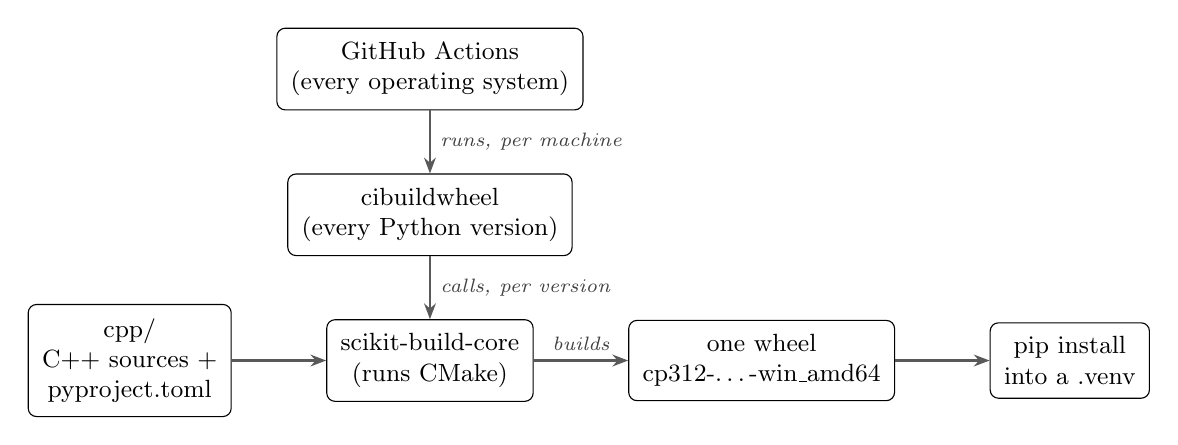
\begin{tikzpicture}[
  box/.style={draw, rounded corners=3pt, align=center, font=\small, inner sep=5pt, fill=white},
  arrow/.style={-{Stealth[length=2mm]}, thick, gray!70!black},
  lbl/.style={font=\scriptsize\itshape, gray!50!black}]
  \node[box] (src) {\code{cpp/}\\C++ sources +\\\code{pyproject.toml}};
  \node[box, right=12mm of src] (skb) {scikit-build-core\\(runs CMake)};
  \node[box, right=12mm of skb] (whl) {one wheel\\\code{cp312-\dots-win\_amd64}};
  \node[box, above=8mm of skb] (cibw) {cibuildwheel\\(every Python version)};
  \node[box, above=8mm of cibw] (gha) {GitHub Actions\\(every operating system)};
  \node[box, right=12mm of whl] (pip) {pip install\\into a \code{.venv}};
  \draw[arrow] (src) -- (skb);
  \draw[arrow] (skb) -- node[lbl, above]{builds} (whl);
  \draw[arrow] (whl) -- (pip);
  \draw[arrow] (cibw) -- node[lbl, right]{calls, per version} (skb);
  \draw[arrow] (gha) -- node[lbl, right]{runs, per machine} (cibw);
\end{tikzpicture}
\end{center}

\begin{center}\small
\begin{tabularx}{\linewidth}{@{}l X@{}}
\toprule
File & Role \\
\midrule
\code{cpp/pyproject.toml} & what the package is and how to build it (scikit-build-core) and how to
  build all variants (cibuildwheel) \\
\code{cpp/bindings/CMakeLists.txt} & the extension modules and what goes into the wheel \\
\code{cpp/scripts/build\_wheels.sh}, \code{.ps1} & all wheels of \emph{this} machine (macOS/Linux,
  Windows) \\
\code{.github/workflows/wheels.yml} & all wheels of \emph{all} machines, in GitHub's cloud \\
\code{nabia\_python/scripts/setup\_env.sh}, \code{.ps1} & installs a wheel into the Python project \\
\bottomrule
\end{tabularx}
\end{center}

%==============================================================================
\section{Wheels}

\subsection{Anatomy of a wheel}

A wheel is a \textbf{zip file} with the extension \code{.whl}. Look inside one:
\begin{lstlisting}[language=bash]
$ python -m zipfile -l dist/nabia_python_bridge-0.1.0-cp314-cp314-macosx_13_0_arm64.whl
nabia_python_bridge/__init__.py
nabia_python_bridge/frames.py                       ... and the other .py files
nabia_python_bridge/_core.cpython-314-darwin.so     the whole C++ library, compiled
nabia_python_bridge/_rb_backtest.cpython-314-darwin.so
nabia_python_bridge-0.1.0.dist-info/METADATA        name, version, dependencies, README
nabia_python_bridge-0.1.0.dist-info/WHEEL           wheel format and tags
nabia_python_bridge-0.1.0.dist-info/RECORD          every file with its SHA-256 hash and size
\end{lstlisting}
\begin{itemize}
  \item The files are laid out \emph{exactly as they will be installed}: installing is unzipping
        into \code{site-packages}. Nothing is compiled at install time.
  \item \code{METADATA} lists the dependencies (\code{Requires-Dist: numpy>=1.24}), which pip
        installs too.
  \item \code{WHEEL} says \code{Root-Is-Purelib: false} (it contains compiled code) and repeats
        the tag.
  \item \code{RECORD} lets pip verify the files and uninstall them later.
\end{itemize}

\subsubsection{The filename is the compatibility contract}
\begin{center}
\code{nabia\_python\_bridge}\,-\,\code{0.1.0}\,-\,\code{cp314}\,-\,\code{cp314}\,-\,\code{macosx\_13\_0\_arm64}\,.whl
\end{center}
\begin{center}\small
\begin{tabularx}{\linewidth}{@{}l l X@{}}
\toprule
Part & Name & Meaning \\
\midrule
\code{nabia\_python\_bridge} & distribution & the package name (\code{project.name}) \\
\code{0.1.0} & version & \code{project.version} \\
\code{cp314} & Python tag & which Python implementation and version can run it: CPython 3.14 \\
\code{cp314} & ABI tag & which binary interface the compiled code uses. \code{abi3} would mean
  the stable ABI (one wheel for many versions); pybind11 modules use the full API, so it is the
  version itself \\
\code{macosx\_13\_0\_arm64} & platform tag & operating system, its minimum version, and the
  architecture \\
\bottomrule
\end{tabularx}
\end{center}

Platform tags you will meet:
\begin{description}
  \item[\code{manylinux\_2\_28\_x86\_64}, \code{\_aarch64}] Linux with glibc 2.28 or newer (Debian
        10+, Ubuntu 20.04+, RHEL 8+). ``Many'' Linux distributions, because the wheel only uses
        libraries every one of them has, in versions at least that old. It is built inside an old
        Linux container on purpose: code compiled against an old glibc runs on newer ones, not the
        reverse.
  \item[\code{macosx\_13\_0\_arm64}, \code{\_x86\_64}] macOS 13 or newer, on Apple silicon or Intel.
        The number comes from \code{MACOSX\_DEPLOYMENT\_TARGET} at build time; it tells the compiler
        which macOS APIs it may use.
  \item[\code{win\_amd64}, \code{win\_arm64}] 64-bit Windows on Intel/AMD, or on ARM.
  \item[\code{any}] no compiled code. The Python project \code{nabia} would
        produce \code{py3-none-any} wheels: one file for every platform.
\end{description}

\subsubsection{How pip chooses}
pip computes the list of tags the running interpreter supports, most specific first, and picks
the first wheel that matches. See the list with \cmd|python -m pip debug --verbose|. If no wheel
matches, pip falls back to the \textbf{sdist} (source distribution, a \code{.tar.gz} of the
sources) and compiles it, which needs CMake and a C++20 compiler on that machine. That is why
binary packages publish one wheel per platform and Python version: users then never compile.

\subsection{Building one wheel}

\subsubsection{The build interface: \texorpdfstring{\code{[build-system]}}{[build-system]}}
pip does not know CMake. Since PEP~517, a project declares a \emph{build backend} that pip calls
in a fresh, isolated environment:
\filepiece{pyproject-build-system}{toml}{\code{cpp/pyproject.toml}: which backend builds the wheel}
\begin{enumerate}
  \item pip (or \code{python -m build}, or \code{uv build}) creates a temporary virtual environment
        and installs \code{requires} into it: scikit-build-core and pybind11.
  \item It calls the backend's \code{build\_wheel()}.
  \item scikit-build-core configures and builds the CMake project, runs the CMake install step into
        a staging folder, and zips that folder into a wheel with its \code{dist-info}.
\end{enumerate}

\subsubsection{What the package is: \texorpdfstring{\code{[project]}}{[project]}}
\filepiece{pyproject-project}{toml}{\code{cpp/pyproject.toml}: package metadata (becomes \code{METADATA})}
\code{dependencies} are installed by pip with the wheel. Optional groups are installed only on
request, for example with \cmd|pip install "nabia_python_bridge[test]"|:
\filepiece{pyproject-project-optional-dependencies}{toml}{\code{cpp/pyproject.toml}: optional dependency groups}

\subsubsection{How CMake is driven: \texorpdfstring{\code{[tool.scikit-build]}}{[tool.scikit-build]}}
\filepiece{pyproject-tool-scikit-build}{toml}{\code{cpp/pyproject.toml}: scikit-build-core settings}
\begin{itemize}
  \item \code{cmake.source-dir} is the folder with the top \code{CMakeLists.txt}: \code{cpp/} itself.
  \item \code{wheel.packages = []}: scikit-build-core copies no Python folder by itself; CMake
        installs everything (below). This keeps development leftovers out of the wheel.
  \item \code{build-dir} keeps a build folder per wheel tag, so rebuilding is incremental.
  \item \code{sdist.exclude} keeps build folders and documentation out of the source package.
\end{itemize}
\filepiece{pyproject-tool-scikit-build-cmake-define}{toml}{\code{cpp/pyproject.toml}: CMake options for wheel builds}
These are ordinary CMake cache variables, as with \code{-D} on the command line: only the bindings
are built (no tests, apps, examples or PDFs), and static libraries are compiled as
position-independent code so they can be linked into a shared module on Linux.

\subsubsection{What goes into the wheel: CMake install rules}
\filepiece{bindings-cmake}{cmake}{\code{cpp/bindings/CMakeLists.txt}: the modules and the install rules}
\code{SKBUILD} is defined only when scikit-build-core runs CMake. Then the two modules and the
\code{.py} files are \code{install}ed to \code{nabia\_python\_bridge/}, which becomes that folder
inside the wheel. They belong to the install \emph{component} \code{python}, and
\code{install.components = ["python"]} in \code{pyproject.toml} installs only that component:
dependencies that CMake downloads have install rules of their own (Eigen installs its 600 headers),
which would otherwise land in every wheel built where Eigen is not installed, as on CI runners. In a normal CMake build (CLion, preset \code{python-bridge}) the modules are
instead written next to the \code{.py} files, for debugging from the source tree.

\begin{note}{Static linking.}
nabia, iir1 and the app's parser are static libraries, and Eigen is header-only, so all of their
code is \emph{inside} \code{\_core}: the wheel needs only the system C++ runtime. A wheel that links
a shared library (say \code{libfoo.so}) must carry a copy; cibuildwheel's \emph{repair} step
(\S\ref{t:sec:cibw}) does that.
\end{note}

\subsubsection{Try it}
\begin{lstlisting}[language=bash]
nabia_python/.venv/bin/python -m pip wheel ./cpp --no-deps -w dist     # one wheel, this Python
MACOSX_DEPLOYMENT_TARGET=13.0 nabia_python/.venv/bin/python -m pip wheel ./cpp --no-deps -w dist
uv build --wheel --python 3.12 --out-dir dist cpp                # with uv, another Python
uv build --sdist --out-dir dist cpp                              # the source package
\end{lstlisting}

\subsection{Installing and using a wheel}

\begin{lstlisting}[language=bash]
python -m venv .venv                                    # an isolated environment
.venv/bin/pip install --no-index --find-links dist nabia_python_bridge
\end{lstlisting}
\begin{itemize}
  \item \code{--find-links dist} adds a folder of wheels as a source; \code{--no-index} turns PyPI
        off, so the package must come from that folder.
  \item pip picks the matching file, reads its dependencies, installs them, unzips the wheel into
        \code{.venv/lib/python3.x/site-packages/}, and keeps its \code{dist-info} there.
  \item \code{import nabia\_python\_bridge} finds the folder; \code{\_\_init\_\_.py} imports
        \code{\_core}, and the operating system's loader maps the \code{.so} into the process.
\end{itemize}

\paragraph{Same version, new build.} pip skips a package whose version is already installed. After
rebuilding the C++ code without changing the version, reinstall explicitly:
\cmd|pip install --force-reinstall --no-deps ...|. The setup scripts do that every time:
\filepiece{setup-env-sh}{bash}{\code{nabia\_python/scripts/setup\_env.sh}: the wheel, then the project in editable mode}

\paragraph{Editable installs.} \cmd|pip install -e nabia_python| does not copy \code{nabia\_python/nabia}: it
installs a pointer to the source folder, so edits are live. That is how \code{nabia\_python} is installed,
while the C++ arrives as a finished wheel.

%==============================================================================
\section{Many wheels}

\subsection{All Python versions on one machine}
On macOS and Linux, \code{build\_wheels.sh} loops over versions with uv, which downloads any
missing Python:
\filepiece{build-wheels-sh}{bash}{\code{cpp/scripts/build\_wheels.sh}}
The pattern is the same for every wheel: \emph{build in isolation, install into a clean
environment, run the tests against the installed copy, keep it only if they pass}. Testing the
installed wheel, from outside the source tree, is the point: it catches a file missing from the
wheel, which tests run on the sources would never see.

\subsection{cibuildwheel}\label{t:sec:cibw}
cibuildwheel automates exactly that loop, for every platform, and adds what portable wheels need.
For each \emph{build identifier} --- \code{cp312-manylinux\_x86\_64}, \code{cp313-macosx\_arm64},
\code{cp314-win\_amd64}, \dots --- it:
\begin{enumerate}
  \item gets that Python (on Linux, inside a \code{manylinux} Docker container; on macOS and
        Windows, official installers it downloads);
  \item builds the wheel through the backend, like \code{pip wheel};
  \item \textbf{repairs} it: on Linux \code{auditwheel} checks it only uses allowed system libraries
        and copies others in, then sets the \code{manylinux} tag; on macOS \code{delocate} does the
        same for \code{.dylib}s; on Windows \code{delvewheel} copies the C++ runtime
        \code{msvcp140.dll}, which Python does not ship, into \code{nabia\_python\_bridge.libs/}
        under a unique name, so the wheel works on a PC without the Visual C++ Redistributable;
  \item installs it in a fresh environment with \code{test-extras} and runs \code{test-command};
  \item moves it to the output folder.
\end{enumerate}

\subsubsection{Configuration}
\filepiece{pyproject-tool-cibuildwheel}{toml}{\code{cpp/pyproject.toml}: which wheels, and how to test them}
\begin{itemize}
  \item \code{build} and \code{skip} are glob patterns over identifiers. Here: CPython 3.10--3.14;
        no musl Linux, no 32-bit.
  \item \code{\{project\}} is the folder cibuildwheel was started in (the repository root, so the
        Python project's tests are reachable); \code{\{package\}} would be \code{cpp/}.
  \item Any setting can be overridden by an environment variable: \code{CIBW\_BUILD},
        \code{CIBW\_ARCHS}, \code{CIBW\_TEST\_SKIP}, \dots{} The workflow and the PowerShell script
        use that.
\end{itemize}
\filepiece{pyproject-tool-cibuildwheel-linux}{toml}{Linux: the container image}
\filepiece{pyproject-tool-cibuildwheel-macos}{toml}{macOS: the oldest supported version}

\subsubsection{Running it yourself}
\begin{lstlisting}[language=bash]
pipx run cibuildwheel==4.3.4 --print-build-identifiers --platform linux cpp   # what would be built
pipx run cibuildwheel==4.3.4 --platform linux cpp       # Linux wheels, needs Docker running
pipx run cibuildwheel==4.3.4 --platform macos cpp       # on a Mac
CIBW_BUILD="cp312-*" pipx run cibuildwheel==4.3.4 --platform linux cpp   # one version only
\end{lstlisting}
On Windows, \code{build\_wheels.ps1} wraps the same call: it checks Visual Studio, Git and Python,
installs cibuildwheel in a private environment and runs it from the repository root.
\filepiece{build-wheels-ps1}{PowerShell}{\code{cpp/scripts/build\_wheels.ps1}}

%==============================================================================
\section{GitHub Actions}

\subsection{Concepts}

GitHub Actions runs commands on machines in GitHub's cloud when something happens in the
repository. The vocabulary:
\begin{description}
  \item[Workflow] a YAML file in \code{.github/workflows/}. GitHub reads every file there. It must be
        at the repository root (not in \code{cpp/}).
  \item[Event] what starts it: a push, a tag, a pull request, a schedule, or a manual start
        (\code{workflow\_dispatch}). A manual start requires the workflow to exist on the default
        branch.
  \item[Run] one execution of a workflow, with a number and a page (Actions tab).
  \item[Job] a unit of work on \emph{one fresh machine}. Jobs run in parallel unless one
        \code{needs} another. Nothing on disk survives from one job to the next.
  \item[Runner] the machine: \code{ubuntu-24.04}, \code{ubuntu-24.04-arm}, \code{macos-14} (Apple
        silicon), \code{windows-latest}, \dots{} A fresh virtual machine each time.
  \item[Step] one command (\code{run:}) or one reusable \textbf{action} (\code{uses:}) inside a job,
        executed in order. If a step fails, the job stops and fails.
  \item[Action] a packaged step published in a repository, used as \code{owner/repo@version}:
        \code{actions/checkout@v5} clones the repository, \code{pypa/cibuildwheel@v4.3.4} runs
        cibuildwheel, \code{actions/upload-artifact@v4} saves files.
  \item[Artifact] files a job uploads to the run, to download later or in another job: the way to
        pass wheels from the build jobs to the collect job, and to you.
  \item[Matrix] one job definition expanded into several jobs, one per combination of values.
\end{description}

\subsubsection{YAML and expressions}
YAML is indentation-based: two spaces per level, \code{key: value}, lists with \code{- }, and
\code{\{ a: 1, b: 2 \}} as a one-line map. Text between \lstinline|${{| and \lstinline|}}| is an
\emph{expression} GitHub evaluates before running anything:
\begin{center}\small
\begin{tabularx}{\linewidth}{@{}l X@{}}
\toprule
Expression & Value \\
\midrule
\code{\$\{\{ matrix.os \}\}} & the current matrix value \\
\code{\$\{\{ github.ref \}\}} & what triggered the run: \code{refs/heads/main}, \code{refs/tags/v0.1.0} \\
\code{\$\{\{ github.token \}\}} & a temporary token for this run, with the job's \code{permissions} \\
\code{\$\{\{ secrets.NAME \}\}} & a secret set in Settings $\to$ Secrets and variables $\to$ Actions \\
\code{\$\{\{ needs.collect.result \}\}} & \code{success}, \code{failure}, \code{cancelled} or \code{skipped} \\
\code{startsWith(a, b)}, \code{!cancelled()} & functions and status checks, used in \code{if:} \\
\bottomrule
\end{tabularx}
\end{center}
Inside \code{run:} scripts, the same information is in environment variables
(\code{\$GITHUB\_REF\_NAME}, \code{\$GITHUB\_REPOSITORY}, \dots).

\subsection{nabia's workflow, piece by piece}

\subsubsection{Name and triggers}
\filepiece{workflow-head}{yaml}{\code{.github/workflows/wheels.yml}: when it runs}
\begin{itemize}
  \item \code{workflow\_dispatch}: the ``Run workflow'' button and \cmd|gh workflow run wheels.yml|.
  \item \code{push: tags: ["v*"]}: pushing a tag such as \code{v0.1.0}. Pushing commits to
        \code{main} does \emph{not} start it (no \code{branches:} filter is given).
  \item \code{pull\_request: paths:}: only pull requests that change those files.
\end{itemize}

\subsubsection{The build matrix}
\filepiece{job-wheels}{yaml}{The \code{wheels} job: one machine per platform}
\begin{itemize}
  \item \code{strategy.matrix.include} lists five combinations, so this definition becomes five
        jobs running in parallel, each with its own \lstinline|${{ matrix.os }}| and
        \lstinline|${{ matrix.archs }}|.
  \item \code{fail-fast: false}: a failure on one platform does not cancel the others.
  \item \code{runs-on} picks the machine from the matrix.
  \item Steps: clone the repository; run cibuildwheel on \code{cpp} (the action installs it and
        passes \code{with:} values as options and \code{env:} values as \code{CIBW\_*} settings);
        upload the wheels as an artifact named after the platform. Each runner builds the five
        Python versions of its platform.
  \item \code{macos-14} is an Apple silicon machine; the \code{x86\_64} entry cross-compiles Intel
        wheels there and tests them under Rosetta.
\end{itemize}

\subsubsection{Collecting everything}
\filepiece{job-collect}{yaml}{The \code{collect} job: every wheel and the sdist in one artifact}
\begin{itemize}
  \item \code{needs: wheels} waits for all five build jobs.
  \item By default a job runs only if everything it needs succeeded. \lstinline|if: ${{ !cancelled() }}|
        overrides that: it runs even if a platform failed, so the good wheels are not lost.
  \item \code{download-artifact} with \code{pattern} and \code{merge-multiple} puts the files of all
        \code{wheels-*} artifacts into one folder.
  \item \code{pipx run build --sdist} builds the source package, the fallback for platforms without
        a wheel.
\end{itemize}

\subsubsection{Publishing a release}
\filepiece{job-release}{yaml}{The \code{release} job: a GitHub Release on version tags}
\begin{itemize}
  \item The \code{if:} makes it run only for tags starting with \code{v}, and only if collecting
        succeeded. On manual runs it shows as \emph{skipped}.
  \item \code{permissions: contents: write}: the run's token is read-only by default; creating a
        release needs write access, granted to this job only.
  \item \code{gh} (the GitHub CLI, installed on every runner) creates the release with all files
        attached and notes generated from the commits since the previous tag.
\end{itemize}

\subsubsection{Testing the Windows scripts}
\filepiece{job-windows-script}{yaml}{The \code{windows-script} job}
\code{actions/setup-python} installs a Python and puts it on the \code{PATH};
\code{shell: pwsh} runs the steps with PowerShell. The job builds one wheel with
\code{build\_wheels.ps1}, installs it with \code{setup\_env.ps1}, and runs the Python project's
tests: the scripts a Windows user would run, run on Windows.

%==============================================================================
\section{Doing it yourself}

\subsection{Writing a job}
A recipe:
\begin{enumerate}
  \item \textbf{Pick the machine} (\code{runs-on}), or several with a matrix.
  \item \textbf{Start with \code{actions/checkout}}: a runner starts empty.
  \item \textbf{Install what is missing}: \code{actions/setup-python} for a given Python; compilers,
        CMake, Git and \code{gh} are preinstalled on GitHub's images.
  \item \textbf{Run commands} with \code{run:}, one step per logical action, each with a
        \code{name:} so the log reads well. Use \code{working-directory:} instead of \code{cd}.
  \item \textbf{Keep results} with \code{upload-artifact}; get them in another job with
        \code{needs:} and \code{download-artifact}.
  \item \textbf{Grant only the permissions needed}, per job.
\end{enumerate}
The examples below are not in the workflow; paste them under \code{jobs:} to use them.

\subsubsection{Example: the C++ tests on Linux and macOS}
\begin{lstlisting}[language=yaml]
  cpp-tests:
    name: C++ tests ${{ matrix.os }}
    strategy:
      fail-fast: false
      matrix:
        os: [ubuntu-24.04, macos-14]
    runs-on: ${{ matrix.os }}
    defaults:
      run:
        working-directory: cpp
    steps:
      - uses: actions/checkout@v5
      - name: Configure
        run: cmake --preset release -DNABIA_BUILD_DOCS=OFF
      - name: Build
        run: cmake --build --preset release -j 4
      - name: Test
        run: ctest --preset release
\end{lstlisting}
A list under \code{matrix} (\code{os: [a, b]}) is the short form of \code{include}; with several
lists, the matrix is their cross product.

\subsubsection{Example: the Python project's tests against the Linux wheel}
\begin{lstlisting}[language=yaml]
  python-tests:
    needs: wheels
    runs-on: ubuntu-24.04
    steps:
      - uses: actions/checkout@v5
      - uses: actions/setup-python@v5
        with:
          python-version: "3.12"
      - uses: actions/download-artifact@v4
        with:
          name: wheels-ubuntu-24.04-x86_64
          path: dist
      - name: Install the wheel and nabia
        run: PYTHON=python nabia_python/scripts/setup_env.sh
      - name: Tests
        working-directory: nabia_python
        run: .venv/bin/python -m pytest -q
\end{lstlisting}

\subsubsection{Example: publishing to PyPI without a password}
PyPI's \emph{trusted publishing} lets a workflow upload without storing a token: on pypi.org, under
the project's Publishing settings, register this repository, the workflow file \code{wheels.yml}
and an environment name (\code{pypi}). Then:
\begin{lstlisting}[language=yaml]
  pypi:
    needs: collect
    if: ${{ startsWith(github.ref, 'refs/tags/v') }}
    runs-on: ubuntu-24.04
    environment: pypi              # optional approval rules live in Settings > Environments
    permissions:
      id-token: write              # proves to PyPI which workflow is uploading
    steps:
      - uses: actions/download-artifact@v4
        with:
          name: all-wheels
          path: dist
      - uses: pypa/gh-action-pypi-publish@release/v1
\end{lstlisting}
Every upload needs a new version number in \code{cpp/pyproject.toml}: PyPI never accepts the same
version twice. Try it first on test.pypi.org (\code{with: repository-url:
https://test.pypi.org/legacy/}).

\subsubsection{Useful extras}
\begin{lstlisting}[language=yaml]
concurrency:                       # top level: a new run of the same branch cancels the older one
  group: wheels-${{ github.ref }}
  cancel-in-progress: true

    timeout-minutes: 60            # in a job: stop a hung job early (default 360)

      - uses: actions/cache@v4     # in steps: reuse downloads between runs
        with:
          path: ~/.cache/pip
          key: pip-${{ runner.os }}-${{ hashFiles('cpp/pyproject.toml') }}
\end{lstlisting}

\subsection{Running, watching and debugging}

\subsubsection{From the terminal}
\begin{center}\small
\begin{tabularx}{\linewidth}{@{}l X@{}}
\toprule
Command & Does \\
\midrule
\code{gh workflow run wheels.yml} & starts a run (the file must be on \code{main}) \\
\code{gh run list --workflow wheels.yml} & recent runs with their ids and status \\
\code{gh run watch \textless{}id\textgreater{}} & live status until it finishes \\
\code{gh run view \textless{}id\textgreater{}} & jobs and their results \\
\code{gh run view \textless{}id\textgreater{} --log-failed} & the log lines of failed steps (after the run ends) \\
\code{gh run rerun \textless{}id\textgreater{} --failed} & reruns only the failed jobs \\
\code{gh run cancel \textless{}id\textgreater{}} & stops a run \\
\code{gh run download \textless{}id\textgreater{} -n all-wheels -D dist} & downloads an artifact \\
\code{gh release list}, \code{gh release view v0.1.0} & releases and their files \\
\bottomrule
\end{tabularx}
\end{center}

\subsubsection{On the web}
Repository $\to$ \textbf{Actions} tab $\to$ \emph{wheels} in the sidebar $\to$ a run. The summary
page shows the jobs as a graph (\code{wheels} $\to$ \code{collect} $\to$ \code{release}) and, at the
bottom, the \textbf{Artifacts}. Click a job, then a step, to read its log; the gear menu downloads
the full log. \emph{Re-run jobs} and \emph{Cancel workflow} are at the top right.

\subsubsection{Reading a failure}
cibuildwheel ends a failed build with a summary such as
\begin{lstlisting}
Error: cibuildwheel: Command [... '-m', 'build', '.../cpp', '--wheel', ...] failed with code 1.
\end{lstlisting}
which only says \emph{that} the build failed. The cause is above it: search the log for
\code{error:} (compiler), \code{CMake Error}, \code{FAILED:} (the file that did not compile) or a
Python traceback. Failures met while setting up this workflow, and their fixes:
\begin{center}\small
\begin{tabularx}{\linewidth}{@{}>{\raggedright\arraybackslash}X >{\raggedright\arraybackslash}X >{\raggedright\arraybackslash}X@{}}
\toprule
Log & Cause & Fix \\
\midrule
\code{HTTP 404: workflow wheels.yml not found on the default branch} & the file was not pushed to
  \code{main} & commit and push it \\
\code{AssertionError: uv not found} (macOS, Windows) & \code{build-frontend = "build[uv]"} needs uv
  on the runner & use the default frontend \\
\code{error: no member named 'jthread' in namespace 'std'} & the Xcode 15 libc++ of \code{macos-14}
  is older than the local one & a joining \code{std::thread} wrapper \\
\code{'from\_chars' is unavailable: introduced in macOS 26.0} & a deployment target older than the
  library function & \code{strtod}/\code{snprintf} \\
\code{The run was canceled by @user} & cancelled by hand & nothing; rerun if needed \\
an \code{include/} folder (Eigen headers) in the CI wheels & install rules of a downloaded dependency &
  install only the component \code{python} \\
\bottomrule
\end{tabularx}
\end{center}
\begin{note}{Reproduce locally first.}
A CI round trip takes minutes; most failures reproduce on your machine:
\cmd|cpp/scripts/build_wheels.sh 3.12| for macOS, \cmd|pipx run cibuildwheel --platform linux cpp|
with Docker for Linux, an older \code{MACOSX\_DEPLOYMENT\_TARGET} for macOS availability errors.
\end{note}

\subsection{Releasing}
\begin{center}\small
\begin{tabularx}{\linewidth}{@{}l >{\raggedright\arraybackslash}X >{\raggedright\arraybackslash}X@{}}
\toprule
Where & Who can install & How \\
\midrule
Run artifacts & you and collaborators, logged in, for 90 days & \code{gh run download} \\
GitHub Release & anyone who can see the repository (it is private: collaborators); permanent &
  \code{git tag v0.1.0 \&\& git push origin v0.1.0}, then download from the Releases page \\
PyPI & anyone: \code{pip install nabia-python-bridge} & trusted publishing job, new version each time \\
\bottomrule
\end{tabularx}
\end{center}
A release checklist:
\begin{enumerate}
  \item Set the version in \code{cpp/pyproject.toml} (and in \code{nabia\_python/} if it is
        published too); commit and push.
  \item Start a manual run and check every job is green.
  \item Tag and push the tag: \cmd|git tag v0.2.0 && git push origin v0.2.0|. The tag run builds
        again and creates the release.
\end{enumerate}

\subsection{Costs and limits}
\begin{itemize}
  \item \textbf{Minutes.} The repository is private, so runs use the account's included Actions
        minutes, and macOS and Windows minutes count more than Linux ones (see Settings $\to$
        Billing). A full run builds 25 wheels on five machines plus the Windows script job; trigger
        it when needed rather than on every push.
  \item \textbf{Storage.} Artifacts count toward the account's storage until they expire (90 days
        by default); releases do not expire.
  \item \textbf{Versions.} Pin actions to versions (\code{@v5}, \code{@v4.3.4}) so a new release of an
        action cannot change the build unannounced; update them deliberately.
\end{itemize}



\part{The Python package}\label{part:python}
% The nabia Python package on the wheel: the library from Python, backtests, market data, analytics.

\chapter{Portfolio backtests: \texorpdfstring{\code{nabia.backtest}}{nabia.backtest}}\label{p:sec:bindings}
\code{nabia.portfolio} runs the C++ portfolio engine through \code{\_rb\_backtest}, a module of
the wheel's package \code{nabia\_python\_bridge}. The module reuses the command-line
application's JSON parser: Python and the command line accept the same parameters with the same
error messages (Chapter~\ref{c:sec:rbbindings}). Data crosses the boundary
in simple forms: dates as \code{int64} days since 1970-01-01, prices as a \code{float64} matrix,
and parameters as JSON text.

Two functions are exposed:
\begin{itemize}
  \item \code{nabia.backtest(prices, params, budget\_schedule=None)} returns a result with
        pandas frames and metrics;
  \item \code{nabia.latest\_weights(prices, params)} solves only the last rebalance: the target weights
        to hold now.
\end{itemize}
\snippet{py_backtest_inputs}{Python}{pandas to C++}
\begin{codepointers}
  \codeitem{py_backtest}{Python \code{backtest}}
  \codeitem{py_latest_weights}{Python \code{latest\_weights}}
  \codeitem{py_to_days}{dates to day numbers}
\end{codepointers}

%==============================================================================


\chapter{Market data}\label{p:sec:marketdata}

\section{Universe and sources}
The default download universe has four asset classes:
\begin{itemize}
  \item equity indices: S\&P 500, Nasdaq 100, Russell 2000, Euro Stoxx 50, DAX, FTSE 100,
        Nikkei 225, Hang Seng;
  \item US Treasury futures: 2Y, 5Y, 10Y, Bond, Ultra Bond;
  \item commodity futures: WTI, Brent, natural gas, gold, silver, copper, corn, wheat,
        soybeans;
  \item crypto against USD: BTC, ETH, SOL, XRP, ADA, LTC.
\end{itemize}
The AI portfolio uses the nine assets of Table~\ref{p:tab:universe-default}.

\begin{table}[ht]\centering\small
\caption{A default nine-asset portfolio universe.}\label{p:tab:universe-default}
\begin{tabular}{@{}lll@{}}
\toprule
Symbol & Asset & Class \\
\midrule
\code{\textasciicircum GSPC} & S\&P 500 & equity index \\
\code{\textasciicircum STOXX50E} & Euro Stoxx 50 & equity index \\
\code{\textasciicircum N225} & Nikkei 225 & equity index \\
\code{ZN=F} & US 10-Year T-Note future & bond future \\
\code{ZB=F} & US Treasury Bond future & bond future \\
\code{BZ=F} & Brent crude oil future & commodity \\
\code{GC=F} & Gold future & commodity \\
\code{HG=F} & Copper future & commodity \\
\code{BTC/USD} & Bitcoin & crypto \\
\bottomrule
\end{tabular}
\end{table}

\paragraph{Sources.}
\begin{itemize}
  \item \textbf{Yahoo Finance} (\code{yfinance}) provides indices and futures, in batches.
        Futures are front-month continuous series, which jump at contract rolls. WTI
        settled negative on 2020-04-20, where simple returns are undefined, so the
        portfolio uses Brent.
  \item \textbf{Crypto exchanges} (\code{ccxt}, Coinbase by default) provide daily
        candles from public data, with no key. History is paged in windows of 300 candles.
        Windows before a coin's listing date are empty and are stepped over. Paging stops
        if the exchange ignores the start date.
\end{itemize}
\snippet{crypto_fetch}{Python}{Crypto daily candles with pagination}

\section{Storage and incremental updates}
Prices are stored per (symbol, date): open, high, low, close, adjusted close and volume.
\begin{itemize}
  \item \textbf{Upserts.} Writes use \code{INSERT ... ON CONFLICT DO UPDATE}, in the SQLite
        or PostgreSQL dialect, so re-downloading is idempotent and picks up revisions.
  \item \textbf{Incremental updates.} A stored symbol is re-fetched from five days before
        its last date, which corrects recent revisions.
  \item \textbf{Batching.} Symbols are grouped by source and start date.
\end{itemize}
\snippet{upsert_rows}{Python}{Portable upsert}
\snippet{update_market_data}{Python}{Incremental download}
\begin{codepointers}
  \codeitem{universe}{universe}
  \codeitem{yahoo_fetch}{Yahoo source}
  \codeitem{load_prices}{loading a price matrix}
\end{codepointers}

\chapter{Analytics on price frames}\label{p:sec:stats}
\code{nabia.analytics} computes descriptive statistics and trend signals on any
pandas frame of prices (dates by assets).

All statistics use daily close prices up to \code{as\_of}, over
\code{stats\_history\_days} (400) calendar days. Volatilities are annualized with
$\sqrt{252}$, standard deviations are sample standard deviations, and returns are simple
returns.
\begin{description}
  \item[Aligned returns] keep the dates where all assets have a price, then take returns.
        They are used for correlations only. Single-asset statistics use each asset's own
        history.
  \item[Correlation] is the Pearson correlation matrix $\rho$ of the last $w$ aligned
        returns (60 by default, at least 3). The \emph{average correlation} is
        \[
          \bar\rho=\frac{1}{n(n-1)}\sum_{i\ne j}\rho_{ij}.
        \]
  \item[Rolling volatility] is
        $\sigma^{(w)}=\mathrm{sd}\big(r_{T-w+1..T}\big)\sqrt{252}$ for
        $w\in\{20,60,120\}$. The \emph{volatility percentile} is computed from the series
        $v_s$ of rolling 20-day standard deviations over the last 252 dates:
        \[
          \pi=\frac{1}{|v|}\sum_s\mathbf 1[v_s\le v_T].
        \]
        So $\pi=1$ means the highest of the year.
  \item[Past returns] $P_T/P_{T-n}-1$ for $n\in\{21,63,126,252\}$ observations
        (1, 3, 6 and 12 months).
  \item[Moving-average distance] $P_T/\overline P_n-1$, where $\overline P_n$ is the mean
        of the last $n\in\{50,200\}$ prices.
  \item[Volatility-scaled 12-1 momentum]
        \[
          m=\frac{P_{T-21}/P_{T-252}-1}{\mathrm{sd}(r_{T-251..T})\sqrt{252}} .
        \]
        It is the 11-month return ending one month ago, which skips the short-term
        reversal, measured in units of the asset's own annual volatility.
  \item[Drawdowns] over the last 253 prices: $D_t=1-P_t/\max_{s\le t}P_s$. The tools
        report the current value and the maximum.
  \item[Market regime] combines five numbers:
        \begin{itemize}
          \item $\bar\rho$ over 60 and over 252 aligned returns;
          \item the median volatility percentile;
          \item the share of assets above their 200-day average;
          \item the share of assets with a positive 12-month return.
        \end{itemize}
\end{description}
\snippet{trend_signals}{Python}{Trend signals}
\snippet{rolling_volatility}{Python}{Volatilities and their percentile}
\snippet{market_regime}{Python}{Market regime}
\begin{codepointers}
  \codeitem{correlation_matrix}{correlation matrix}
  \codeitem{average_correlation}{average correlation}
\end{codepointers}


\part{Sentiment-modulated risk budgeting}\label{part:sentiment}
% Part VII: the sentiment-modulated risk-budgeting pipeline (nabia_python/nabia/sentiment_rb).

\chapter{Overview of the pipeline}\label{ch:rb-overview}

The pipeline implements the specification \code{doc/sentiment\_risk\_budgeting\_spec.md}: each portfolio asset
(equity, commodity, government bond, credit) is mapped to a set of sentiment indicators, inherited down an
indicator tree; an elastic net per asset aggregates them into one sentiment score; the score is normalized to
$[0,1]$ and modulates the asset's risk budget, or, in long-short mode, decides whether the asset is held long or
short; a risk-budgeting optimizer turns budgets into weights; the result is backtested against plain equal risk
contribution (ERC). News sentiment comes from a language model. Every numerical step that the C++ library
implements runs in the \code{nabia\_python\_bridge} wheel:
\begin{center}\small
\begin{tabularx}{\linewidth}{@{}l X l@{}}
\toprule
Step & Method & nabia \\
\midrule
News aggregation, volatility, smoothing & exponentially weighted averages & \code{signal.exponential\_moving\_average} \\
Elastic net per asset & coordinate descent, $(\alpha,\lambda)$ grid, purged walk-forward CV, block bootstrap & \code{RegressionEngine} (\code{frames.regress}) \\
Normalization (option) & $\Phi(S/\hat\sigma_S)$ & \code{stats.normal\_cdf} \\
Weights & risk budgeting (Spinu), risk contributions & \code{risk.RiskBudgeting}, \code{risk.Volatility} \\
Long-only backtest, ERC benchmark & walk-forward engine with a budget schedule & \code{frames.backtest} \\
Metrics & Sharpe, drawdown, turnover, \dots & \code{strategy.compute\_performance} \\
\bottomrule
\end{tabularx}
\end{center}
pandas and numpy do the bookkeeping (alignment, rolling z-scores, ranks, correlations). The long-short backtest
runs on a small simulator that repeats the engine's accounting with a direction per asset
(\S\ref{sec:rb-simulator}).

\paragraph{Data flow.} For one configuration, \code{run} (\coderef{rb_run}) executes:
\begin{enumerate}
  \item synthetic point-in-time market data, indicators and news (Chapter~\ref{ch:rb-synthetic});
  \item the news pipeline: dedup, triage, scoring, daily digest, node features (Chapter~\ref{ch:rb-news});
  \item point-in-time transforms and the candidate features of each asset (Chapter~\ref{ch:rb-features});
  \item the walk-forward elastic net, the score $S$ and its normalization $s$ (Chapter~\ref{ch:rb-model});
  \item budgets or directions, the weights and the backtests (Chapter~\ref{ch:rb-portfolio});
  \item tables, CSV outputs and figures.
\end{enumerate}
\snippet{rb_run}{Python}{The pipeline for one configuration}

\paragraph{Code layout} (\code{nabia\_python/nabia/sentiment\_rb}):
\begin{center}\small
\begin{tabularx}{\linewidth}{@{}l l X@{}}
\toprule
Folder & Files & Area \\
\midrule
--- & \code{config.py}, \code{pipeline.py}, \code{\_\_main\_\_.py} & settings, \code{run()}, command line and sweep \\
\code{data/} & \code{synthetic.py}, \code{real.py}, \code{example\_news.py} & synthetic data; real prices, indicators and news files; example news \\
\code{features/} & \code{tree.py}, \code{transforms.py} & indicator tree; point-in-time transforms, candidate features, target \\
\code{llm/} & \code{schemas.py}, \code{client.py}, \code{news.py}, \code{lexicon.py}, \code{batch.py} & schemas; mock or cached Anthropic client; dedup, scoring, node features; offline reader; Message Batches \\
\code{model/} & \code{elastic\_net.py} & elastic net per asset, walk-forward $S$ and $s$ \\
\code{portfolio/} & \code{budgets.py}, \code{backtest.py} & budgets and directions; backtests, simulator, checks \\
\code{report/} & \code{tables.py}, \code{figures.py} & report tables and CSV; figures \\
\code{prompts/} & \code{triage\_v1.md}, \dots & versioned prompt files (system and user templates) \\
\bottomrule
\end{tabularx}
\end{center}
All settings are in one dictionary, \code{CONFIG} (\coderef{rb_config}); \code{load\_config}
(\coderef{rb_load_config}) deep-merges a JSON file of overrides, so taxonomy, features, horizons, bounds, models
and the normalization method change without code edits.

%==============================================================================
\chapter{Indicator tree, point-in-time features and target}\label{ch:rb-features}

\section{The indicator tree}
The taxonomy is a tree of nodes: \code{L0.GLOBAL} (global risk appetite) at the root; the asset classes
\code{L1.EQ}, \code{L1.CMD}, \code{L1.FI}; buckets \code{L2.*} (US and European equities, energy, precious
metals, 10-year Treasuries, high yield); and one node per underlying \code{L3.*}. Each node has a parent; the
ancestors of $n$ are $\anc(n)=\{n,\text{parent}(n),\dots,\code{L0.GLOBAL}\}$ (\coderef{rb_ancestors}). Asset $i$
sits at an L3 node $n_i$ and belongs to an asset class $c(i)\in\{\mathrm{EQ},\mathrm{CMD},\mathrm{GOVT},\mathrm{CREDIT}\}$.

Every feature $k$ is attached to a node $\nu(k)$ and carries a \emph{sign per asset class} $\sigma_{k,c}\in\{-1,0,1\}$
that orients it: after orientation, higher means more bullish for the asset's price. Risk-off is bullish for
government bonds, so a risk-appetite indicator has $\sigma_{k,\mathrm{GOVT}}=-1$. The candidate features of asset
$i$ are those of all its ancestors that are not switched off for its class:
\[
  \mathcal F_i=\{\,k:\ \nu(k)\in\anc(n_i),\ \sigma_{k,c(i)}\ne0\,\}.
\]
Each feature enters once (the matrix is keyed by feature), which the tests check
(\code{test\_assets\_inherit\_every\_ancestor\_feature\_once}).
\snippet{rb_asset_matrix}{Python}{Candidate features of an asset, oriented}

\section{Point-in-time alignment and transforms}
A value observed for date $t$ (\emph{as of} $t$) becomes usable $\ell_k$ days later (\emph{available at}
$t+\ell_k$): a COT report three days, financial-conditions indices five, LLM features one day after the news is
received. The usable series is therefore $\tilde x_{k,t}=x_{k,t-\ell_k}$, and nothing earlier than its
availability is ever used. The series is then made stationary and standardized:
\[
  u_{k,t}=\begin{cases}\tilde x_{k,t}-\tilde x_{k,t-5}&\text{(transform ``diff'')}\\ \tilde x_{k,t}&\text{(transform ``z'')}\end{cases},
  \qquad
  z_{k,t}=\operatorname{clip}_{[-3,3]}\!\left(\frac{u_{k,t}-m_t^{(W)}(u_k)}{s_t^{(W)}(u_k)}\right),
\]
with the rolling mean $m^{(W)}$ and standard deviation $s^{(W)}$ over $W=756$ trading days (about three years,
at least 252 observations). Rolling, not full-sample, statistics keep every value point in time. The oriented
feature of asset $i$ is $\hat z^{(i)}_{k,t}=\sigma_{k,c(i)}\,z_{k,t}$.
\snippet{rb_transform}{Python}{Point in time, stationary, rolling z-score}

\section{The target}
The elastic net predicts the forward vol-scaled return over $h=21$ days,
\[
  y_{i,t}=\frac{P_{i,t+h}/P_{i,t}-1}{\hat\sigma_{i,t}\sqrt h},\qquad
  \hat\sigma_{i,t}^2=\operatorname{EWMA}_{H=20}\big(r_{i,\cdot}^2\big)_t ,
\]
where the exponentially weighted mean of squared daily returns (half-life 20 days, smoothing factor
$\alpha=1-2^{-1/20}$) comes from \code{signal.exponential\_moving\_average}. Scaling by volatility makes targets
comparable across assets and calm or turbulent periods. $y_{i,t}$ is only known at $t+h$, which the training
windows respect (\S\ref{sec:rb-purge}).
\snippet{rb_target}{Python}{Vol-scaled forward return}
\begin{codepointers}
  \codeitem{rb_build_features}{all features: indicators, node LLM features, digest outputs}
  \codeitem{rb_node_sign}{orientation of the latent factors (synthetic data)}
\end{codepointers}

%==============================================================================
\chapter{The LLM news pipeline}\label{ch:rb-news}

\section{Prompts, schemas and the client}
Three prompts, stored as versioned files in \code{prompts/} (system and user templates, separated by a marker):
\begin{description}
  \item[A, triage] (a small model): is the article relevant, which taxonomy nodes does it concern, with which
        relevance and channel (\emph{direct}: the node's asset is the subject; \emph{spillover}: affected through
        a sector, competitor or macro link). Market recaps are marked irrelevant.
  \item[B, scoring] (a stronger model): for each node, the sentiment in $[-1,1]$ for the asset's price over the
        next 1--20 trading days, a confidence, magnitude, horizon, surprise versus expectations, fact type and a
        short rationale. Government bonds: hawkish policy and upside inflation are negative.
  \item[C, digest] (one call per day, on the day's deduplicated headlines): risk appetite, growth tone, inflation
        tone, geopolitical stress, credit tone, central-bank tone per bank, commodity supply tone per complex.
\end{description}
Each response is validated against a pydantic schema (\coderef{rb_triage_schema}, \coderef{rb_score_schema},
\coderef{rb_digest_schema}): numbers in range, categories from closed lists. A malformed response is retried up to
twice, then logged and skipped. Every call is appended to \code{llm\_audit.jsonl} with the prompt version (file
name and hash of its text), the model, a hash of the request, the article or date it concerns, the attempt, and
the raw response, so each score can be reproduced or re-scored. Templates are filled by \code{fill}
(\coderef{rb_fill}).
\snippet{rb_llm_call}{Python}{One LLM call: fill, call, validate, retry, audit}
With \code{--live}, the call goes to the Anthropic API at temperature 0, with the output forced through a tool whose
input schema is the pydantic schema, and the system prompt cached; the SDK retries rate limits and server errors
with exponential backoff. Offline, \code{mock\_response} (\coderef{rb_mock}) answers from the synthetic truth of
the article, with noise, and returns 1\% of first attempts malformed so the retry path is exercised.
\snippet{rb_llm_anthropic}{Python}{The Anthropic call: structured output through a tool}
\paragraph{Look-ahead.} A model trained after an article's date may ``know'' what followed. The pipeline offers
anonymization (entity names replaced by \emph{Entity k} in every prompt, the mapping to node IDs kept outside the
model), and limits live scoring to recent news (\code{llm.live\_days}); out-of-sample performance after the model's
training cutoff is the real validation.

\section{Deduplication and novelty}
A story is often published several times. Each headline is embedded as a hashed bag of words: tokens are
hashed into $d=256$ buckets, counted and normalized, $v_a\in\mathbb R^{256}$, $\|v_a\|=1$ (\coderef{rb_embed}).
Article $a$ joins the cluster of an earlier article $b$ received within 48 hours if $v_a^\top v_b>0.9$. Its
\emph{novelty} is
\[
  \nu_a=\frac1{1+n_a},
\]
with $n_a$ the number of earlier articles of its cluster in the window: 1 for a new story, $\tfrac12$ for the
first repeat, and so on.
\snippet{rb_dedup}{Python}{Clusters and novelty}

\section{Weights and decay-weighted aggregation}
Each (article, node) score $s_a$ gets the weight
\[
  w_a=\text{relevance}_a\times\text{confidence}_a\times\nu_a\times\omega_{\text{source}(a)},
\]
with source weights $\omega$ (wire 1, newspaper 0.8, blog 0.4). The node's sentiment on day $t$ is the
decay-weighted mean of the scores received up to $t$:
\begin{equation}\label{eq:rb-decay}
  \bar s_{n,t}=\frac{\sum_{a:\,t_a\le t}w_a\,s_a\,e^{-\lambda(t-t_a)}}{\sum_{a:\,t_a\le t}w_a\,e^{-\lambda(t-t_a)}},
  \qquad \lambda=\frac{\ln 2}{H},\quad H=3\text{ days}.
\end{equation}
\snippet{rb_weights}{Python}{Weight of each (article, node) score}
\begin{proposition}\label{prop:rb-ema}
Let $X_t=\sum_{a:\,t_a=t}w_as_a$ and $W_t=\sum_{a:\,t_a=t}w_a$ be the day sums, and $E(x)$ the exponential moving
average with smoothing factor $\alpha=1-e^{-\lambda}$ started from zero,
$E_t=\alpha x_t+(1-\alpha)E_{t-1}$, $E_{-1}=0$. Then $\bar s_{n,t}=E_t(X)/E_t(W)$ whenever $E_t(W)>0$.
\end{proposition}
\begin{proof}
Unrolling the recursion, $E_t(x)=\alpha\sum_{j\le t}(1-\alpha)^{t-j}x_j=\alpha\sum_{j\le t}e^{-\lambda(t-j)}x_j$.
Substituting the day sums, $E_t(X)=\alpha\sum_{a}w_as_ae^{-\lambda(t-t_a)}$ and
$E_t(W)=\alpha\sum_{a}w_ae^{-\lambda(t-t_a)}$; the factor $\alpha$ cancels in the ratio, which is
\eqref{eq:rb-decay}.
\end{proof}
The code therefore computes the aggregation with nabia's EWMA, prepending a zero so that it starts from $E_{-1}=0$:
\snippet{rb_ema0}{Python}{Zero-started EWMA (nabia)}

\section{The five features per node}
For every node $n$ and day $t$:
\begin{center}\small
\begin{tabular}{@{}l l l@{}}
\toprule
Feature & Definition & Orientation \\
\midrule
\code{llm\_level} & $\bar s_{n,t}$, eq.~\eqref{eq:rb-decay} & $+$ \\
\code{llm\_volume} & $\log(1+N_{n,t})$, $N$ the day's relevant articles & $-$ (attention spikes on bad news) \\
\code{llm\_dispersion} & standard deviation of the day's scores & $-$ (disagreement) \\
\code{llm\_mom5} & $\bar s_{n,t}-\bar s_{n,t-5}$ & $+$ \\
\code{llm\_surprise} & $\bar s_{n,t}-\frac1{60}\sum_{j<60}\bar s_{n,t-j}$ & $+$ \\
\bottomrule
\end{tabular}
\end{center}
LLM sentiment is defined with respect to the price of the node's asset, so its sign is $+1$ for the node's subtree,
except at \code{L0.GLOBAL}, where it is risk appetite and takes the risk-on sign of each class. Like every indicator
they are lagged (one day), z-scored and oriented (Chapter~\ref{ch:rb-features}).
\snippet{rb_node_features}{Python}{The five LLM features of every node}

\section{The daily digest}
Prompt C's outputs become features of their node, with a sign per class, e.g. inflation tone negative for equities,
bonds and credit but positive for commodities, a hawkish Fed negative for everything, energy supply tightening
positive for the energy bucket (\code{digest\_features} in \coderef{rb_config}). Null outputs (no relevant news for
a central bank) count as neutral.
\begin{codepointers}
  \codeitem{rb_run_news}{the news pipeline: dedup, triage, scoring, digests}
\end{codepointers}

%==============================================================================
\chapter{Elastic net per asset and the sentiment score}\label{ch:rb-model}

\section{The model}
For each asset $i$ and refit date $T$, the elastic net (Chapter~\ref{ch:en}) is fitted on the oriented
candidates $\hat z^{(i)}_{k,t}$, $k\in\mathcal F_i$:
\[
  \min_{\beta_0,\beta}\ \frac1{2n}\sum_{t\in\mathcal T_T}\big(y_{i,t}-\beta_0-\textstyle\sum_k\beta_k\hat z^{(i)}_{k,t}\big)^2
  +\lambda\Big(\alpha\|\beta\|_1+\tfrac{1-\alpha}2\|\beta\|_2^2\Big),
\]
with standardized features, $\alpha\in\{0.1,0.3,0.5,0.7,0.9\}$ and a $\lambda$ path, chosen by cross-validation.
The fit is nabia's regression engine (\code{frames.regress}) with all candidates in one subset, so the engine tunes
only $(\alpha,\lambda)$.

\section{Purged walk-forward training}\label{sec:rb-purge}
Targets overlap: $y_{i,t}$ spans $t+1,\dots,t+h$. Two precautions keep the future out:
\begin{enumerate}
  \item \textbf{The training rows end $h$ days before the refit date}: $\mathcal T_T=\{t\le T-h\}$, the rows whose
        target is known at $T$ (an assertion checks it). The window is expanding (or rolling, by configuration),
        and starts once enough history exists for the z-scores; a missing z-score counts as neutral (0).
  \item \textbf{Walk-forward cross-validation with a gap}: the engine's folds train on the past and validate on
        the next block, with $h$ rows removed between them (\code{validation\_gap}), the analogue of
        \code{TimeSeriesSplit(gap=h)}.
\end{enumerate}
Refits happen at the end of each quarter (or month); the assets of one refit date are fitted in parallel threads,
since the engine releases Python's GIL.
\snippet{rb_fit_at}{Python}{Training rows of one refit: purged and point in time}

\section{Positivity and stability selection}
The features are pre-oriented, so a negative coefficient would be a nonsensical sign flip; the specification asks
for $\beta\ge0$. nabia's elastic net has no sign constraint, so the pipeline applies it by elimination: fit, drop
the features with $\beta_k<0$, refit, until all coefficients are non-negative. At the same time it applies
\emph{stability selection}: each fit includes a moving-block bootstrap of $B=50$ samples (blocks of $h$ rows, so
overlapping targets stay together), and the selection frequency
\[
  \pi_k=\frac1B\sum_{b=1}^B\one\big[\beta^{(b)}_k\ne0\big]
\]
must exceed $0.6$; features below are dropped and the model refitted. If nothing survives, $\beta=0$: the asset's
score is neutral.
\snippet{rb_fit_asset}{Python}{Elastic net with positivity and stability selection}

\section{The score and its normalization}
With the coefficients of the latest refit, the sentiment score is the prediction minus the intercept,
\[
  S_{i,t}=\sum_{k\in\mathcal F_i}\beta_{ik}\,\hat z^{(i)}_{k,t},
\]
so all-zero coefficients give $S=0$. It is normalized to $[0,1]$ without full-sample statistics, which would look
ahead and be dominated by outliers:
\begin{description}
  \item[Rolling percentile] (default): the share of the last $L=756$ scores (computed with the current
        coefficients) below today's, counting ties as half,
        \[
          s^{\mathrm{ts}}_{i,t}=\frac1L\sum_{u=t-L}^{t-1}\Big(\one[S_{i,u}<S_{i,t}]+\tfrac12\,\one[S_{i,u}=S_{i,t}]\Big).
        \]
        The mid-rank makes a constant score (an asset without features) exactly neutral, $s=\tfrac12$.
  \item[Normal CDF]: $s^{\mathrm{ts}}_{i,t}=\Phi\big(S_{i,t}/\hat\sigma_{S,t}\big)$, with the rolling standard
        deviation $\hat\sigma_S$ (\code{stats.normal\_cdf}).
\end{description}
An optional cross-sectional rank across assets,
$s^{\mathrm{xs}}_{i,t}=(\operatorname{rank}_i S_{\cdot,t}-1)/(N-1)$, is blended,
$s=\alpha_{\mathrm{ts}}s^{\mathrm{ts}}+(1-\alpha_{\mathrm{ts}})s^{\mathrm{xs}}$ ($\alpha_{\mathrm{ts}}=1$ by default),
and the result is smoothed by an EWMA with a 5-day half-life. Every value is checked to lie in $[0,1]$.
\snippet{rb_normalize}{Python}{Score and rolling percentile with the current coefficients}
\snippet{rb_blend}{Python}{Cross-sectional blend and EWMA smoothing}

\section{In-sample and out-of-sample diagnostics}
For every refit, the pipeline records the information coefficient (IC, the correlation of the score with the
realized target) on the training rows and on the next, unseen block. In-sample IC above out-of-sample IC measures
overfitting; the report also gives the IC of $S$ and of $s$ per asset and pooled over the whole out-of-sample
period, and the pooled IC of each LLM feature.
\begin{codepointers}
  \codeitem{rb_walk_forward}{walk-forward refits, scores, normalization, IC records}
  \codeitem{rb_tables}{report tables: comparison, IC, snapshot, selection frequencies}
\end{codepointers}

%==============================================================================
\chapter{From sentiment to positions}\label{ch:rb-portfolio}

\section{Risk budgeting}
Given a covariance $\Sigma$ and budgets $b_i>0$, $\sum_ib_i=1$, the risk-budgeting portfolio
(Chapter~\ref{c:sec:riskbudgeting}) solves
\[
  \min_{w>0}\ R(w)-\sum_ib_i\ln w_i,\qquad R(w)=\sqrt{w^\top\Sigma w},
\]
and is rescaled to sum to one. At the optimum the relative risk contributions equal the budgets:
\[
  \mathrm{RC}_i(w)=\frac{w_i(\Sigma w)_i}{w^\top\Sigma w}=b_i .
\]
(The specification's $\tfrac12w^\top\Sigma w$ gives the same weights up to scale.) The pipeline checks this at
every rebalance with nabia's \code{RiskBudgeting} to $10^{-4}$; observed errors are below $10^{-8}$
(\coderef{rb_check_rc}).

\section{Long-only: modulated budgets}
With base budgets $b^0$ (ERC weights per asset) and normalized sentiment $s_i$,
\[
  b_i=\frac{b_i^0\,\big(m_{\min}+(m_{\max}-m_{\min})\,s_i\big)}{\sum_jb_j^0\,\big(m_{\min}+(m_{\max}-m_{\min})\,s_j\big)},
  \qquad m_{\min}=0.5,\ m_{\max}=1.5,
\]
so neutral sentiment ($s=\tfrac12$) keeps $b^0$ and the multiplier ranges over $[0.5,1.5]$. Budgets stay strictly
positive (the log barrier needs $b>0$). The change per rebalance is capped at $\pm25\%$ relative: the budgets are
clipped to $[b^{\mathrm{prev}}(1-c),\,b^{\mathrm{prev}}(1+c)]$ and renormalized, repeatedly.
\snippet{rb_modulate}{Python}{Budget modulation with a change cap}

\section{Long-short: directions}\label{sec:rb-longshort}
In long-short mode, sentiment decides the side of each position and the budgets stay $b^0$ (optionally scaled by
conviction, $s_i$ for a long and $1-s_i$ for a short). The direction $d_i\in\{+1,-1\}$ follows a neutral band with
hysteresis, so an asset hovering around one threshold does not flip back and forth:
\[
  d_{i,t}=\begin{cases}-1&s_{i,t}<s_{\mathrm{short}}\ (0.35)\\ +1&s_{i,t}>s_{\mathrm{long}}\ (0.5)\\ d_{i,t^-}&\text{otherwise.}\end{cases}
\]
\snippet{rb_directions}{Python}{Directions with hysteresis}
A short position earns $-r_i$. With $D=\operatorname{diag}(d)$, the directed returns are $Dr$, whose covariance is
$\Sigma'=D\Sigma D$: a shorted asset's correlations with the others change sign, so it is sized as the hedge or
diversifier it becomes. The optimizer runs on $\Sigma'$ and returns positive exposures $w'$; the weights are
$w=Dw'$.
\begin{proposition}\label{prop:rb-short}
Let $w'>0$ be the risk-budgeting solution on $\Sigma'=D\Sigma D$ with budgets $b$, and $w=Dw'$. Then the risk
contributions of $w$ on the original covariance equal the budgets: $\mathrm{RC}_i(w;\Sigma)=b_i$. Every position,
long or short, carries its risk budget.
\end{proposition}
\begin{proof}
Since $d_i^2=1$, $w^\top\Sigma w=w'^\top D\Sigma Dw'=w'^\top\Sigma'w'$ and
$w_i(\Sigma w)_i=d_iw'_i(\Sigma Dw')_i=w'_i\,(D\Sigma Dw')_i=w'_i(\Sigma'w')_i$. Hence
$\mathrm{RC}_i(w;\Sigma)=\mathrm{RC}_i(w';\Sigma')=b_i$ by optimality of $w'$.
\end{proof}
\snippet{rb_solve}{Python}{Risk budgeting on $D\Sigma D$ (nabia)}

\section{The long-short simulator}\label{sec:rb-simulator}
nabia's backtest engine has no notion of direction, and directions change between rebalances while the covariance
window spans several of them, so flipping columns of its input would mix signs within one window. The simulator
\code{simulate} repeats the engine's accounting (Chapter~\ref{c:sec:engine}) and applies the current directions to
the whole trailing window at each rebalance:
\begin{itemize}
  \item \textbf{Covariance}, the engine's estimator: weights $\omega_j\propto2^{-a_j/H}$ for a row of age $a_j$
        (half-life $H=60$; equal weights for the sample estimator), normalized, and
        \[
          \hat\Sigma=\frac{\sum_j\omega_j(r_j-\bar r)(r_j-\bar r)^\top}{1-\sum_j\omega_j^2},\qquad\bar r=\sum_j\omega_jr_j ,
        \]
        over $W=252$ rows (\coderef{rb_window_cov}).
  \item \textbf{Rebalances} at rows $W-1+kf$, $f=21$; the budgets and directions in force are the last schedule row
        at or before the date.
  \item \textbf{Drift}: between rebalances each holding grows with its return,
        $w\leftarrow w\circ(1+r_t)/(1+w^\top r_t)$; short weights drift the same way.
  \item \textbf{Costs}: at a rebalance the turnover is $\tau=\|w^\ast-w\|_1$ and the cost $c\,\tau$ ($c=5$ bp); the
        net return is $(1+w^\top r_t)(1-c\tau)-1$.
  \item \textbf{Metrics} from the first trade on, with nabia's \code{compute\_performance}.
\end{itemize}
Run with all-long directions, the simulator reproduces nabia's engine: equity to $6.5\times10^{-10}$, weights to
$6\times10^{-9}$, identical Sharpe ratio. The long-only path asserts this on every run, and a test checks it on
independent data (\coderef{rb_test_simulator}); \coderef{rb_test_short} checks Proposition~\ref{prop:rb-short}.
\snippet{rb_simulate}{Python}{The engine's accounting with directions}
\snippet{rb_backtests}{Python}{Benchmark and overlay: same covariance, rebalancing and costs}

%==============================================================================
\chapter{Real data and live scoring}\label{ch:rb-real}

With \code{--data real} (\code{"data": \{"source": "real"\}}), \code{run} replaces the synthetic generators by three
loaders and leaves everything downstream unchanged.

\section{Prices and indicators}
\code{real\_market} downloads daily closes from Yahoo Finance and series from FRED and caches each as a CSV file in
\code{data.cache\_dir}, so a run is reproducible and works offline once the cache exists. The mapping is in
\code{CONFIG["real"]}: an asset ticker per asset (the energy asset uses Brent, since WTI settled negative on 2020-04-20)
and, per indicator, its source:
\begin{center}\small
\begin{tabular}{@{}l l l@{}}
\toprule
Feature & Source & Series \\
\midrule
\code{VIX}, \code{MOVE}, \code{USD} & Yahoo Finance & \code{\^{}VIX}, \code{\^{}MOVE}, \code{DX-Y.NYB} \\
\code{HY\_OAS}, \code{NFCI}, \code{TERM\_PREMIUM} & FRED & \code{BAMLH0A0HYM2}, \code{NFCI}, \code{THREEFYTP10} \\
\code{CRACK} & derived & $(2\,\text{gasoline}+\text{heating oil})\times42/3-\text{crude}$, in \$/barrel \\
\bottomrule
\end{tabular}
\end{center}
Features without a free source are removed from the run. Returns use the US trading calendar, other markets'
holidays forward-filled (at most three days); each indicator is taken as of its last observation on or before each
date, and the publication lags of \code{CONFIG["features"]} then apply as usual. FRED publishes only about three years
of the high-yield OAS; before that the feature is missing and counts as neutral.
\snippet{rb_real_market}{Python}{Real returns and indicator levels}

\section{News files and the offline reader}
\code{load\_news} reads a JSON file of articles with \code{publish\_ts}, \code{received\_ts} (ISO 8601), \code{source},
\code{headline} and \code{body}: the fields a news feed provides. Until one exists, \code{data/example\_news.json} stands
in: \code{example\_news.py} applies the oracle construction of \S\ref{sec:rb-oracle} to the \emph{real} assets' forward
returns (IC 0.2 by default) and writes articles in the real format, so a real-data run has news with a known skill. It
looks ahead on purpose and must be replaced by real news for any conclusion.

Offline, articles without a synthetic truth are read by \code{lexicon\_response}: the node is the taxonomy node whose
name or alias (\code{CONFIG["aliases"]}) is the longest found in the headline, its parent a spillover; the tone is
$\tanh$ of the summed polarities of finance words; recaps are recognized by their wording; the digest averages the day's
tones per node. On the example vocabulary this recovers the five tone levels in order.
\snippet{rb_lexicon_response}{Python}{The offline reading of real-format articles}

\section{Live scoring, the response cache and Message Batches}
With \code{--live}, the days from \code{llm.live\_days} before the end are scored by the model; \code{0} scores every
day. Each call has a key, the hash of the prompt version, the model and the filled request; a valid response is
appended to \code{llm.cache} (\code{data/llm\_cache.jsonl}) and every later call with the same key, in this run or the
next, is served from it, so each article is paid for once and a run can be repeated exactly. With \code{--batch}, the
uncached requests of a run are first submitted as Message Batches, one per stage, because scoring depends on triage and
the digests on the day's articles: all triage requests, then the scoring requests of the relevant articles, then the
digests. Each batch is polled until it ends, its valid responses are cached, and the pipeline's calls that follow are
cache hits; failed entries are retried one by one by the normal path.
\snippet{rb_batch_submit}{Python}{Message Batches: submit, wait, cache}
\begin{codepointers}
  \codeitem{rb_load_news}{news files}
  \codeitem{rb_make_example_news}{example news from real returns}
  \codeitem{rb_llm_request}{cache key of a call}
  \codeitem{rb_llm_prefill}{batch backfill of one stage}
\end{codepointers}

\section{Downloading news: nabia.news}\label{sec:rb-news-download}
The package \code{nabia.news} collects real articles into the JSON format above (\code{python -m nabia.news fetch}):
\begin{description}
  \item[RSS / Atom feeds] (\coderef{rb_news_feeds}): financial media and central banks, parsed with the standard library
        (RFC 822 or ISO 8601 dates, HTML stripped). Feeds carry only recent items, so \code{received\_ts} is the download
        time and history is built by running the download daily.
  \item[GDELT raw files] (\coderef{rb_news_gkg}): GDELT publishes every 15 minutes a file of the English web articles it
        processed, with their page titles. For history, two slices per business day (14:30 and 20:30 UTC) are read in
        memory; titles about the portfolio's topics are kept, established financial outlets first, at most
        \code{--per-day} per day; \code{received\_ts} is the slice's timestamp, when GDELT had the article, so the
        history stays point in time. GDELT's search API (\code{--gdelt}) is also supported but rate-limits hard.
  \item[The store] (\coderef{rb_news_store}): \code{data/news.json}, deduplicated by URL and by normalized headline on the
        same day, appended in place and written atomically; each record keeps its feed and URL.
\end{description}

\section{Scoring with a local model and scores files}
Besides the Anthropic API, the LLM steps can run on a local model served by Ollama (\code{"provider": "ollama"};
\coderef{rb_llm_ollama}): the same prompts, the output constrained to the pydantic schema through Ollama's structured
output, temperature 0, and the same response cache. On the development machine (Apple silicon, 34 GB),
\code{gemma4:26b}, a mixture-of-experts model, was the fastest model with sensible answers: about 85 generated tokens
per second and about 2 s per call, against 12--22 s for a dense 27B model. Serving several requests at once
(\code{OLLAMA\_NUM\_PARALLEL} $>1$) slowed every request several times on that machine (prompts re-read, generation
at a few tokens per second per slot), so a local model is used with one worker.

\code{python -m nabia.news score} runs triage, scoring and the daily digests over a news store and writes a
\emph{scores file} (\coderef{rb_write_scores}): per article its triage and node scores (sentiment, confidence,
relevance, novelty and the resulting weight), per day its digest, with the provider, model and prompt versions. With
\code{--scores} (\code{data.scores\_file}), the pipeline reads it (\coderef{rb_load_scores}), maps every article and
digest to the first trading date at or after its day, and calls no model.

%==============================================================================
\chapter{Synthetic data, experiments and results}\label{ch:rb-synthetic}

\section{Synthetic market data}
So that the pipeline runs offline and its behaviour can be tested against a known truth, the data are synthetic
(\coderef{rb_synthetic_market}). Every taxonomy node $n$ has a latent factor, a standardized AR(1),
$f_{n,t}=\phi f_{n,t-1}+\sqrt{1-\phi^2}\,\varepsilon_{n,t}$, $\phi=0.97$ (half-life about three weeks). Asset $i$'s
daily return is
\[
  r_{i,t}=\frac{\sigma_i}{\sqrt{252}}\Big(\kappa\,\frac{\sum_{n\in\anc(n_i)}\sigma^{\mathrm{f}}_{n,c(i)}f_{n,t}}{\sqrt{|\anc(n_i)|}}
  +\ell_{c(i)}\,g_t+\sqrt{1-\ell_{c(i)}^2}\,\eta_{i,t}\Big)+\mathrm{SR}_{c(i)}\frac{\sigma_i}{252},
\]
with annual volatilities $\sigma_i$, signal strength $\kappa=0.15$, a common shock $g$ with class loadings $\ell$
(government bonds negative), and a risk premium of Sharpe ratio $\mathrm{SR}$ per class; the factor sign
$\sigma^{\mathrm f}$ is the risk-on sign at \code{L0.GLOBAL} and $+1$ below. Each indicator is a noisy reading of
its node's factor with a slowly drifting level (or, for transform ``diff'', a stock whose changes carry the signal);
some indicators are pure noise, for the model to discard.

\section{Synthetic news with a known skill}\label{sec:rb-oracle}
The default news generator is an \emph{oracle} with a set skill (\coderef{rb_news_truth}). For node $n$, let
$x_{n,t}$ be the mean over its assets of the oriented forward target, shifted by the LLM lag so that it starts when
the news becomes usable, and $z_{n,t}$ its standardized value. The node's true tone is
\[
  T_{n,t}=\rho\,z_{n,t}+\sqrt{1-\rho^2}\,\epsilon_{n,t},\qquad\operatorname{corr}(T_{n,t},z_{n,t})=\rho ,
\]
where $\rho$ is the \emph{news IC} (\code{synthetic.sentiment\_ic}, 0.2 by default): 0 is pure noise, 1 perfect
foresight. About four articles a day are drawn (more often for global and asset-class nodes), each with tone
$\tanh(T_{n,t}+0.3\,\epsilon_a)$; 12\% are market recaps (irrelevant) and 10\% re-publications (duplicates); the mock
LLM adds scoring noise; the digest derives from the same truths. The rest of the pipeline is unchanged: it must find
the edge through point-in-time features, the purged elastic net, normalization and the budget rules. Setting
\code{"sentiment": "latent"} ties the news to the latent factors instead.
\snippet{rb_news_truth}{Python}{Oracle news truth}

\paragraph{The information coefficient.} The IC of a signal is its correlation with the subsequent realized return,
here $\operatorname{corr}(S_{i,t},y_{i,t})$, per asset or pooled over assets. Real signals have ICs of a few percent;
by the fundamental law of active management the information ratio grows roughly like
$\mathrm{IC}\times\sqrt{\text{breadth}}$, so small ICs applied often can matter.

\section{Results}
The figures and tables below come from runs with the default configuration (seed 7); \code{doc/build.sh --figures}
regenerates them. Signals start in 2018 after the warm-up of the z-scores and the first training window.

\pipelinefigure{lo_portfolio.png}{Long-only overlay against plain ERC (news IC 0.2): cumulative PnL net of costs,
rolling one-year Sharpe ratio, drawdown, return by year. Shaded: the covariance warm-up before the first
out-of-sample signal.}{fig:rb-lo-portfolio}
\pipelinefigure{lo_budgets.png}{Long-only: modulated budgets against $b^0$, normalized sentiment, weights and
cumulative risk contributions (which track the budgets).}{fig:rb-lo-budgets}
\pipelinefigure{lo_model.png}{Elastic net diagnostics: in-sample against out-of-sample IC per asset and per refit,
and the share of refits in which each feature has a non-zero coefficient.}{fig:rb-lo-model}

\IfFileExists{figures/comparison_long_only.tex}{\begin{table}[htbp]\centering\small
\caption{Long-only overlay against plain ERC (news IC 0.2).}\label{tab:rb-lo}\begin{tabular}{@{}lrr@{}}
\toprule
metric & ERC ($b^0$) & sentiment overlay \\
\midrule
annualized return & -0.0178 & -0.0123 \\
annualized volatility & 0.0503 & 0.0506 \\
sharpe ratio & -0.3313 & -0.2181 \\
max drawdown & 0.2688 & 0.2455 \\
annualized turnover & 0.6737 & 1.0579 \\
total costs & 0.0024 & 0.0038 \\
\bottomrule
\end{tabular}

\end{table}}{}
\IfFileExists{figures/comparison_long_short.tex}{\begin{table}[htbp]\centering\small
\caption{Long-short overlay against plain ERC (news IC 0.2).}\label{tab:rb-ls}\begin{tabular}{@{}lrr@{}}
\toprule
metric & ERC ($b^0$) & sentiment overlay \\
\midrule
annualized return & 0.0448 & 0.0803 \\
annualized volatility & 0.0488 & 0.0445 \\
sharpe ratio & 0.9231 & 1.7574 \\
max drawdown & 0.1236 & 0.0876 \\
annualized turnover & 0.6505 & 5.3629 \\
total costs & 0.0023 & 0.0194 \\
\bottomrule
\end{tabular}

\end{table}}{}

\paragraph{Does correct sentiment produce alpha?} The sweep reruns the pipeline on the same market data for several
news ICs. Overlay Sharpe ratio and excess return over ERC grow with the news IC; below an IC of about 0.1 the
elastic net mostly cannot separate the news from noise, and the market indicators alone give a small edge.
\IfFileExists{figures/sweep_long_only.tex}{\begin{table}[htbp]\centering\small
\caption{News-quality sweep, long-only (ERC Sharpe ratio for reference).}\label{tab:rb-sweep-lo}
\begin{tabular}{@{}lrrrrr@{}}
\toprule
news IC & ERC Sharpe & overlay Sharpe & excess return & IC of $S$ & IC of LLM level \\
\midrule
0.0 & -0.33 & -0.30 & +0.14\% & 0.12 & -0.00 \\
0.05 & -0.33 & -0.30 & +0.14\% & 0.13 & 0.04 \\
0.1 & -0.33 & -0.29 & +0.19\% & 0.16 & 0.08 \\
0.2 & -0.33 & -0.22 & +0.55\% & 0.29 & 0.15 \\
0.3 & -0.33 & -0.14 & +0.94\% & 0.43 & 0.23 \\
0.5 & -0.33 & -0.04 & +1.45\% & 0.62 & 0.37 \\
\bottomrule
\end{tabular}
\end{table}}{}
\IfFileExists{figures/sweep_long_short.tex}{\begin{table}[htbp]\centering\small
\caption{News-quality sweep, long-short.}\label{tab:rb-sweep-ls}
\begin{tabular}{@{}lrrrrr@{}}
\toprule
news IC & ERC Sharpe & overlay Sharpe & excess return & IC of $S$ & IC of LLM level \\
\midrule
0.0 & -0.33 & 0.04 & +1.87\% & 0.12 & -0.00 \\
0.05 & -0.33 & 0.13 & +2.26\% & 0.13 & 0.04 \\
0.1 & -0.33 & 0.60 & +4.73\% & 0.16 & 0.08 \\
0.2 & -0.33 & 1.57 & +9.58\% & 0.29 & 0.15 \\
0.3 & -0.33 & 2.69 & +16.23\% & 0.43 & 0.23 \\
0.5 & -0.33 & 2.91 & +18.08\% & 0.62 & 0.37 \\
\bottomrule
\end{tabular}
\end{table}}{}
\pipelinefigure{sweep_long_only.png}{Long-only sweep: Sharpe ratio, excess return and realized IC against the
news IC.}{fig:rb-sweep-lo}
\pipelinefigure{sweep_long_short.png}{Long-short sweep.}{fig:rb-sweep-ls}
\pipelinefigure{ls_budgets.png}{Long-short: budgets stay $b^0$; the sentiment panel shades the neutral band;
negative weights are short positions.}{fig:rb-ls-budgets}

\paragraph{Reading the results.} Long-only modulation can at most halve or increase by half a budget, capped at
25\% per rebalance, so even good news moves the allocation modestly. Long-short acts on the direction of the view
and captures much more of it, at the price of turnover (several times a year) and costs; with uninformative news it
earns almost nothing, which also shows that no future information leaks through the pipeline. The ERC benchmark's
negative return is a property of this seed's synthetic premiums; only the difference matters.

\section{Running and extending}
Chapter~\ref{ch:guide} lists the commands. The command line (\coderef{rb_main}) runs one configuration or a sweep;
figures are produced by \coderef{rb_plots} and \coderef{rb_plot_sweep}. To use real data, replace
\code{synthetic\_market} and \code{synthetic\_news} (\coderef{rb_synthetic_news}) by loaders returning the same
frames: returns by asset, indicator levels by \emph{as-of} date, and articles with publish and received
timestamps; everything downstream is unchanged.


\part{Verification and limitations}\label{part:verification}
% Part VIII: how each part is tested, and what is known to be limited.

\chapter{Verification}\label{c:sec:verification}
\begin{description}
  \item[C++ (Catch2)] 104 test cases, plus an end-to-end run of the command-line application on its example
        (\code{ctest --preset debug}).
        \begin{itemize}
          \item Results against closed forms: inverse volatility for uncorrelated equal budgets, Gaussian VaR and
                ES, SES and Kalman steady states, filter gains at the band edges.
          \item Optimizer results against known optima, with constraints.
          \item Accounting identities of the portfolio engine to $10^{-15}$.
          \item The elastic net against OLS, the ridge closed form and its optimality conditions; the regression
                engine recovering known factors (exhaustive, forward, in-sample BIC), and bootstrap intervals
                covering the true coefficients.
          \item No look-ahead, thread-count independence, invalid input; the application's JSON and CSV parsing
                and writing.
        \end{itemize}
        The suites run in debug, under AddressSanitizer with UndefinedBehaviorSanitizer, and the multithreaded code
        under ThreadSanitizer.
  \item[Bindings (pytest, \code{nabia\_python/tests/bridge})] every module of \code{nabia\_python\_bridge} against
        closed forms and numpy, and the binding semantics (keyword parameters, Python objectives called from C++
        threads, exceptions, kernel composition, frame alignment, budget schedules). The wheel scripts and
        cibuildwheel run them on every wheel they build, on every platform.
  \item[Python package (\code{nabia\_python/tests})] \code{nabia.backtest} against the command-line application on
        its own example (a copy in \code{tests/data}), schedules and errors; the market data store, sources and
        incremental download against fakes; two opt-in tests (\code{NABIA\_NETWORK\_TESTS=1}) download live data.
  \item[Sentiment pipeline] \code{tests/test\_sentiment\_rb.py}: budgets positive, normalized, neutral at
        $s=\tfrac12$ and within the change cap; directions with hysteresis; shorted positions keeping their risk
        budget (Proposition~\ref{prop:rb-short}); the simulator reproducing nabia's engine; every ancestor feature
        inherited exactly once. Each run also asserts: training rows purged by $h$, normalized scores in $[0,1]$,
        risk contributions equal to the budgets at every rebalance ($<10^{-4}$, observed $<10^{-8}$), and, in
        long-only mode, the simulator matching the engine.
  \item[This document] Its excerpts, code locations and file pieces are extracted at build time; a function that no
        longer exists stops the build.
\end{description}

\chapter{Limitations and future work}\label{c:sec:limitations}
\begin{itemize}
  \item \textbf{Gaussian risk.} VaR and ES are Gaussian; fat tails are not modelled. A historical or Cornish--Fisher
        measure would fit the same interface.
  \item \textbf{Factor regression} has constant coefficients, and its bootstrap is conditional on the selected model
        (Chapter~\ref{c:sec:regression}). Exhaustive search grows as $\binom Nk$.
  \item \textbf{SQP} solves its QP subproblems with the augmented Lagrangian to \code{qp\_tolerance}; on some strongly
        convex mean-variance problems it was seen to stall at its iteration limit, so prefer the augmented Lagrangian
        there until the QP step is made exact (an active-set QP).
  \item \textbf{Wheels} for Linux, Intel macOS and Windows are built and tested in CI only; locally on macOS arm64.
  \item \textbf{Sentiment pipeline.}
        \begin{itemize}
          \item The data and news are synthetic; the results measure how much of a \emph{known} news edge survives
                the pipeline, not the value of real news. Real loaders replace two functions
                (Chapter~\ref{ch:rb-synthetic}).
          \item Positivity is imposed by eliminating negative coefficients and refitting, not by a constrained
                solver; the selected set can differ from a non-negative elastic net's.
          \item LLM scores are uncalibrated model judgements, and backtests before a model's training cutoff are
                optimistic. The live path (\code{--live}) is implemented but scores only the most recent days;
                Message Batches backfills are not implemented.
          \item Long-short turnover is high (several times a year at news IC 0.2); a wider neutral band or higher
                costs show how much of the edge survives trading.
          \item Market data caveats: continuous futures jump at rolls; asynchronous closes bias same-day correlations
                downwards.
        \end{itemize}
\end{itemize}


\appendix

\chapter{Glossary}
\begin{description}\small
  \item[ABI] application binary interface: how compiled code calls other compiled code. CPython's
        changes between minor versions.
  \item[auditwheel, delocate, delvewheel] tools that copy shared libraries into a wheel and fix its
        tag (Linux, macOS, Windows).
  \item[install component] a label on CMake install rules, to install a subset of them.
  \item[build backend / frontend] the backend (scikit-build-core) turns a project into a wheel; the
        frontend (pip, \code{build}, \code{uv build}) calls it in an isolated environment.
  \item[deployment target] the oldest macOS a binary supports.
  \item[editable install] an install that points to the source folder instead of copying it.
  \item[glibc] the GNU C library of Linux; \code{manylinux\_2\_28} means version 2.28 or newer.
  \item[sdist] source distribution: the sources and \code{pyproject.toml}, compiled on install.
  \item[site-packages] the folder of an environment where packages are installed.
  \item[wheel tag] the \code{python-abi-platform} part of a wheel's name.
\end{description}

\begin{thebibliography}{99}
\bibitem{bertsekas1982} D.~P. Bertsekas, \emph{Constrained Optimization and Lagrange Multiplier Methods},
Academic Press, 1982.
\bibitem{birgin2014} E.~G. Birgin and J.~M. Mart\'inez, \emph{Practical Augmented Lagrangian Methods
for Constrained Optimization}, SIAM, 2014.
\bibitem{brown1959} R.~G. Brown, \emph{Statistical Forecasting for Inventory Control}, McGraw-Hill, 1959.
\bibitem{bucy1968} R.~S. Bucy and P.~D. Joseph, \emph{Filtering for Stochastic Processes with Applications to Guidance},
  Interscience, 1968.
\bibitem{durbin2012} J. Durbin and S.~J. Koopman, \emph{Time Series Analysis by State Space Methods}, 2nd ed.,
  Oxford University Press, 2012.
\bibitem{gardner1985} E.~S. Gardner, Exponential smoothing: the state of the art,
  \emph{J. Forecasting} 4 (1985) 1--28.
\bibitem{hager2005} W.~W. Hager and H. Zhang, A new conjugate gradient method with guaranteed
descent and an efficient line search, \emph{SIAM J. Optim.} 16 (2005) 170--192.
\bibitem{han1977} S.-P. Han, A globally convergent method for nonlinear programming,
\emph{J. Optim. Theory Appl.} 22 (1977) 297--309.
\bibitem{hartikainen2010} J. Hartikainen and S. S\"arkk\"a, Kalman filtering and smoothing solutions to temporal
  Gaussian process regression models, \emph{IEEE MLSP} (2010) 379--384.
\bibitem{harvey1989} A.~C. Harvey, \emph{Forecasting, Structural Time Series Models and the Kalman Filter},
  Cambridge University Press, 1989.
\bibitem{hestenes1969} M.~R. Hestenes, Multiplier and gradient methods,
\emph{J. Optim. Theory Appl.} 4 (1969) 303--320.
\bibitem{horn2013} R.~A. Horn and C.~R. Johnson, \emph{Matrix Analysis}, 2nd ed., Cambridge University Press, 2013.
\bibitem{hyndman2008} R.~J. Hyndman, A.~B. Koehler, J.~K. Ord and R.~D. Snyder,
  \emph{Forecasting with Exponential Smoothing: The State Space Approach}, Springer, 2008.
\bibitem{kalman1960} R.~E. Kalman, A new approach to linear filtering and prediction problems,
  \emph{J. Basic Engineering} 82 (1960) 35--45.
\bibitem{liu1989} D.~C. Liu and J.~Nocedal, On the limited memory BFGS method for large scale
optimization, \emph{Math. Programming} 45 (1989) 503--528.
\bibitem{mackay1998} D.~J.~C. MacKay, Introduction to Gaussian processes, in C.~M. Bishop (ed.),
  \emph{Neural Networks and Machine Learning}, Springer, 1998, 133--165.
\bibitem{muth1960} J.~F. Muth, Optimal properties of exponentially weighted forecasts,
  \emph{J. Amer. Statist. Assoc.} 55 (1960) 299--306.
\bibitem{nocedal1980} J.~Nocedal, Updating quasi-Newton matrices with limited storage,
\emph{Math. Comp.} 35 (1980) 773--782.
\bibitem{nocedal2006} J.~Nocedal and S.~J. Wright, \emph{Numerical Optimization}, 2nd ed., Springer,
2006, Chapters 7 and 17.
\bibitem{powell1969} M.~J.~D. Powell, A method for nonlinear constraints in minimization problems,
in R.~Fletcher (ed.), \emph{Optimization}, Academic Press, 1969, 283--298.
\bibitem{powell1978} M.~J.~D. Powell, A fast algorithm for nonlinearly constrained optimization
calculations, in G.~A. Watson (ed.), \emph{Numerical Analysis}, Lecture Notes in
Mathematics 630, Springer, 1978, 144--157.
\bibitem{rasmussen2006} C.~E. Rasmussen and C.~K.~I. Williams, \emph{Gaussian Processes for Machine Learning},
  MIT Press, 2006.
\bibitem{roberts2013} S. Roberts, M. Osborne, M. Ebden, S. Reece, N. Gibson and S. Aigrain,
  Gaussian processes for time-series modelling, \emph{Phil. Trans. R. Soc. A} 371 (2013) 20110550.
\bibitem{rockafellar1973} R.~T. Rockafellar, A dual approach to solving nonlinear programming problems by
unconstrained optimization, \emph{Math. Programming} 5 (1973) 354--373.
\bibitem{rockafellar1976} R.~T. Rockafellar, Augmented Lagrangians and applications of the proximal point
algorithm in convex programming, \emph{Math. Oper. Res.} 1 (1976) 97--116.
\bibitem{rts1965} H.~E. Rauch, F. Tung and C.~T. Striebel, Maximum likelihood estimates of linear dynamic systems,
  \emph{AIAA Journal} 3 (1965) 1445--1450.
\end{thebibliography}


\end{document}
